\chapter{Stellar Component}
	\label{cha:stellar}


The rest of this chapter is structured as follows: firstly we present the kinematic maps for the stellar component of the galaxy (section \ref{sec:stellarKin}) and a look at how they fit on the $\lambda_{R_e}$--ellipticity plane, then, in section \ref{sec:pop} we investigate the stellar populations using the absorption line strength. We conclude by looking at the odd-one-out of the sample NGC 612 in section \ref{sec:NGC612}. We aim to demonstrate that our radio selected sample is no different in the V-band to normal, optically selected ETGs. We achieve this by showing that they are consistent with defining characteristics of ETGs that are accessible able to V-band IFS data. The list of characteristics we investigate in this chapter are (the relevant section is shown in parenthesis):
\begin{itemize}
	\item Dispersion dominated stellar kinematics (section \ref{subsec:maps})
	\item The fast/slow rotator fraction (\ref{subsec:FSfrac})
	\item Absorption line strengths (\ref{subsec:absorption})
	\item Absorption line gradients (\ref{subsec:absorptionGrad})
	\item Mg -- \textsigma relation (\ref{subsec:Mgsigma})
	\item Old and metal rich stellar populations (\ref{subsec:ssp})
	\item KDC age -- size relation (\ref{subsec:popKDC})
\end{itemize}

\section{Kinematics}
	\label{sec:stellarKin}

	\subsection{Maps}
		\label{subsec:maps}

		% \begin{figure*}
      \centering
      \includegraphics[width=0.245\textwidth]{Vmaps/ngc0612_stellar_sigma.png}
      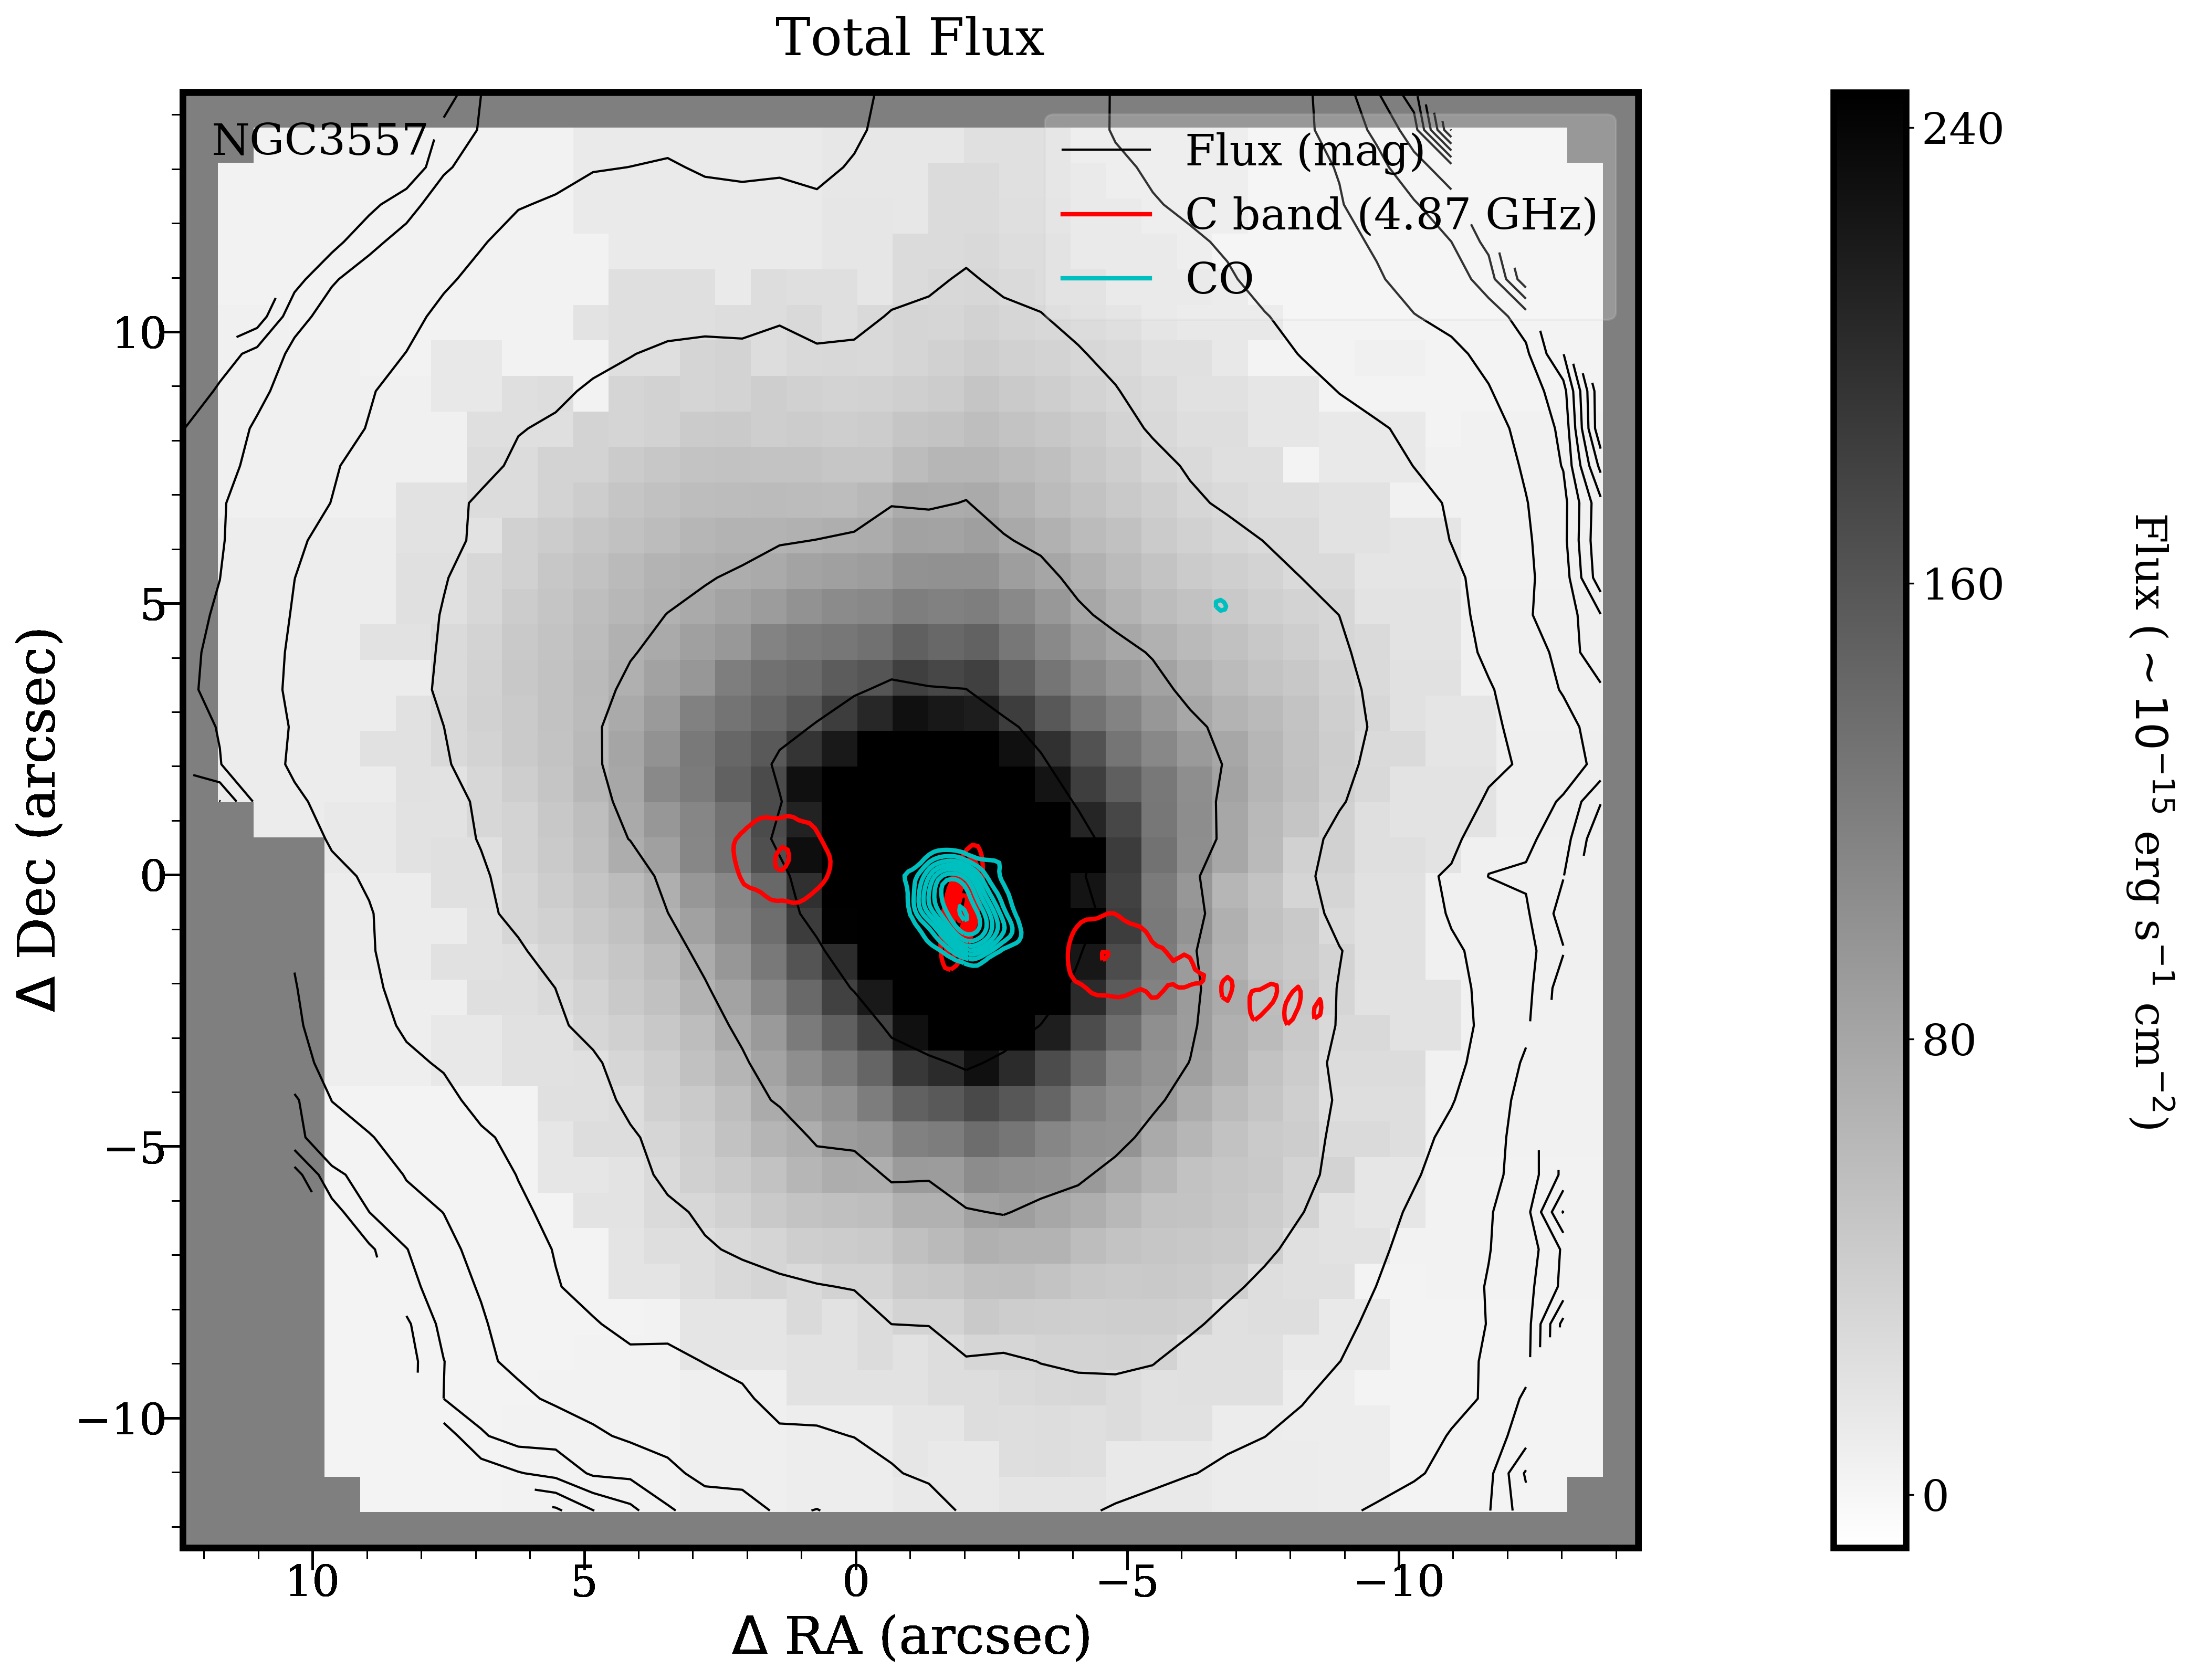
\includegraphics[width=0.245\textwidth]{Vmaps/ngc3557_stellar_img.png}
      \includegraphics[width=0.245\textwidth]{Vmaps/ngc3100_stellar_img.png}
      \includegraphics[width=0.245\textwidth]{Vmaps/ic1459_stellar_img.png}
      \includegraphics[width=0.245\textwidth]{Vmaps/pks0718-34_stellar_img.png}
      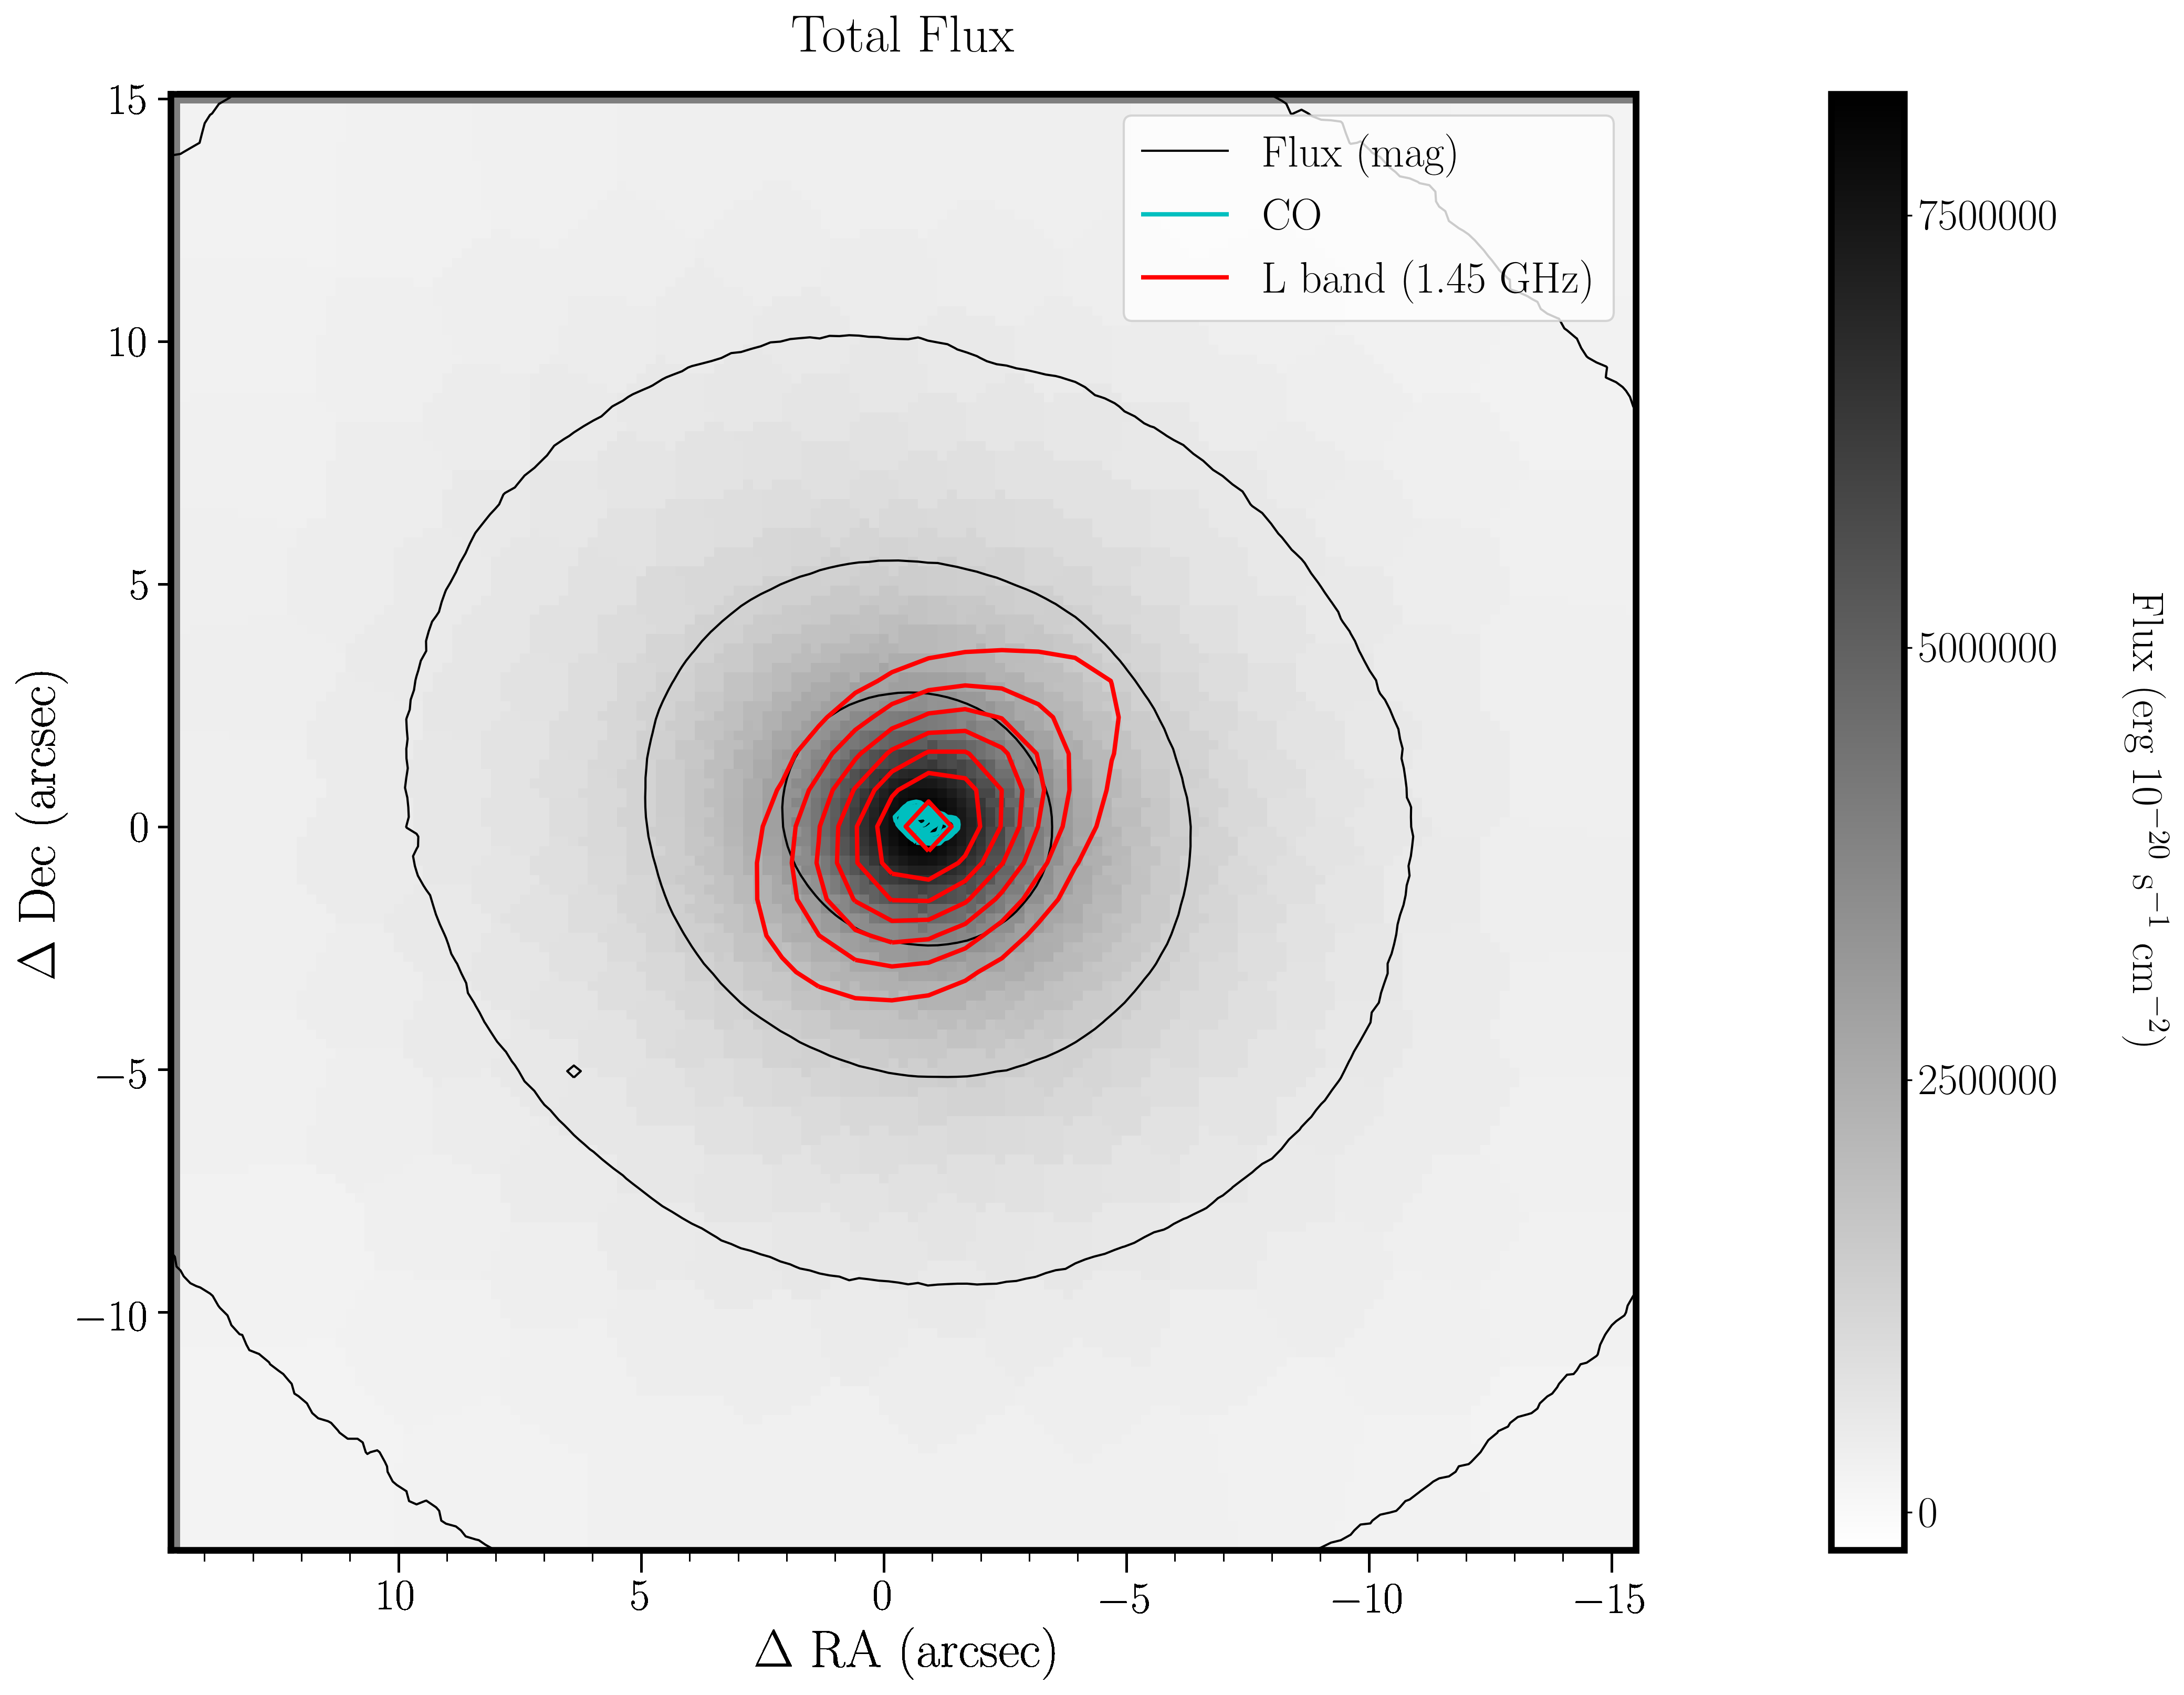
\includegraphics[width=0.245\textwidth]{Vmaps/ic4296_stellar_img.png}
      \includegraphics[width=0.245\textwidth]{Vmaps/ngc7075_stellar_img.png}
      \includegraphics[width=0.245\textwidth]{Vmaps/ic1531_stellar_img.png}
      \includegraphics[width=0.245\textwidth]{Vmaps/ngc1399_stellar_img.png}
      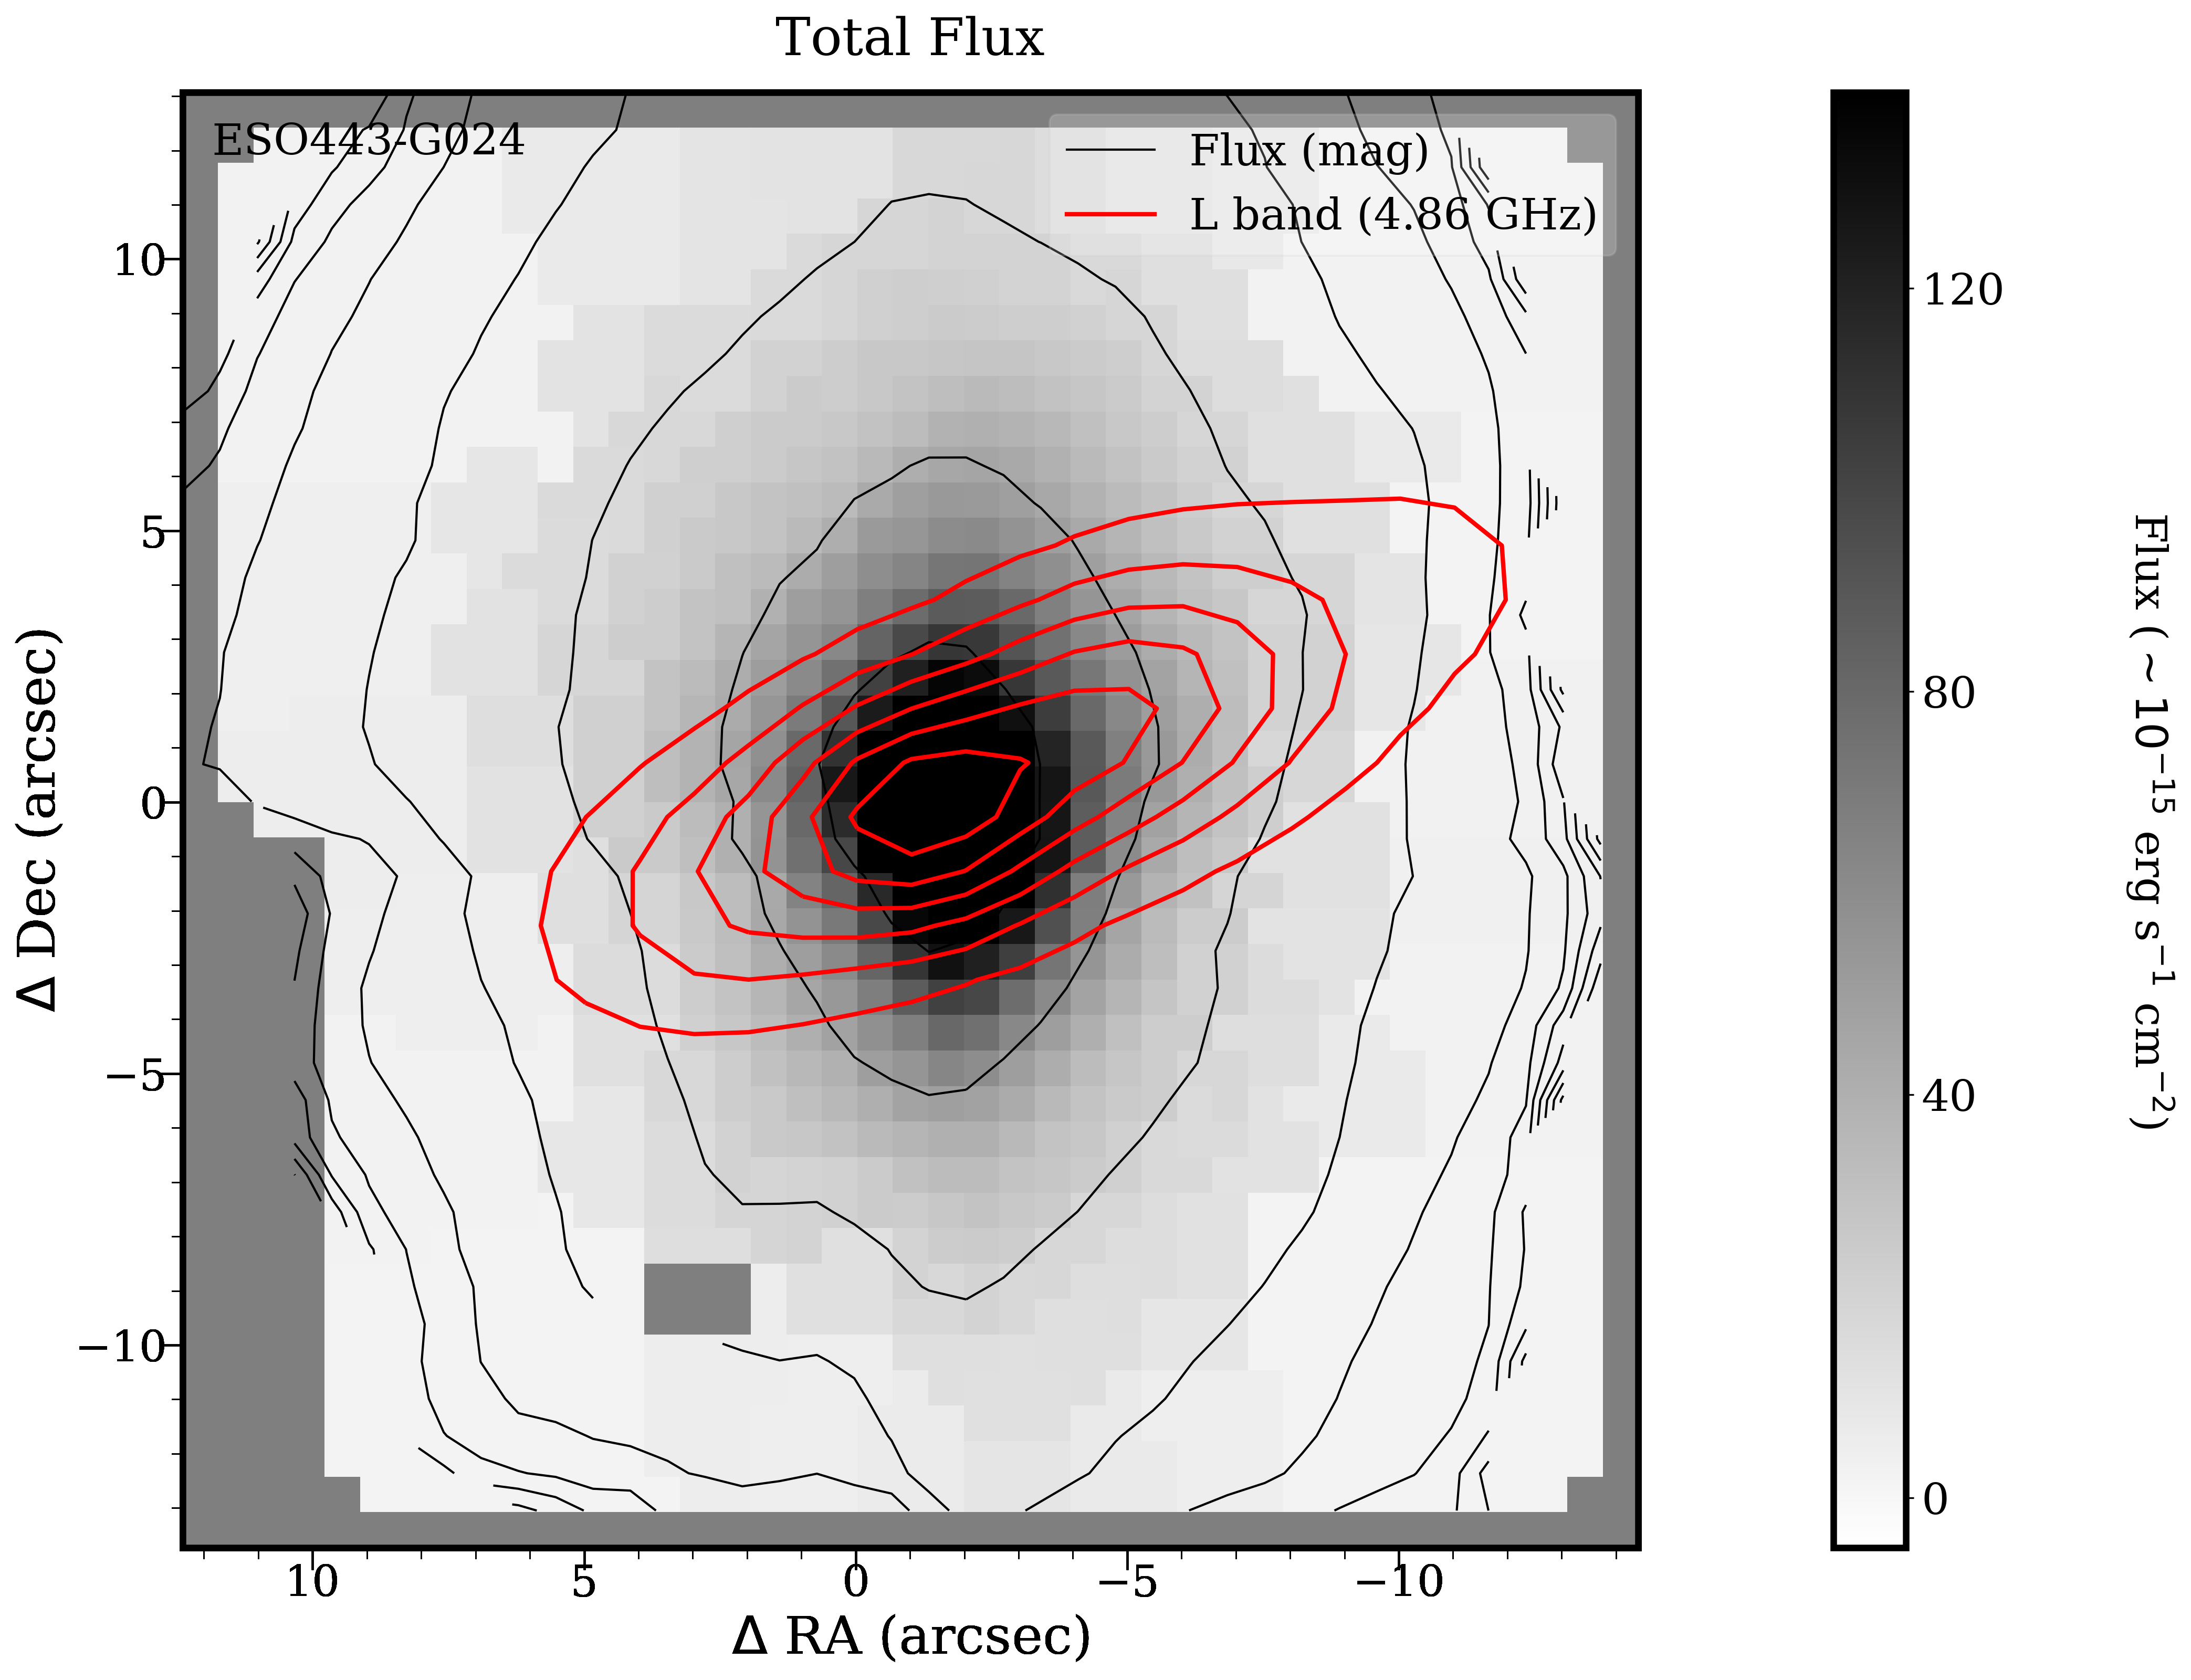
\includegraphics[width=0.245\textwidth]{Vmaps/eso443-g024_stellar_img.png}
      \caption[VIMOS images]{Image for each galaxy in the VIMOS sample. Plots are ordered roughly in peak stellar velocity, with flux contours in black, CO from ALMA in cyan and radio from VLA in red. The radio band displaied is shown in the legend of each plot and depends on what data is avaliable in the archive and which images had a similar resolution and and scale}
      \label{fig:Vstellar_img}
\end{figure*}

\begin{figure*}
      \centering
      \includegraphics[width=0.245\textwidth]{Vmaps/ngc0612_stellar_vel.png}
      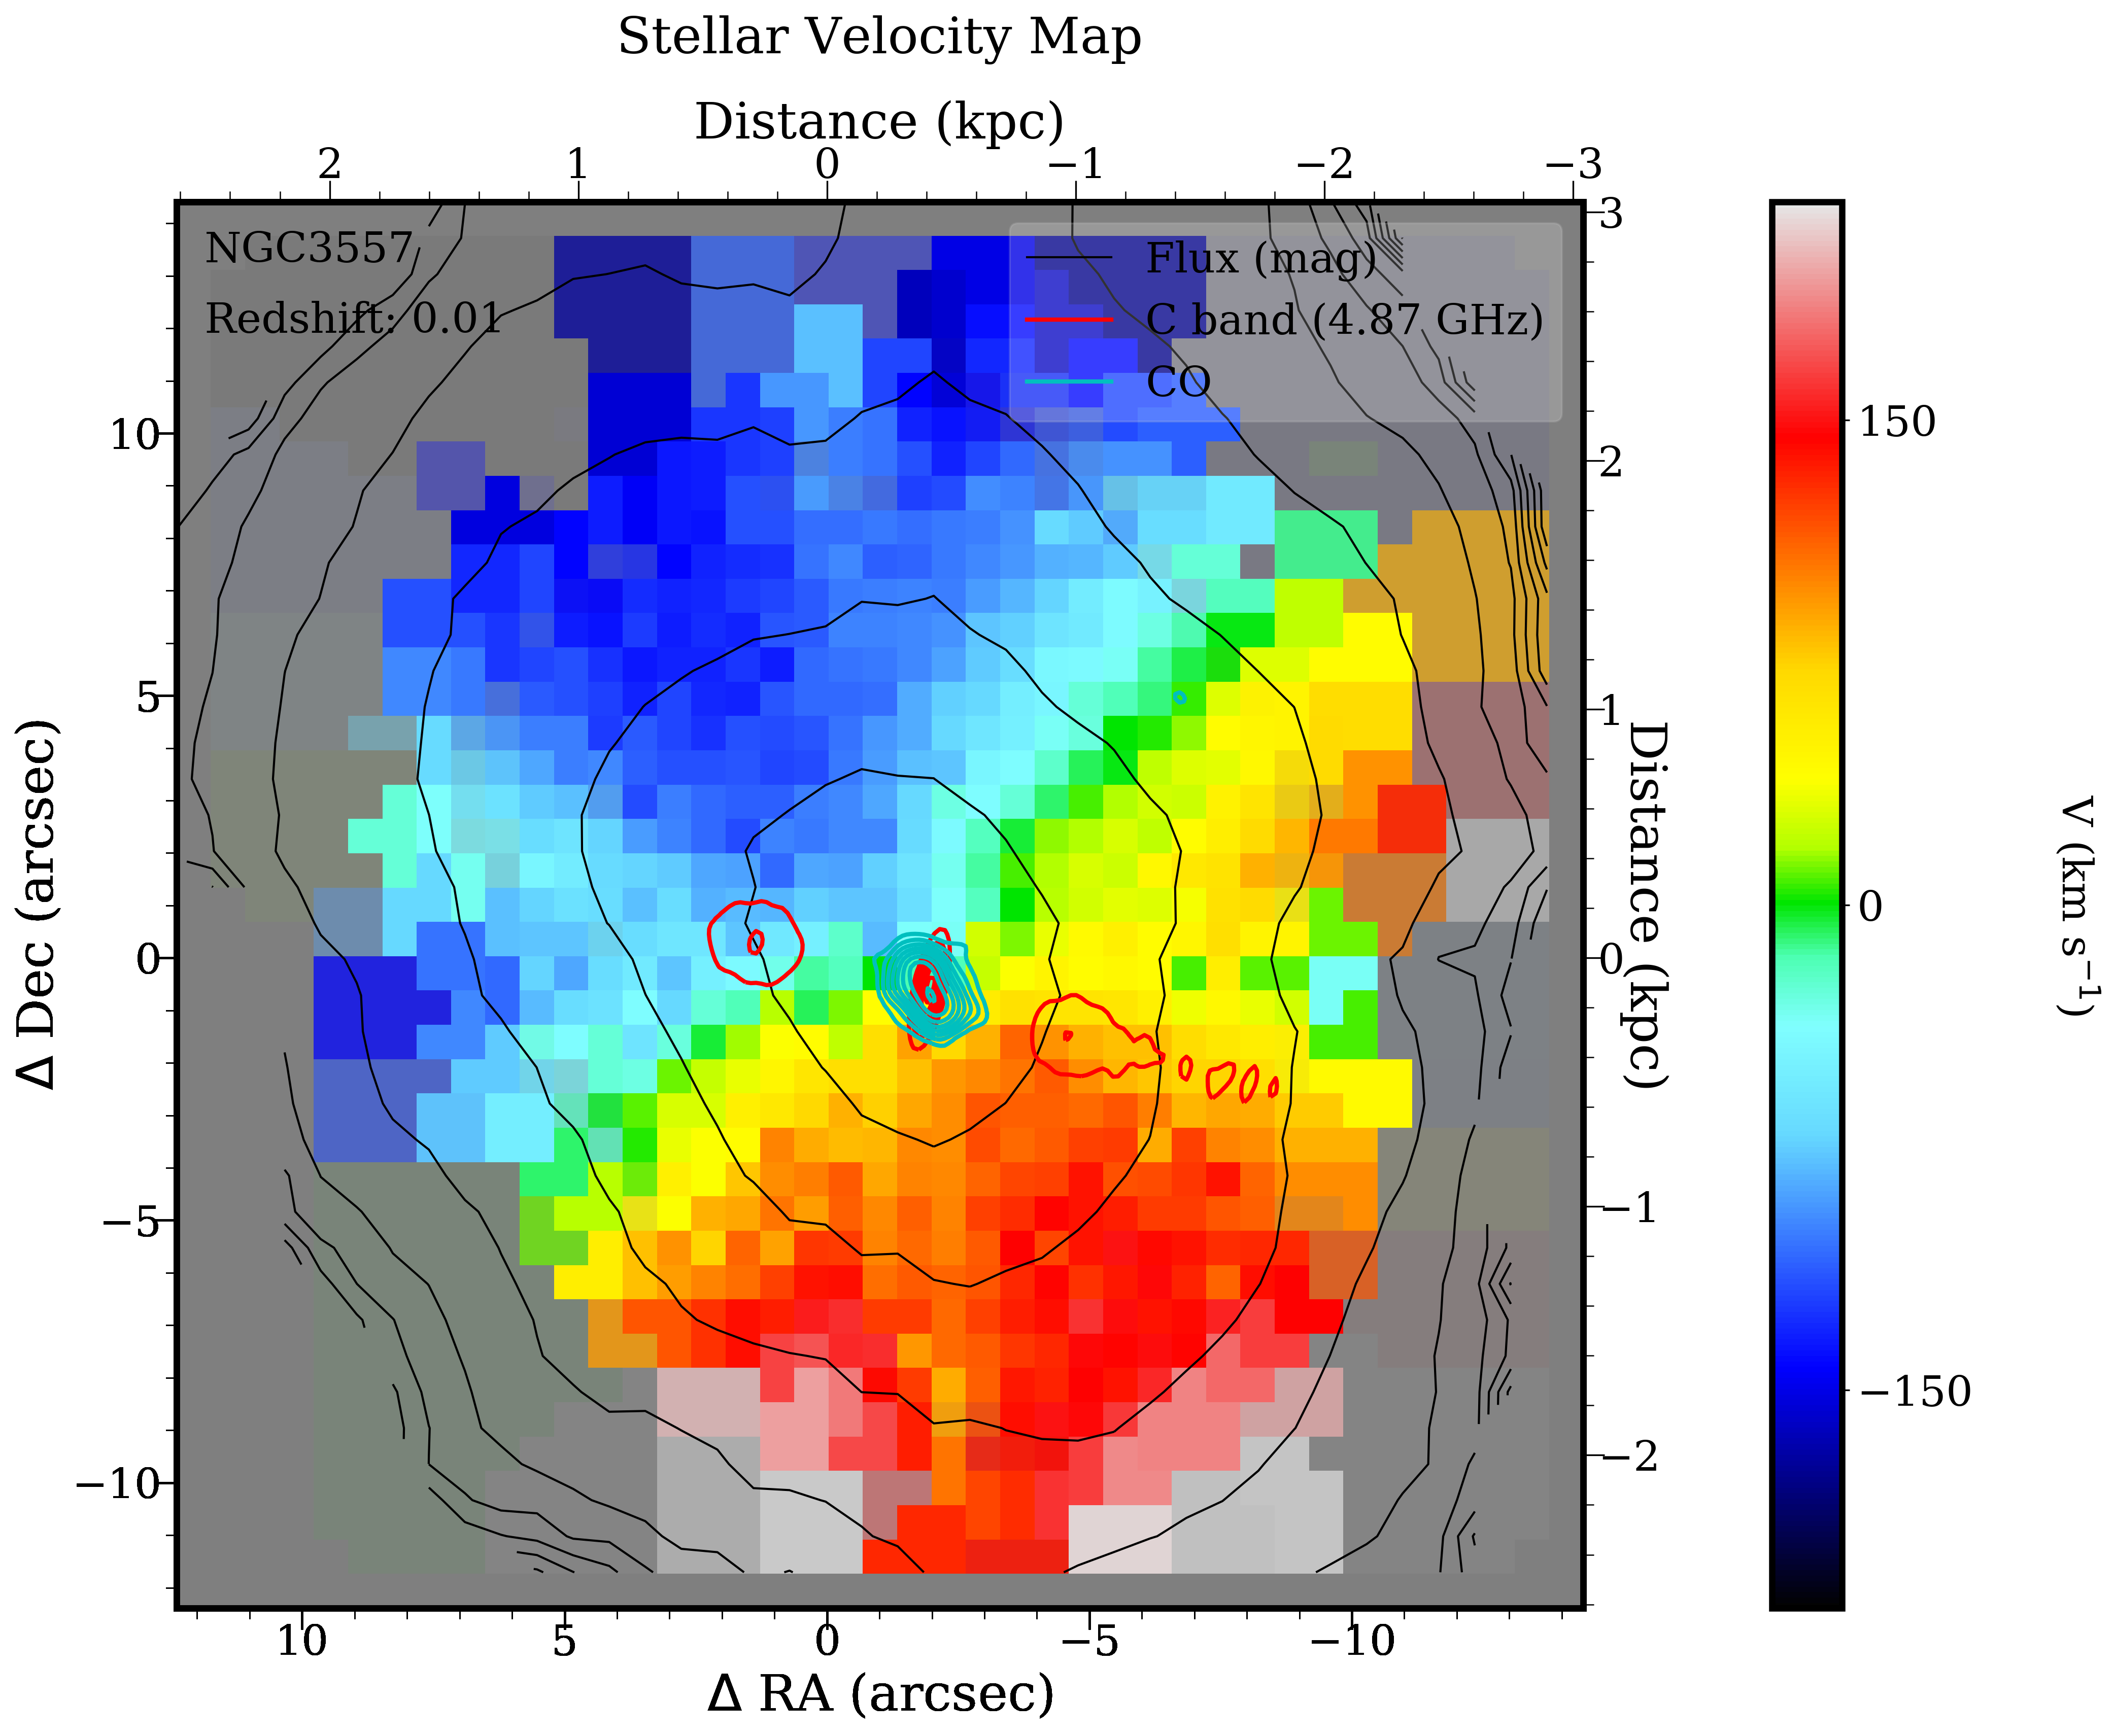
\includegraphics[width=0.245\textwidth]{Vmaps/ngc3557_stellar_vel.png}
      \includegraphics[width=0.245\textwidth]{Vmaps/ngc3100_stellar_vel.png}
      \includegraphics[width=0.245\textwidth]{Vmaps/ic1459_stellar_vel.png}
      \includegraphics[width=0.245\textwidth]{Vmaps/pks0718-34_stellar_vel.png}
      \includegraphics[width=0.245\textwidth]{Vmaps/ic4296_stellar_vel.png}
      \includegraphics[width=0.245\textwidth]{Vmaps/ngc7075_stellar_vel.png}
      \includegraphics[width=0.245\textwidth]{Vmaps/ic1531_stellar_vel.png}
      \includegraphics[width=0.245\textwidth]{Vmaps/ngc1399_stellar_vel.png}
      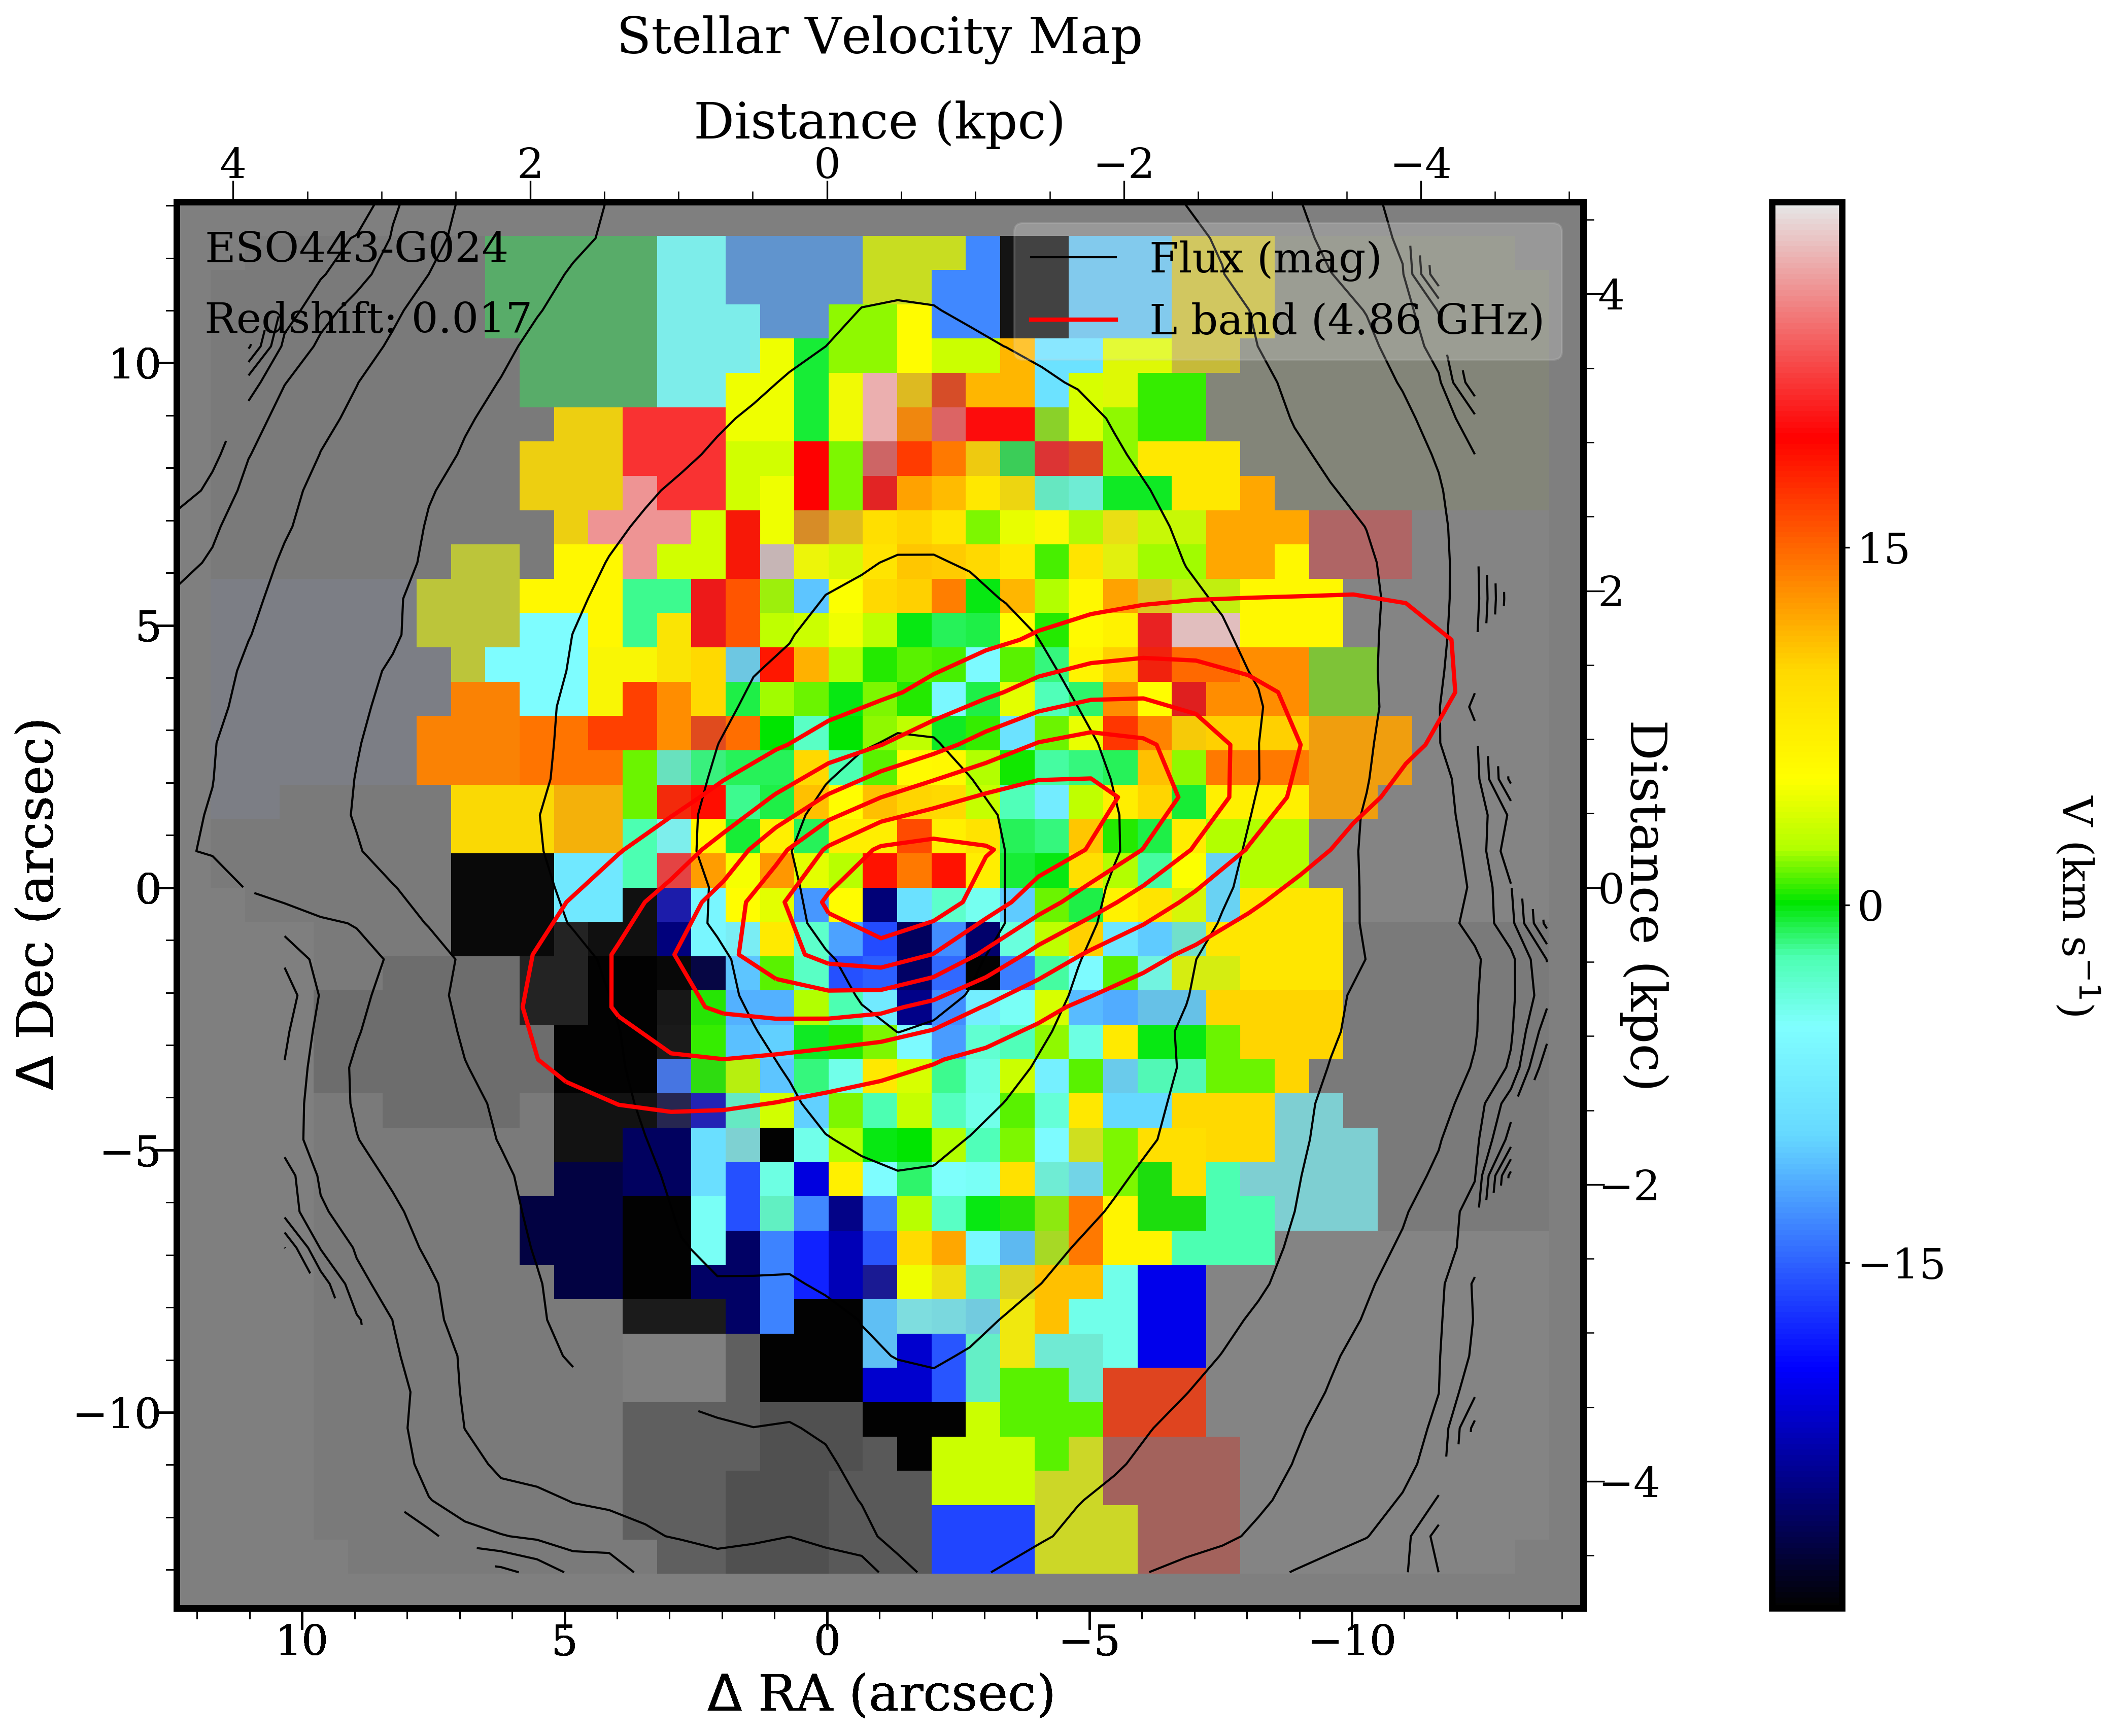
\includegraphics[width=0.245\textwidth]{Vmaps/eso443-g024_stellar_vel.png}
      \caption[VIMOS velocity maps]{Velocity for each galaxy in the VIMOS sample. Plots are ordered and contour colors are as in figure \ref{fig:Vstellar_img}}
      \label{fig:Vstellar_vel}
\end{figure*}

\begin{figure*}
      \centering
      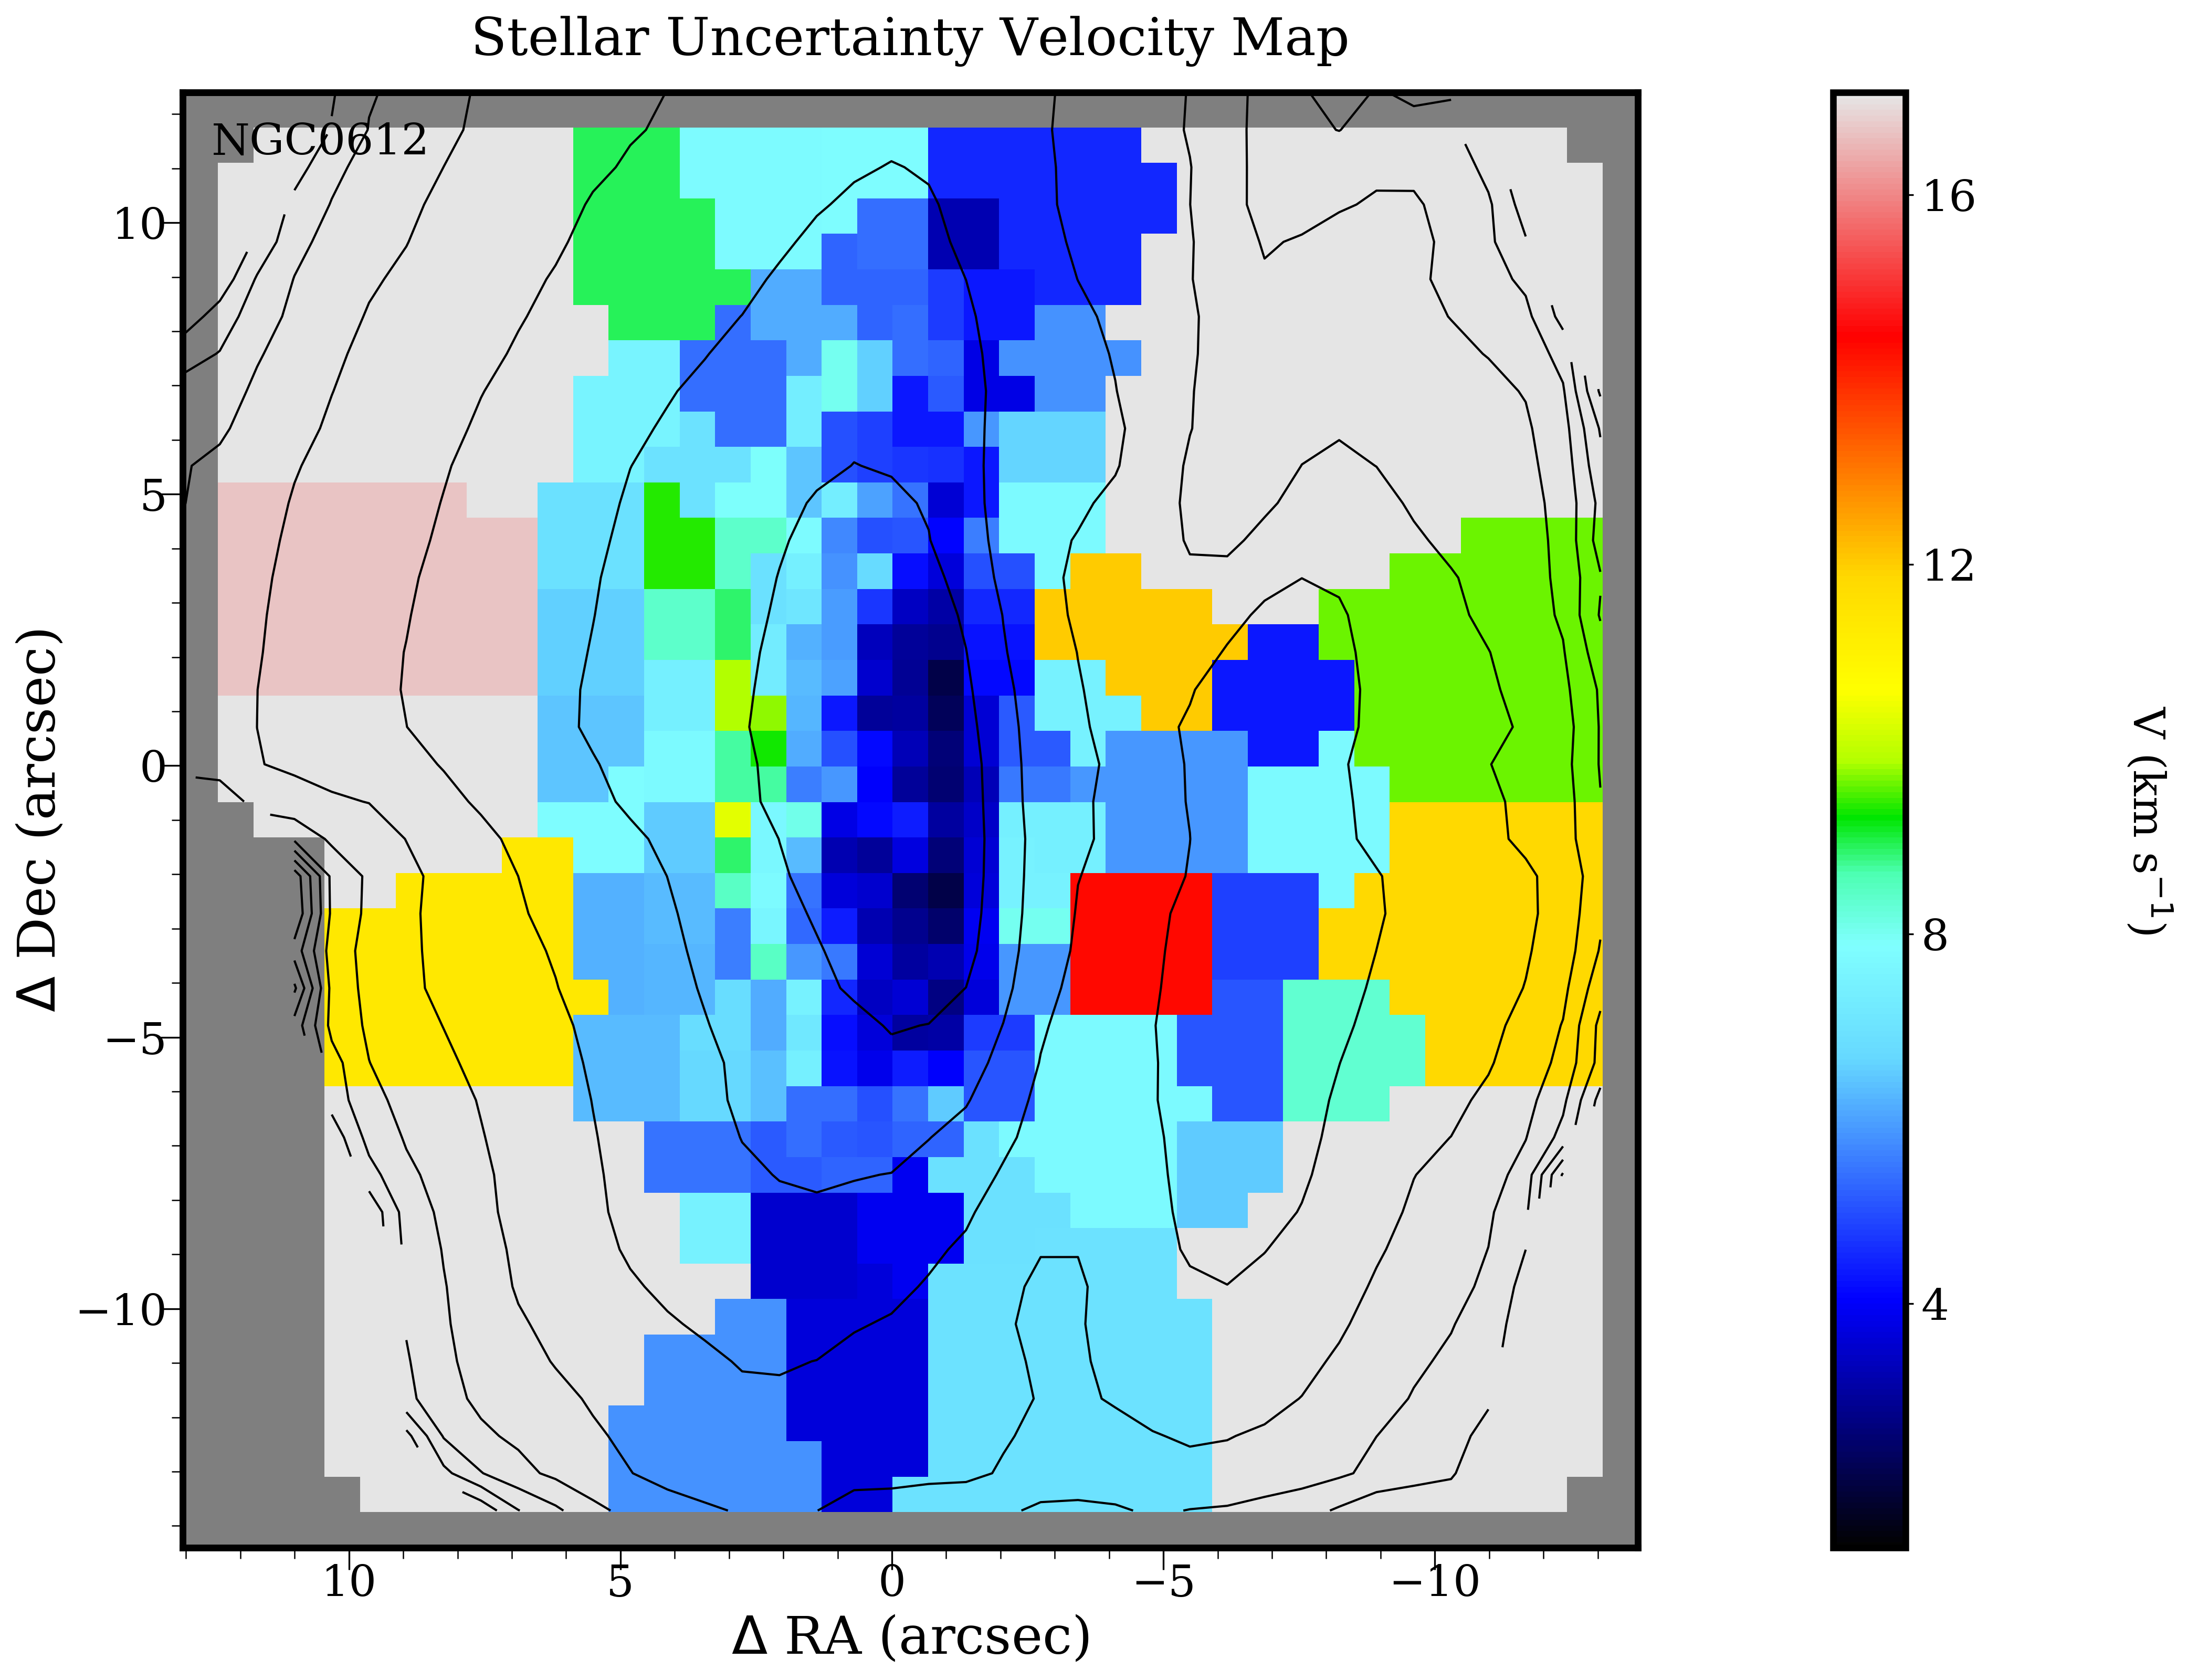
\includegraphics[width=0.245\textwidth]{Vmaps/ngc0612_stellar_vel_uncert.png}
      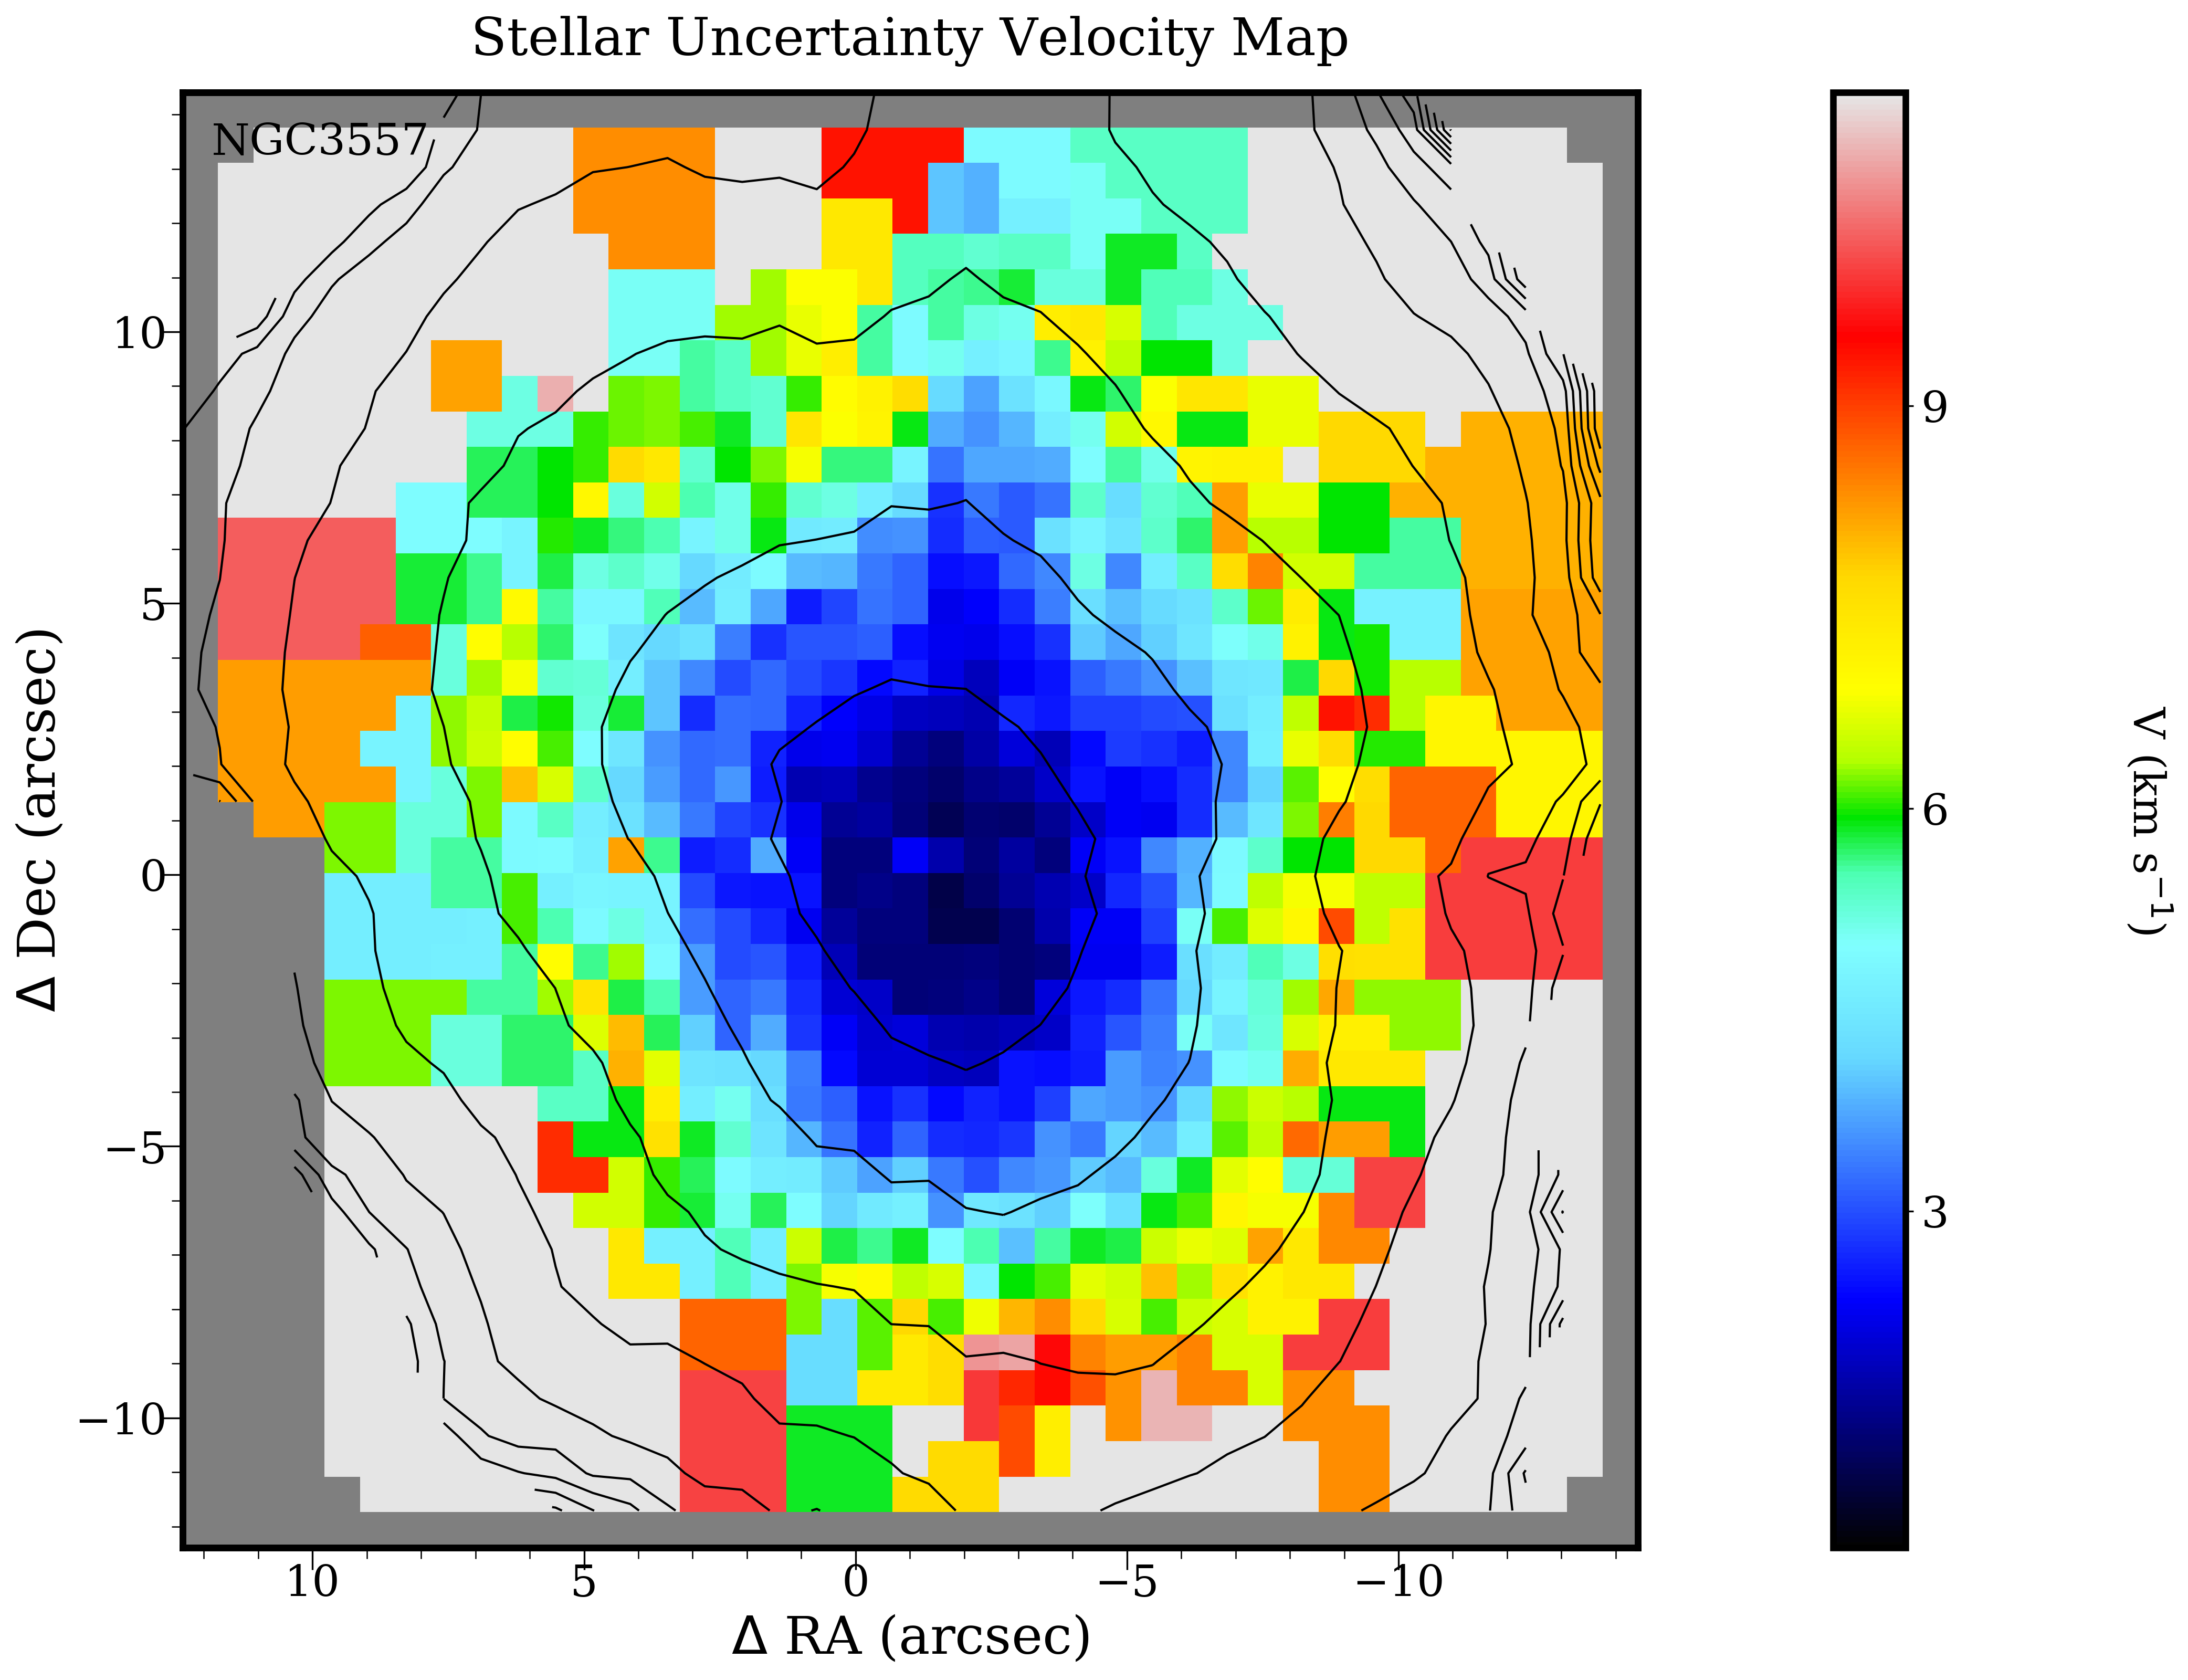
\includegraphics[width=0.245\textwidth]{Vmaps/ngc3557_stellar_vel_uncert.png}
      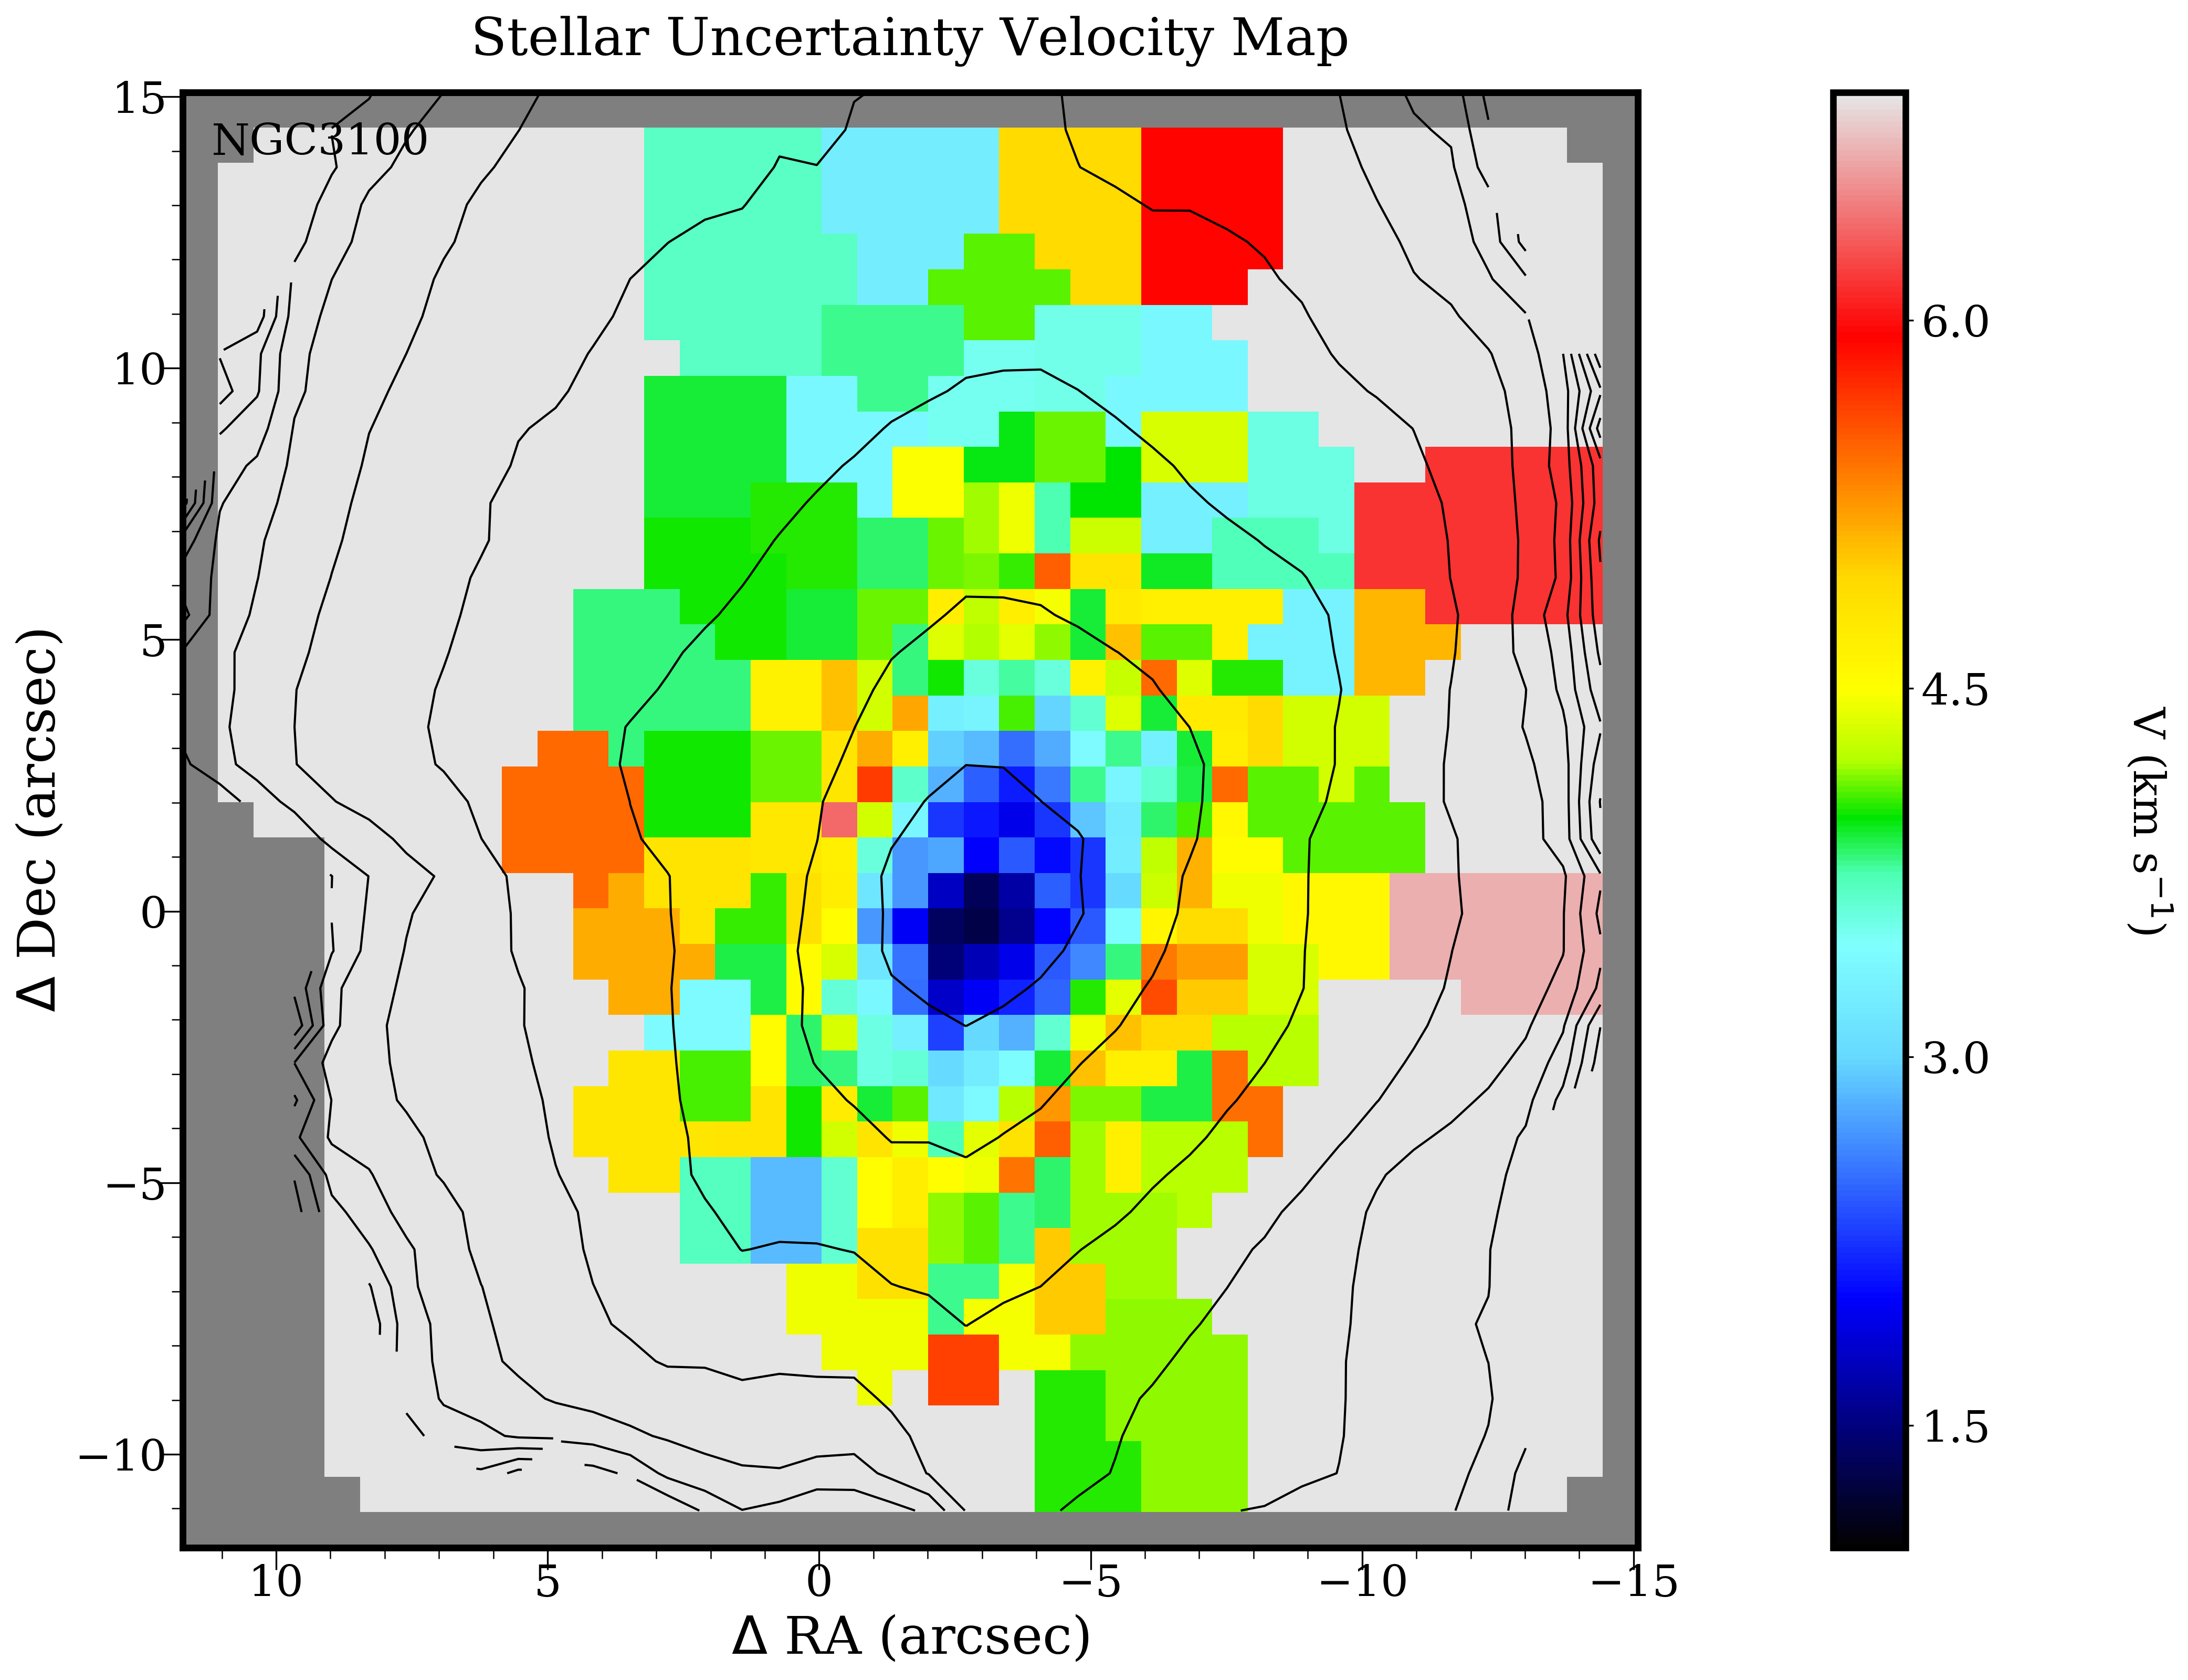
\includegraphics[width=0.245\textwidth]{Vmaps/ngc3100_stellar_vel_uncert.png}
      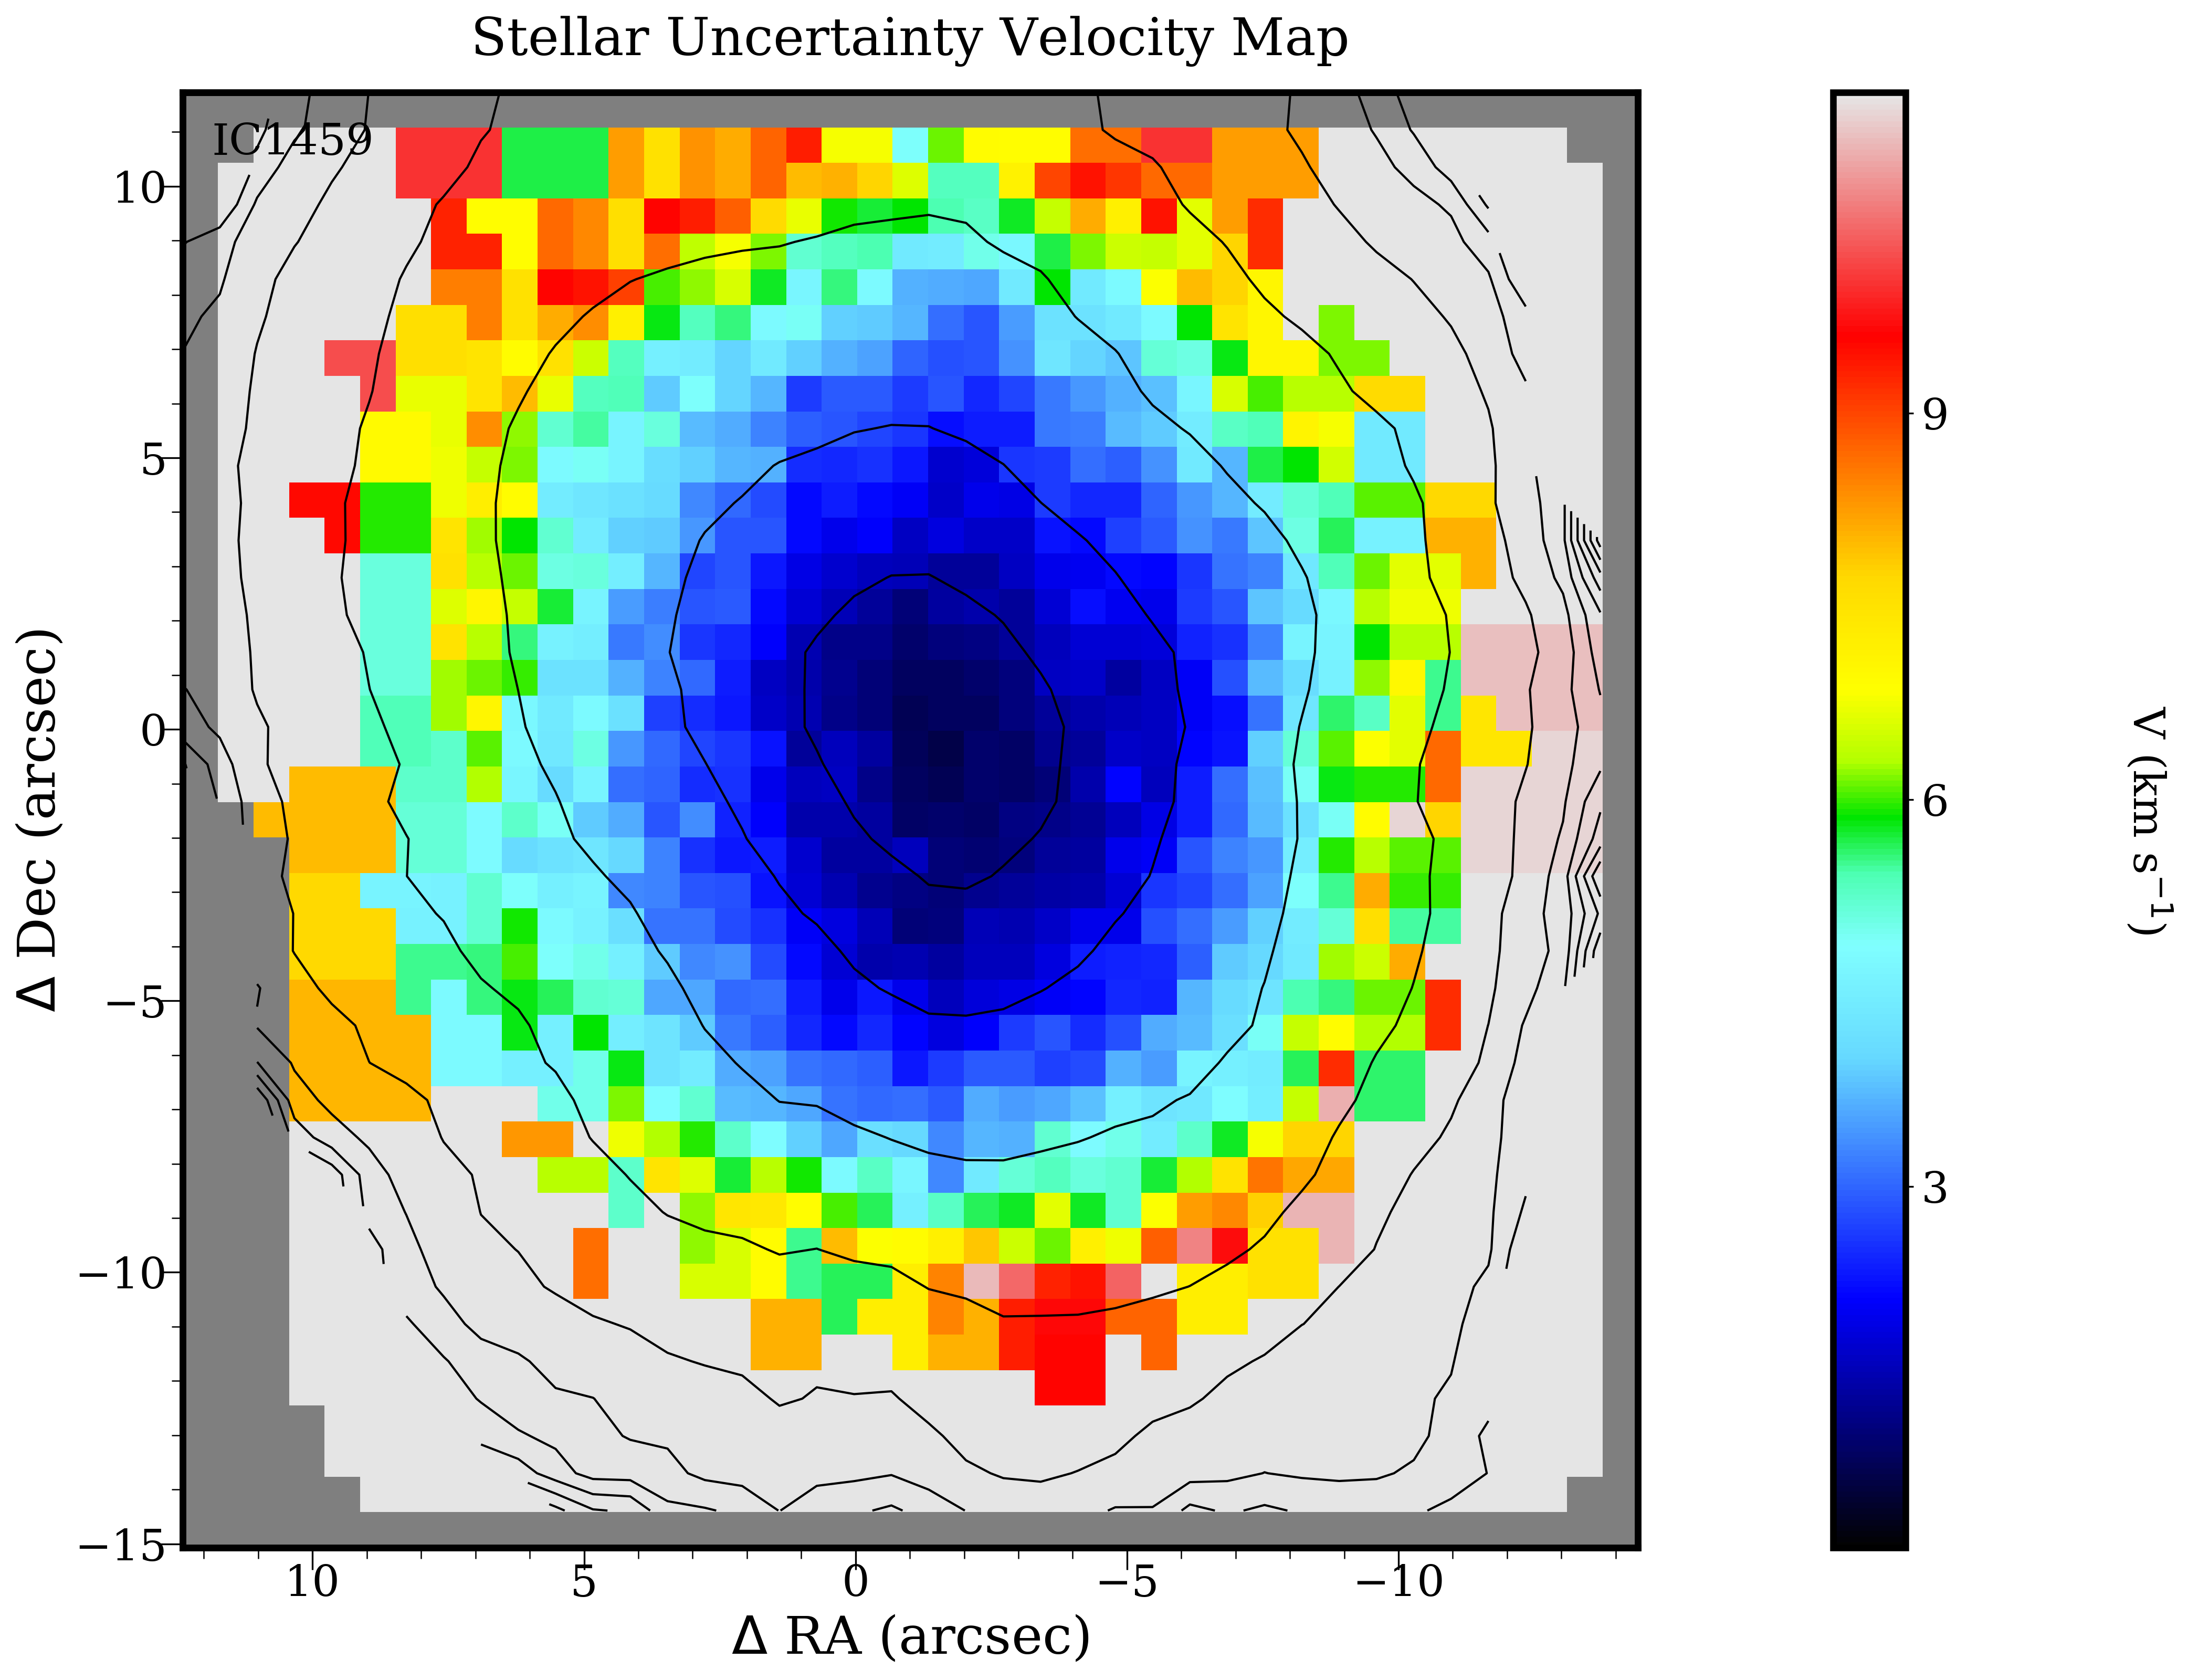
\includegraphics[width=0.245\textwidth]{Vmaps/ic1459_stellar_vel_uncert.png}
      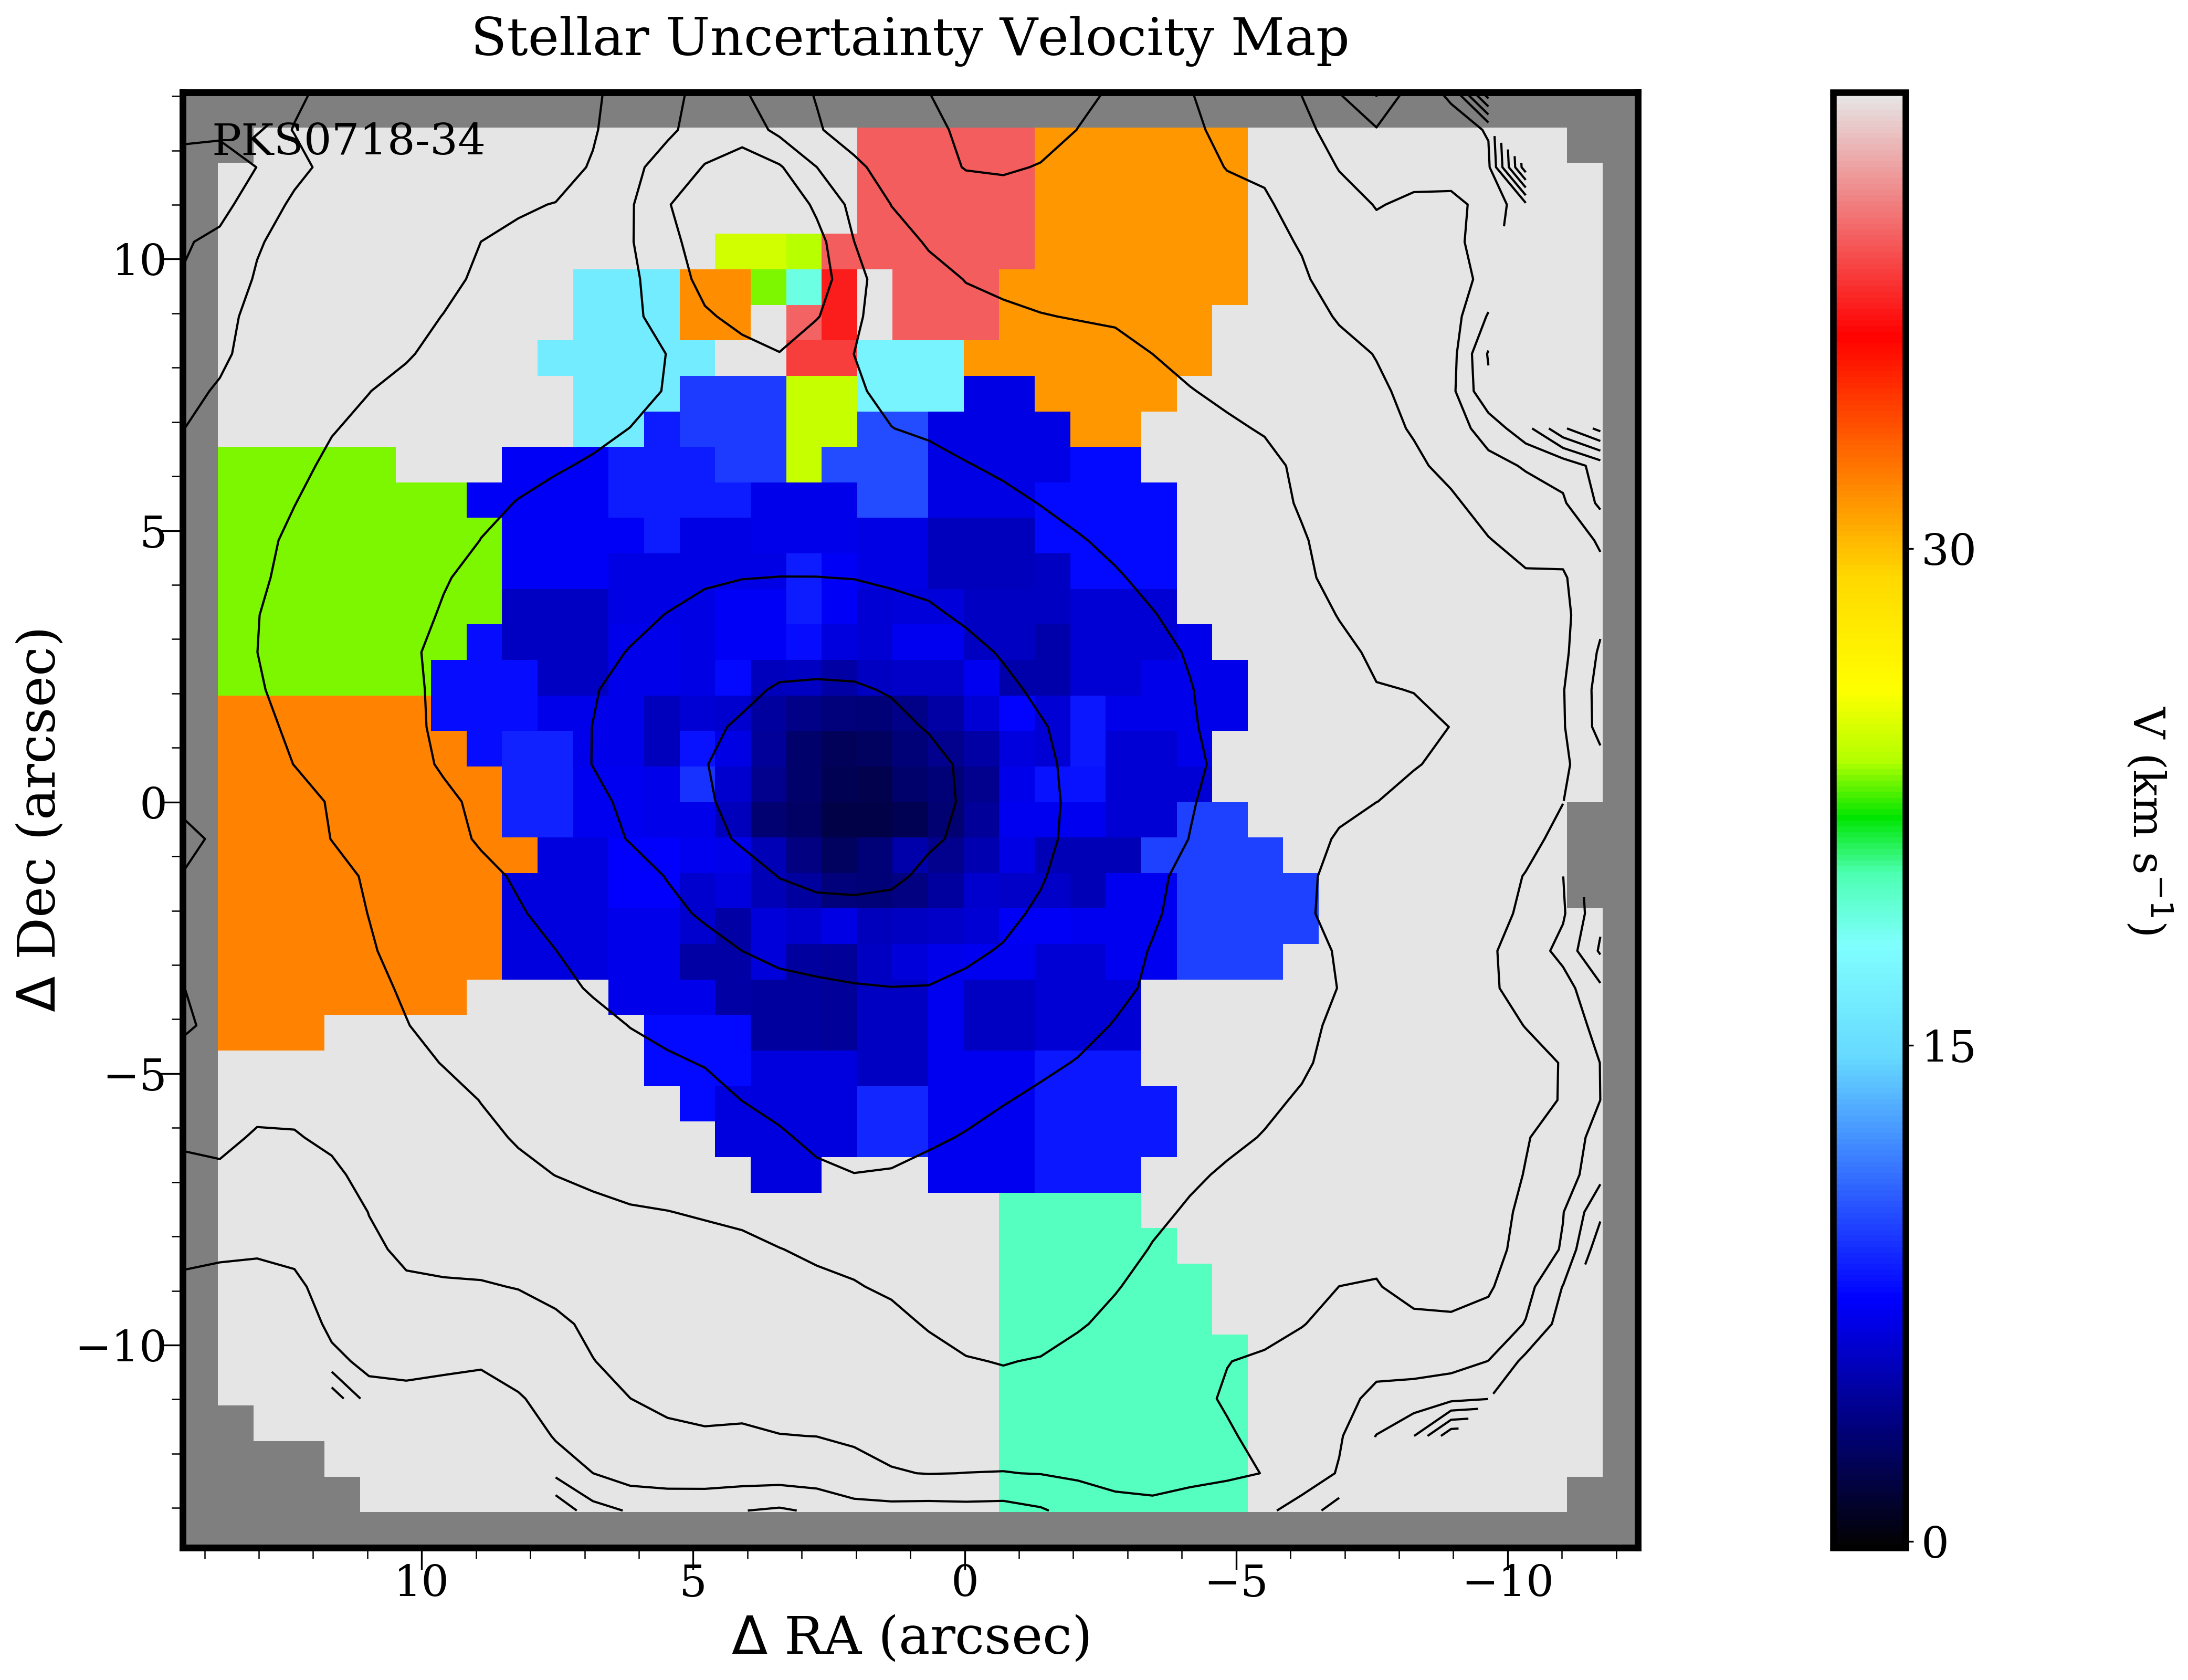
\includegraphics[width=0.245\textwidth]{Vmaps/pks0718-34_stellar_vel_uncert.png}
      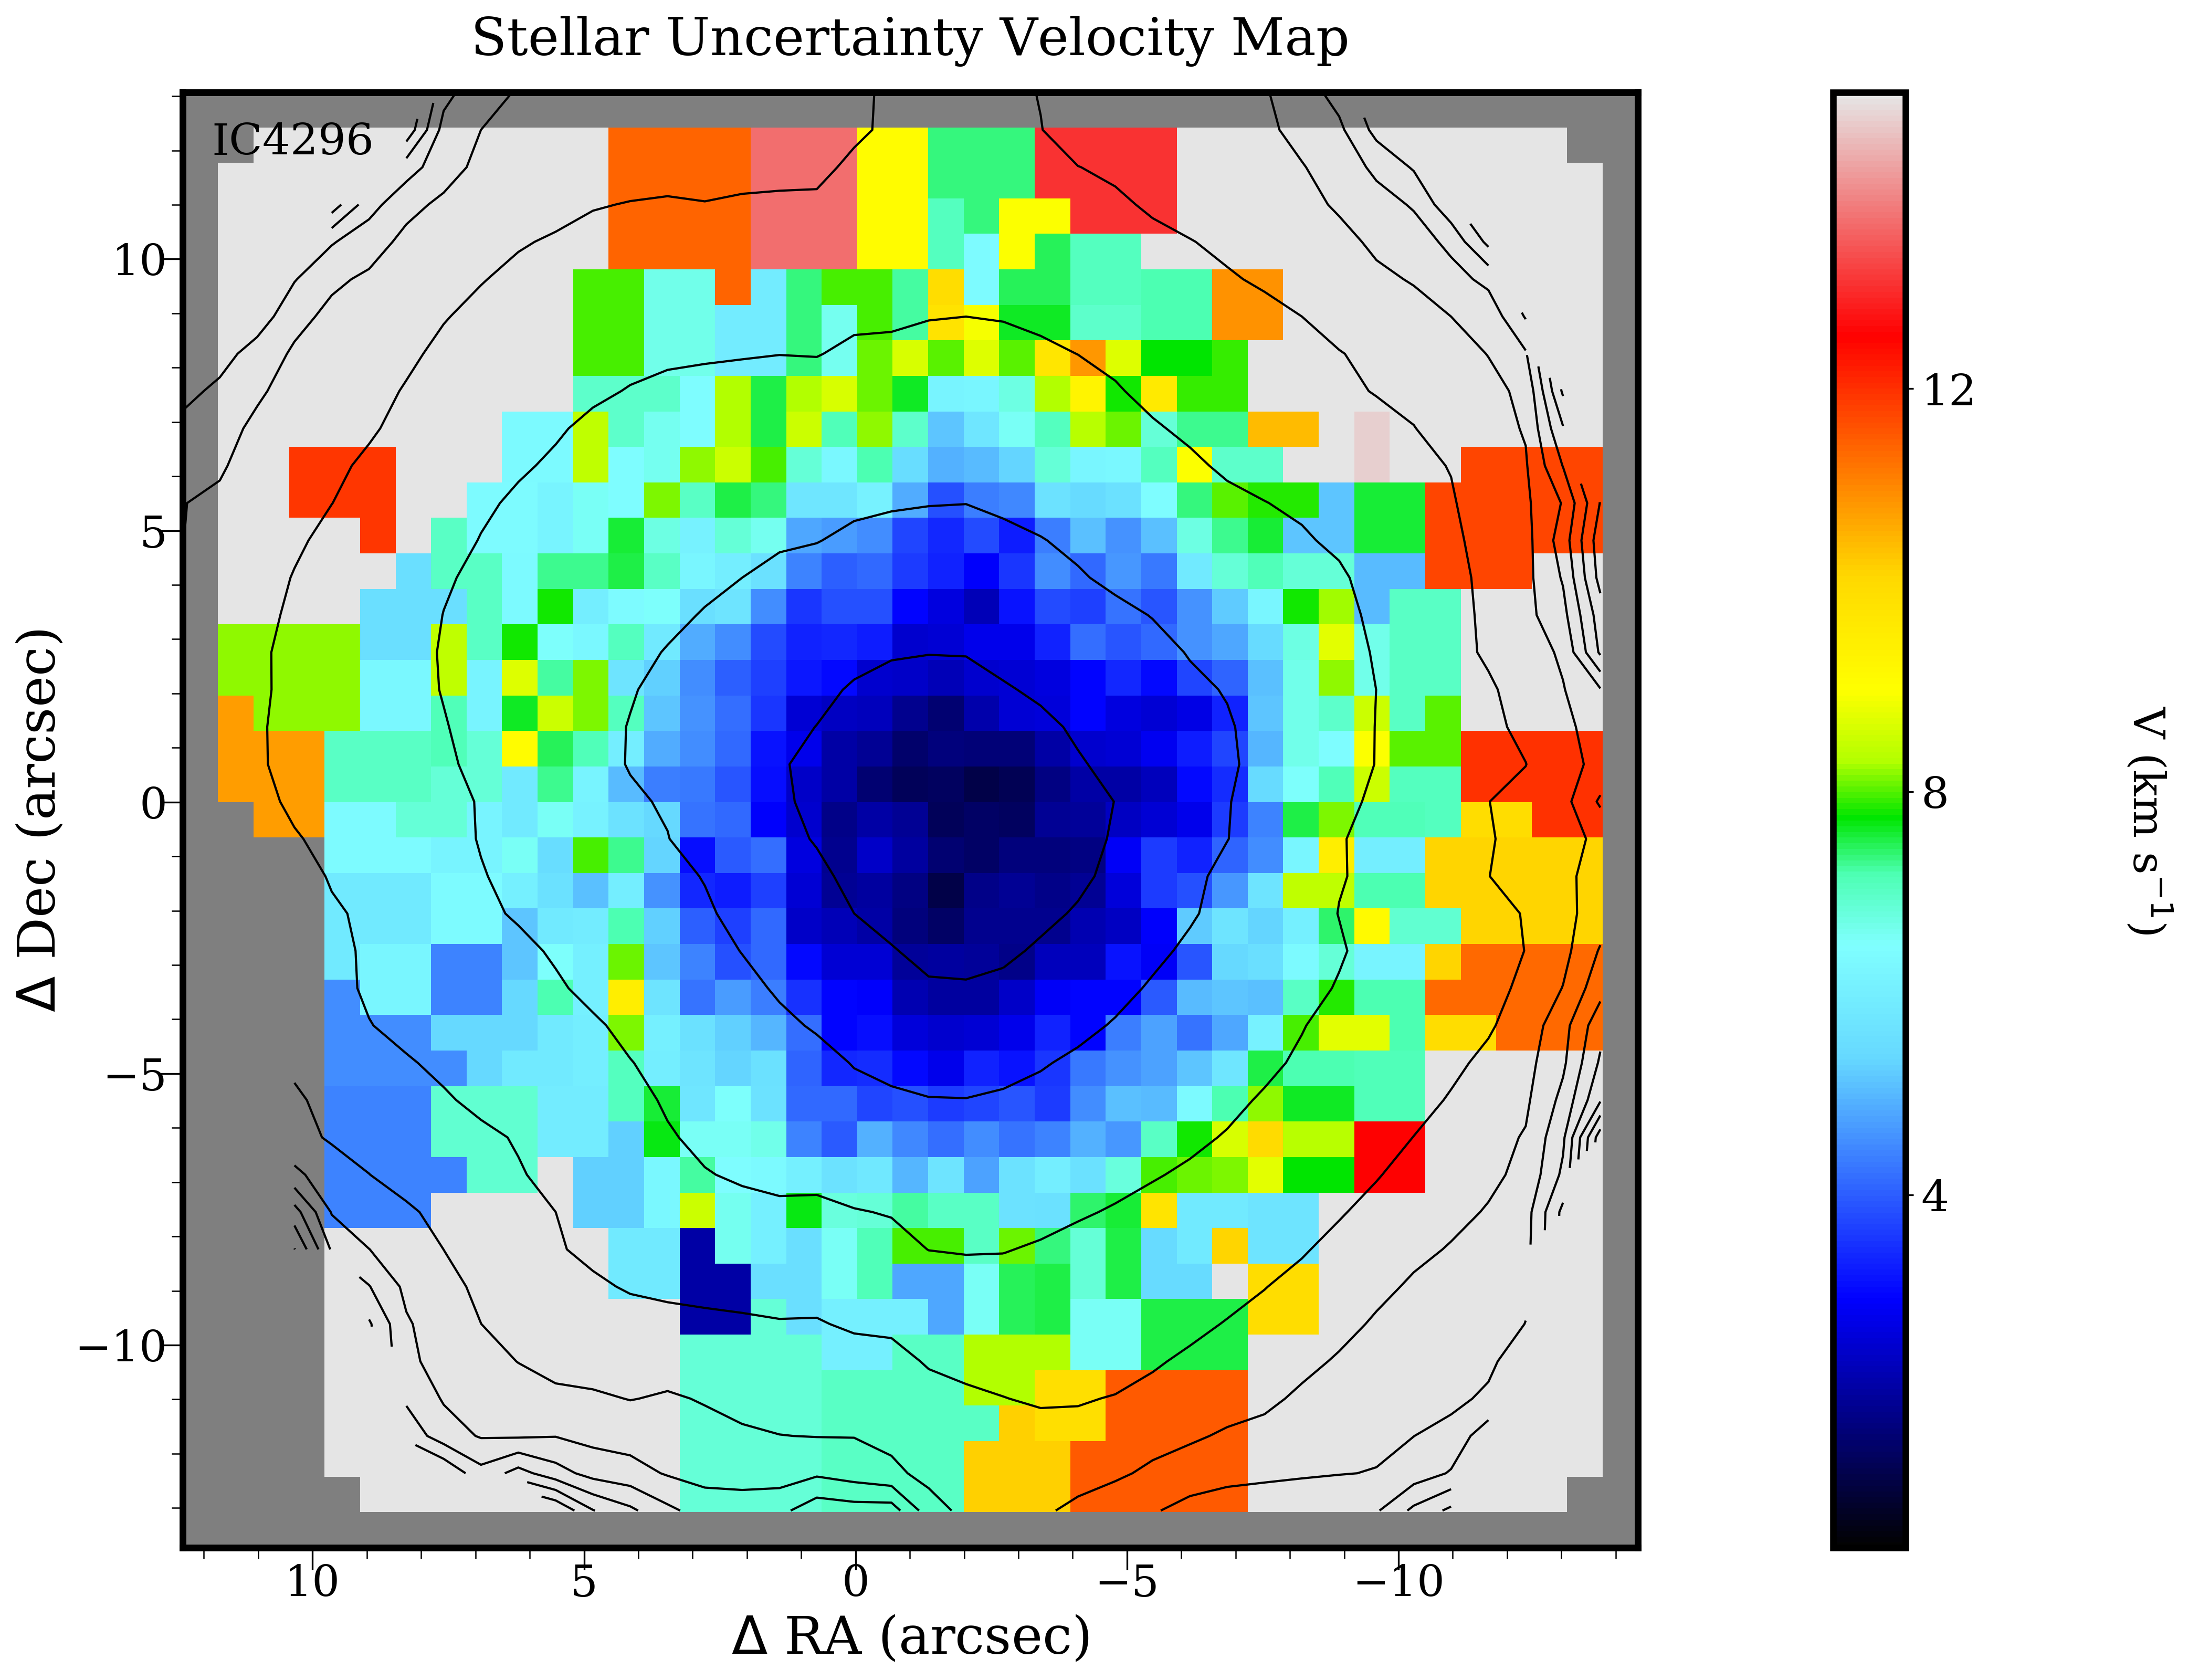
\includegraphics[width=0.245\textwidth]{Vmaps/ic4296_stellar_vel_uncert.png}
      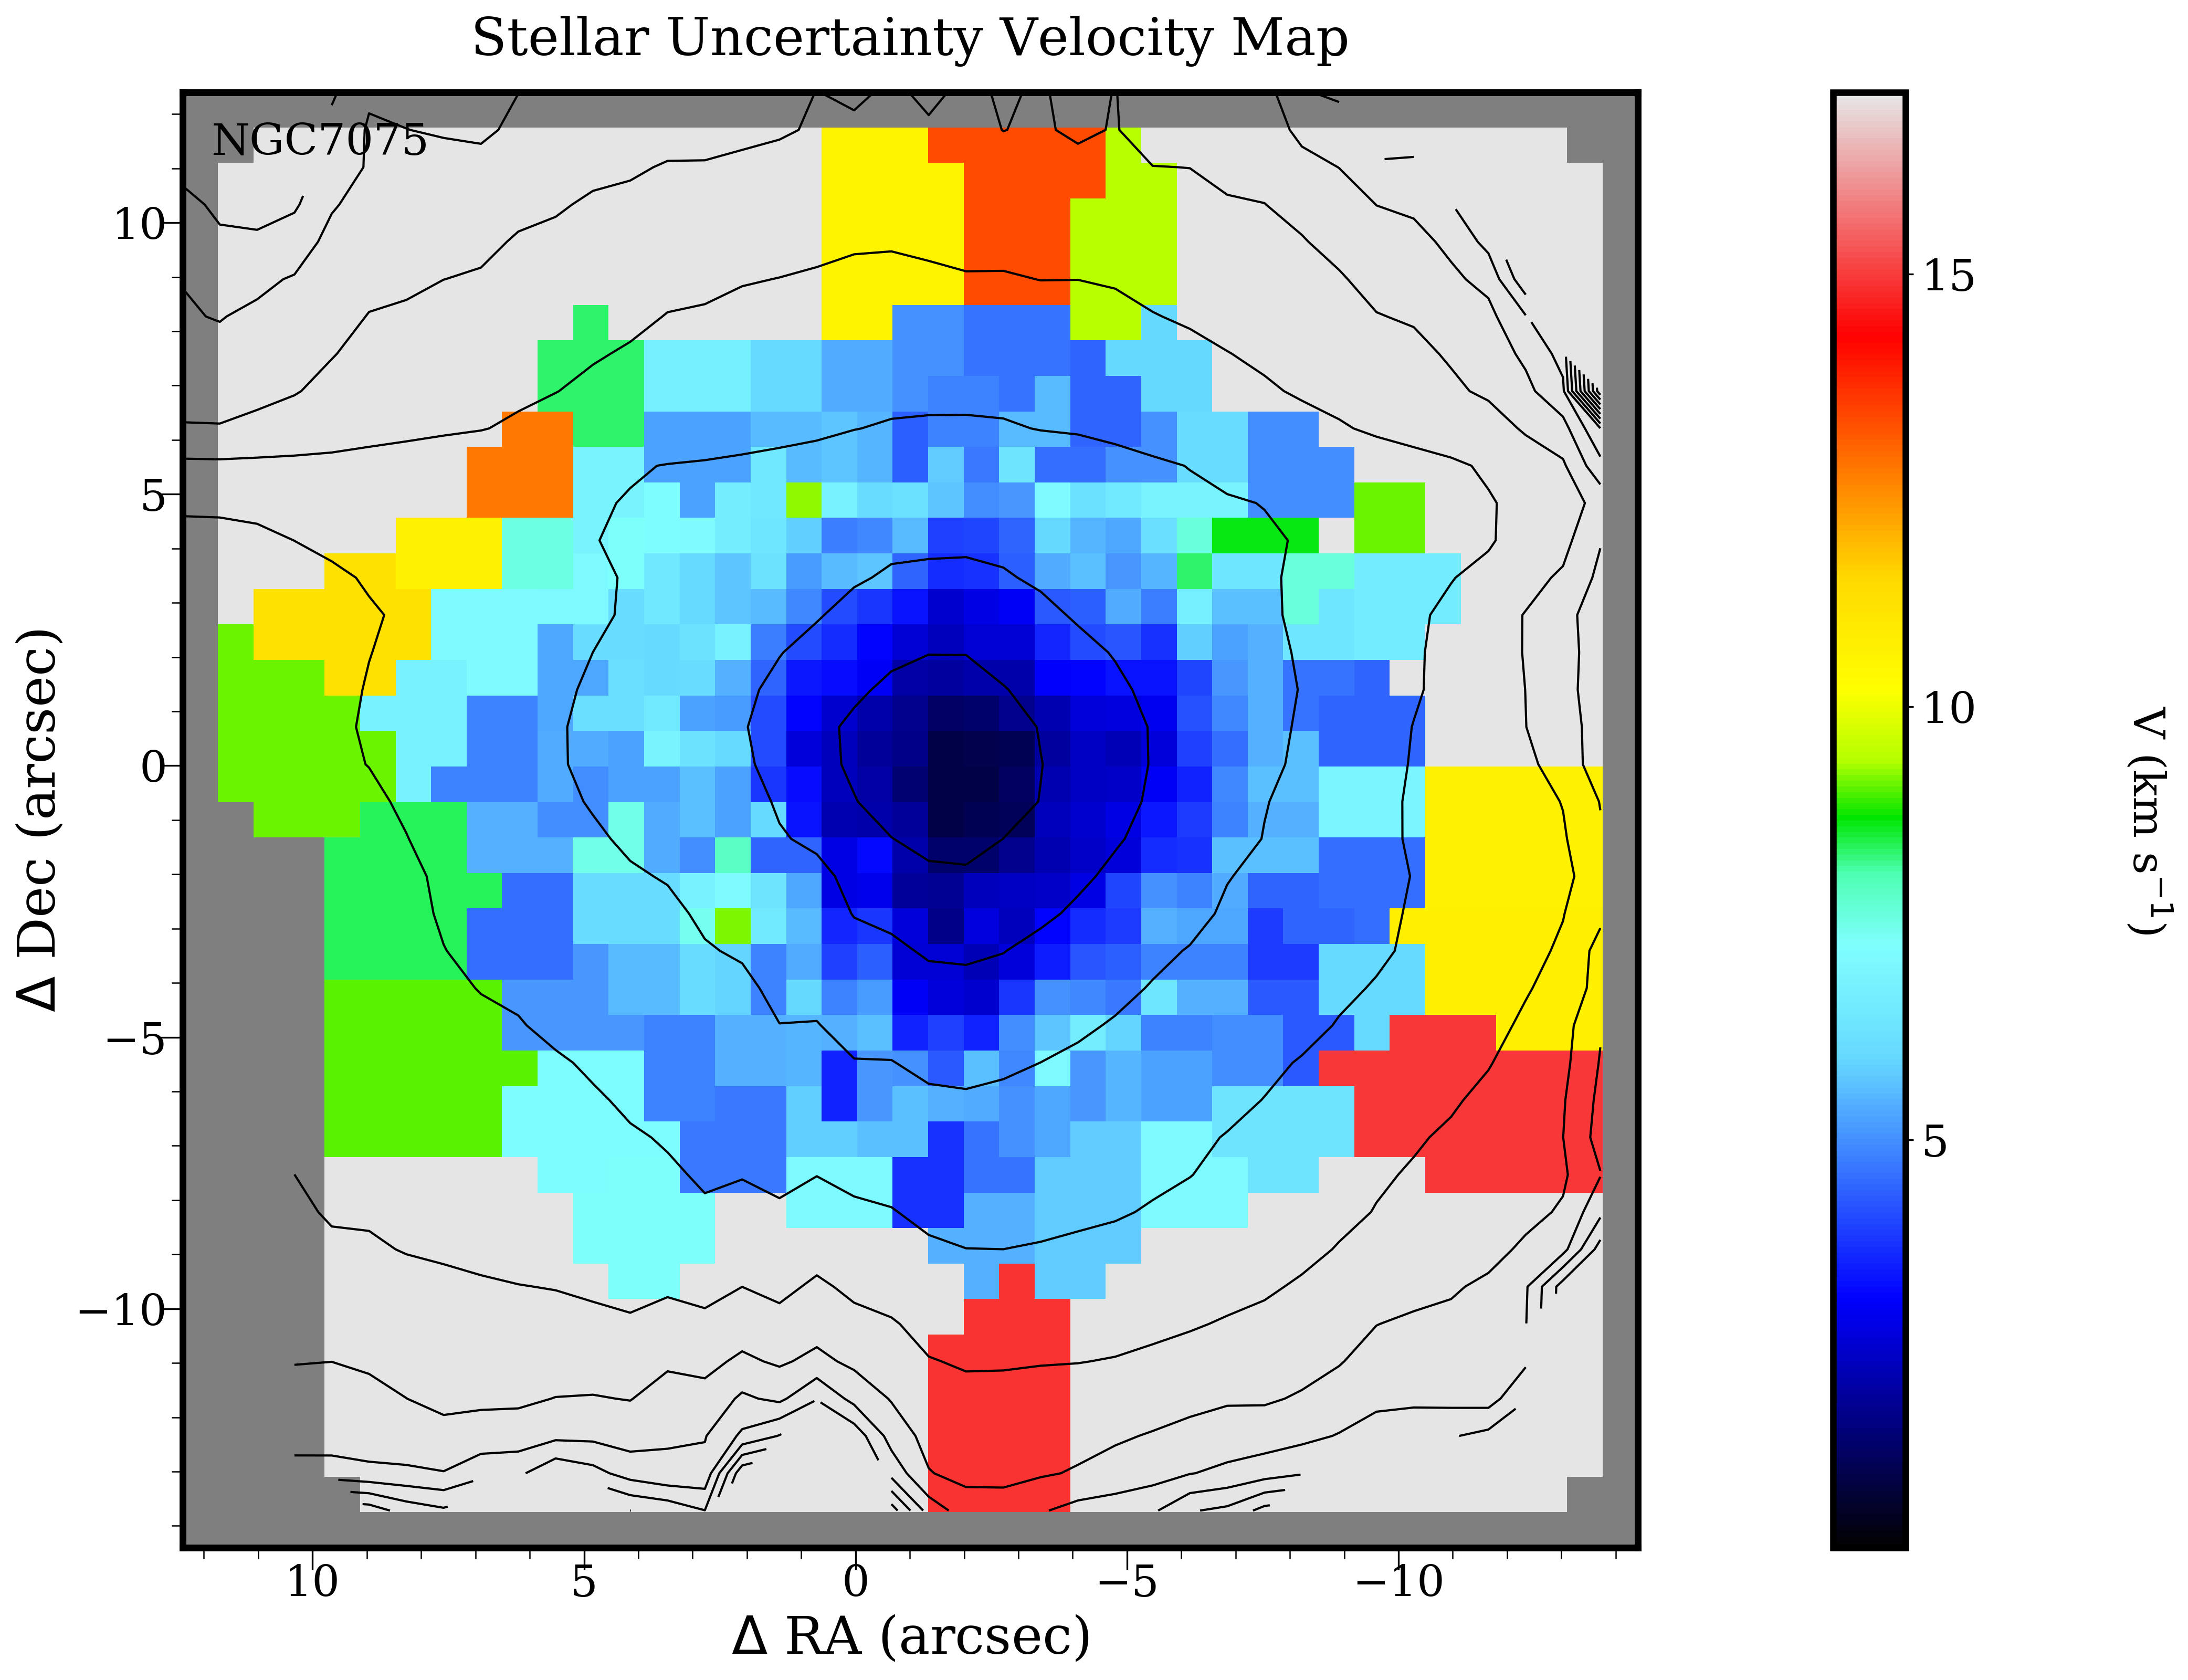
\includegraphics[width=0.245\textwidth]{Vmaps/ngc7075_stellar_vel_uncert.png}
      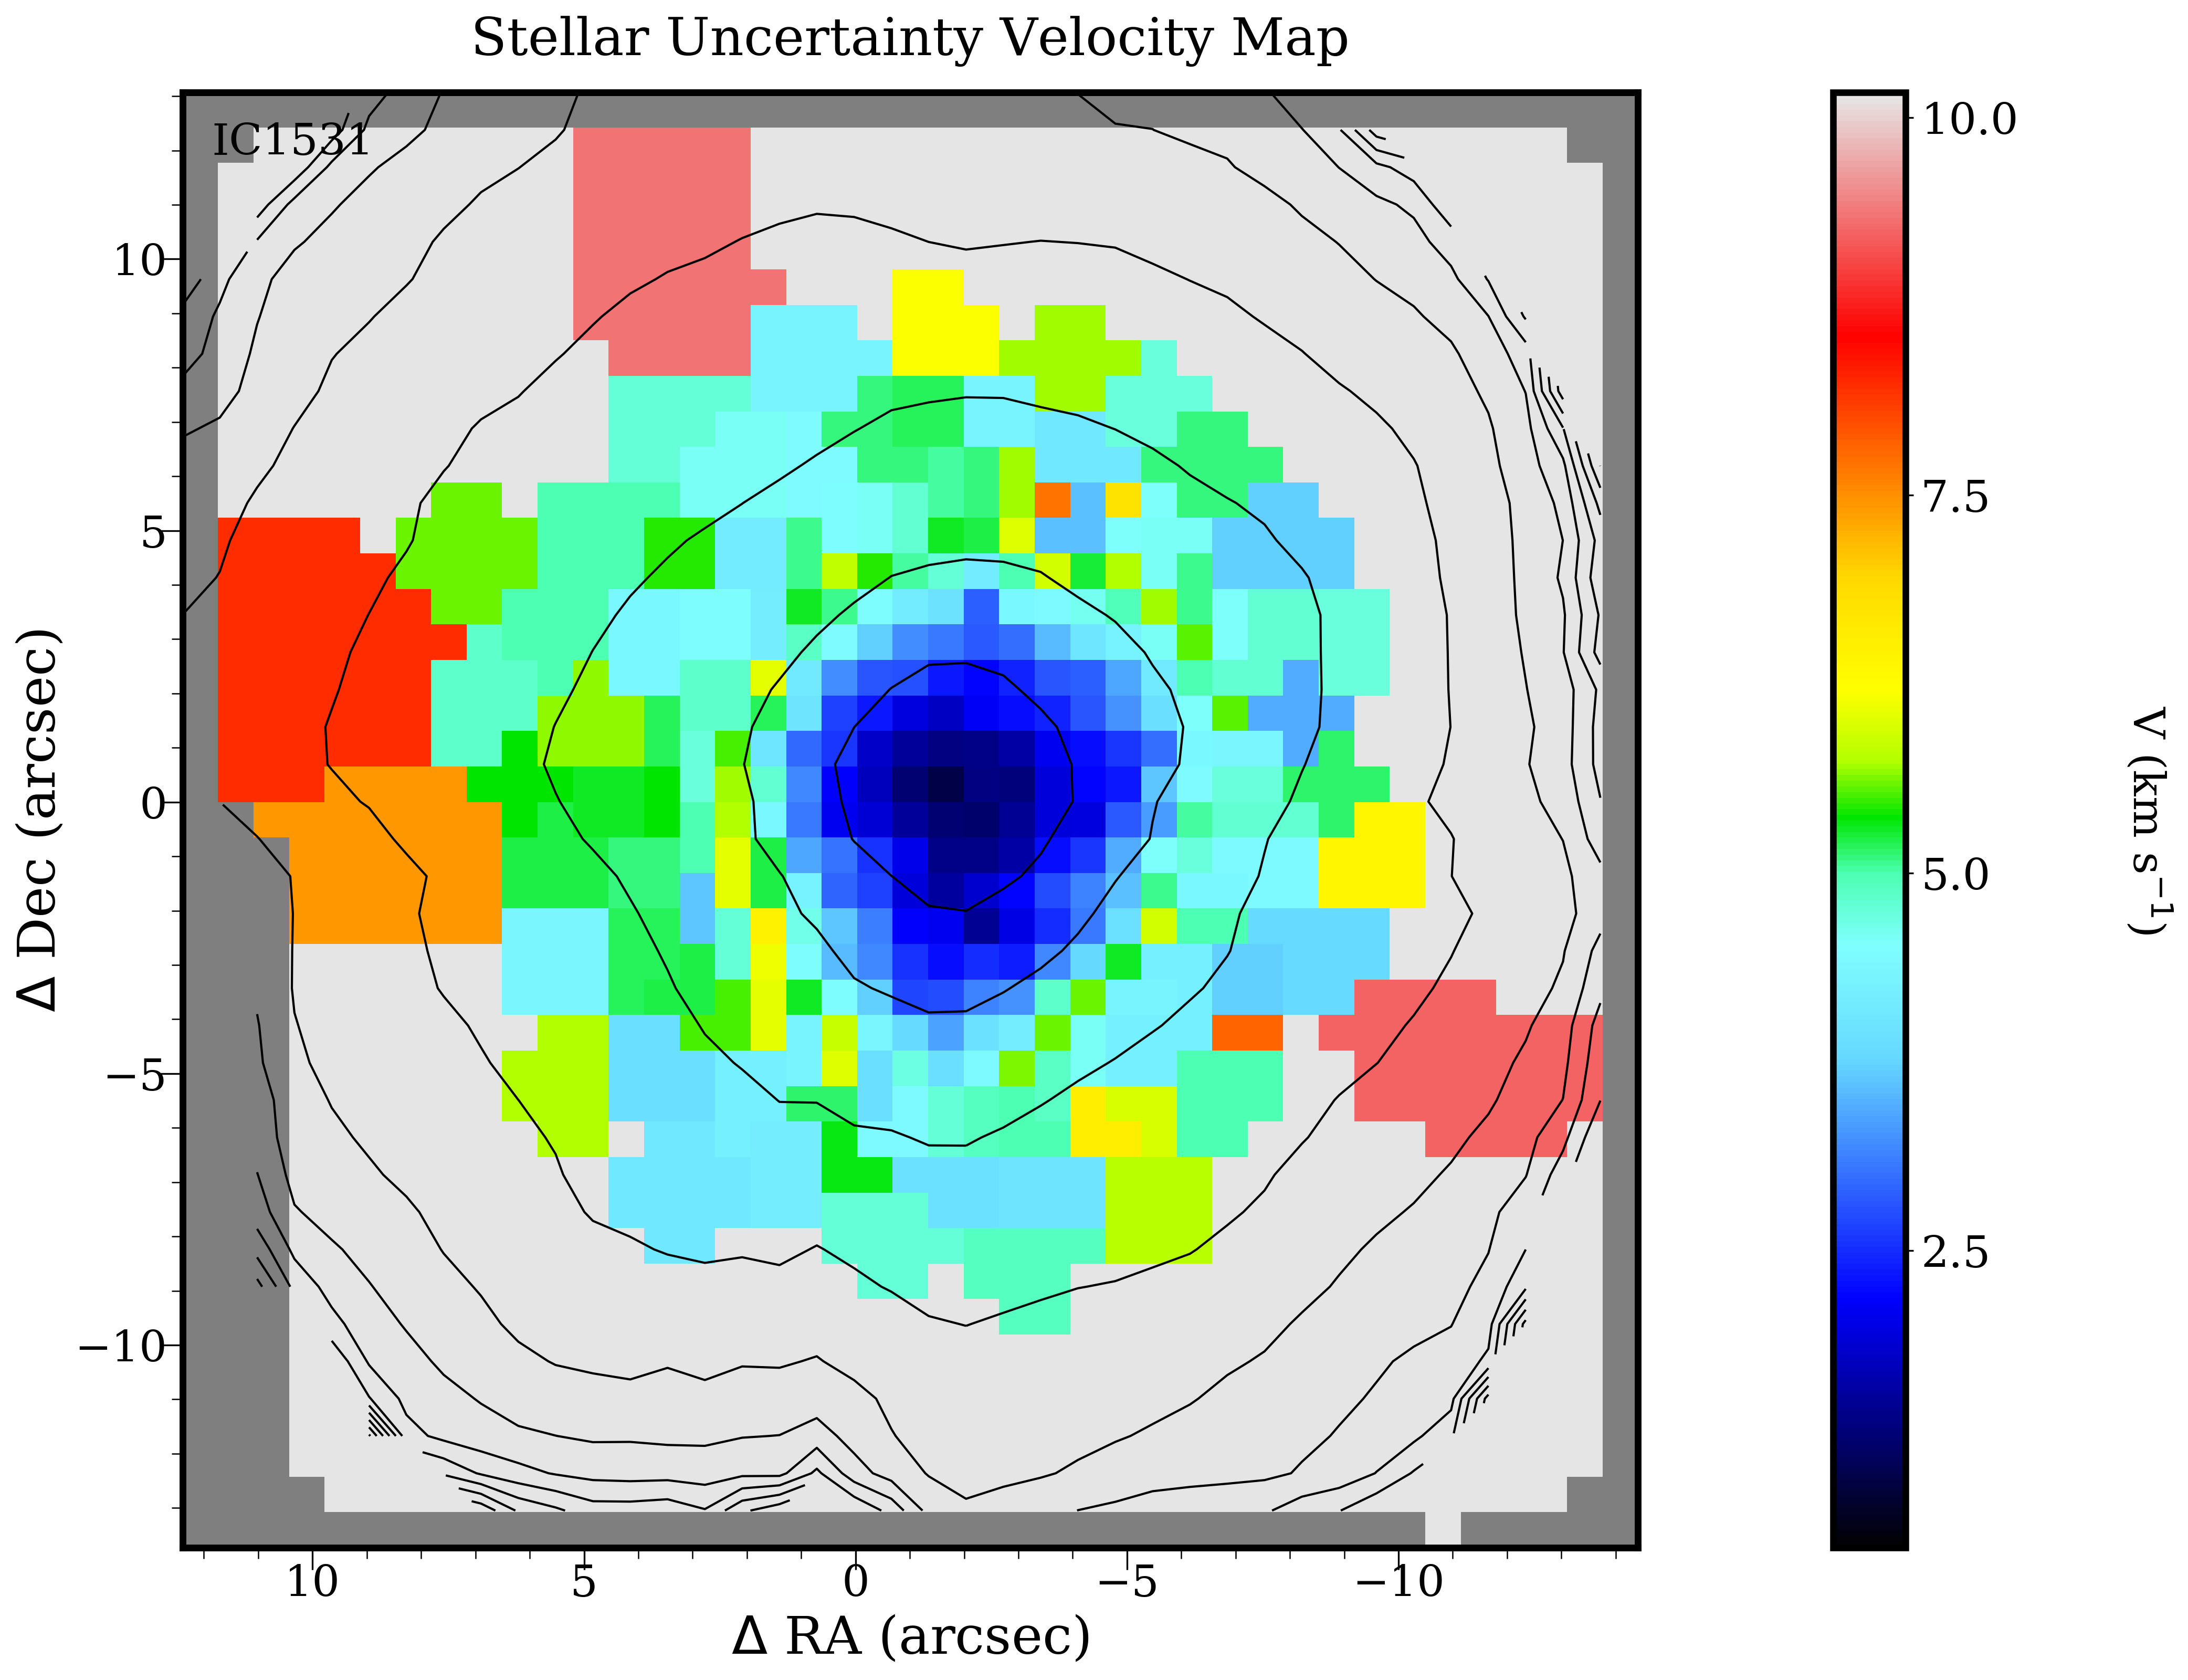
\includegraphics[width=0.245\textwidth]{Vmaps/ic1531_stellar_vel_uncert.png}
      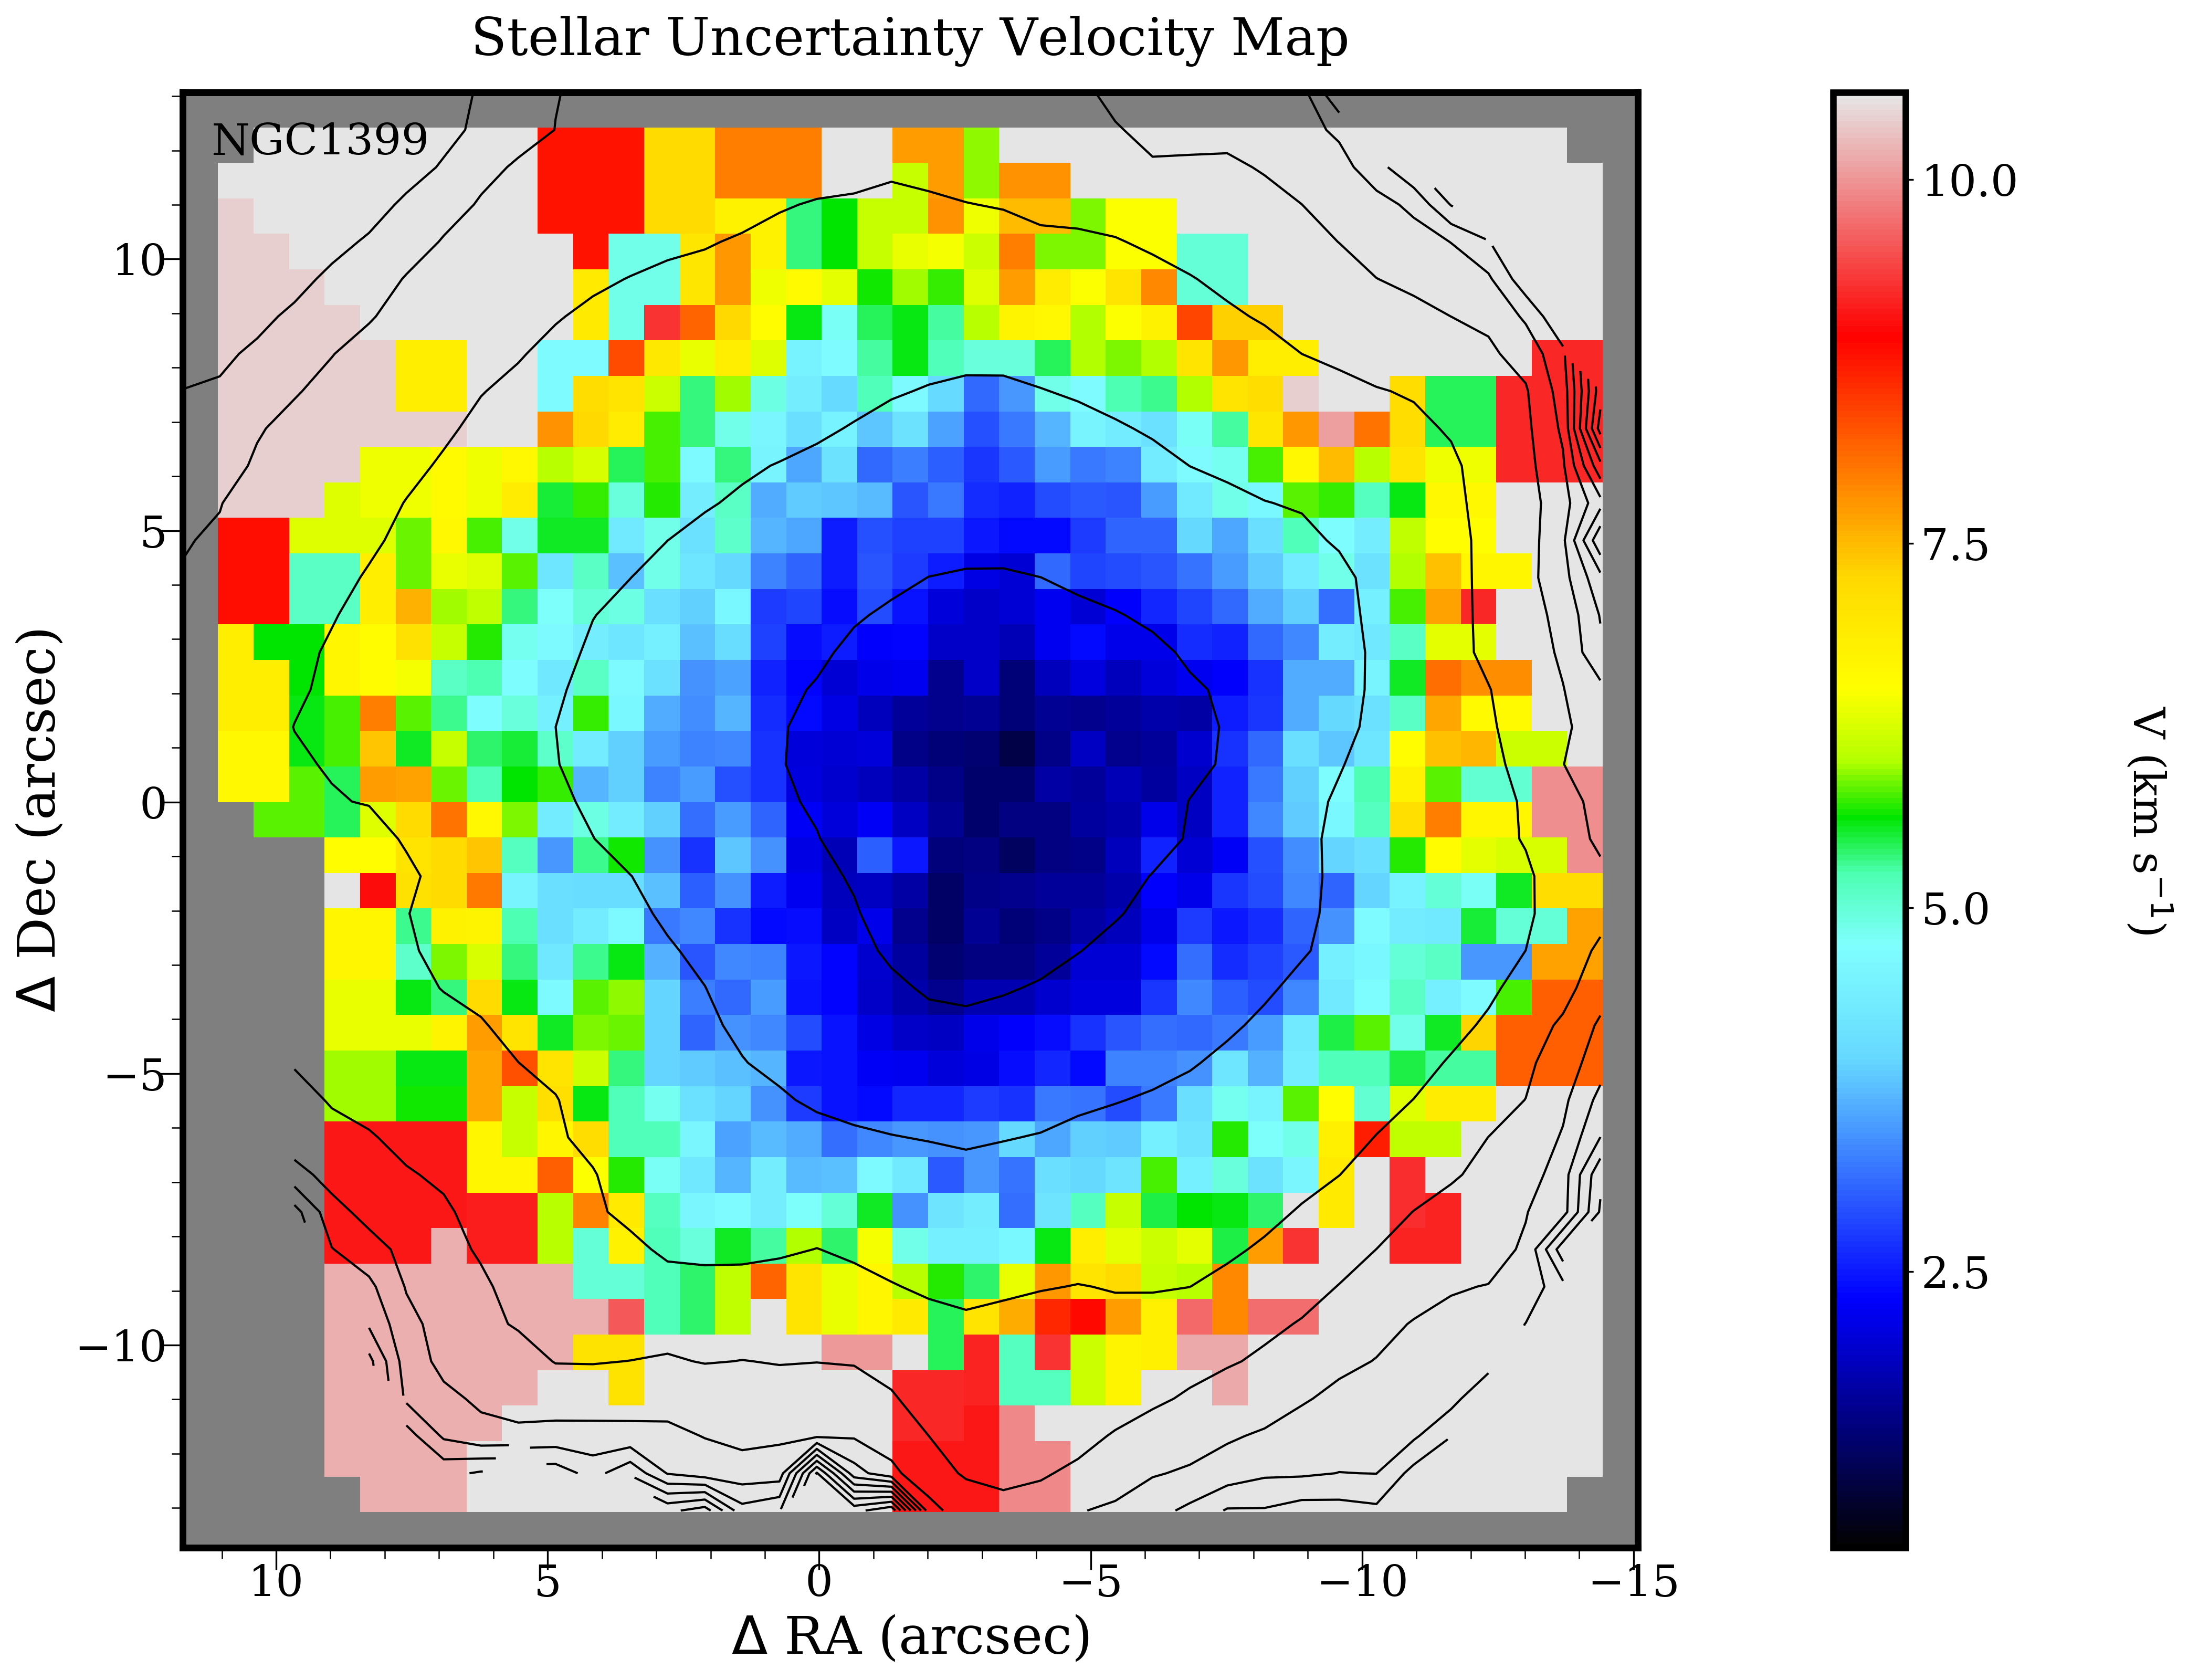
\includegraphics[width=0.245\textwidth]{Vmaps/ngc1399_stellar_vel_uncert.png}
      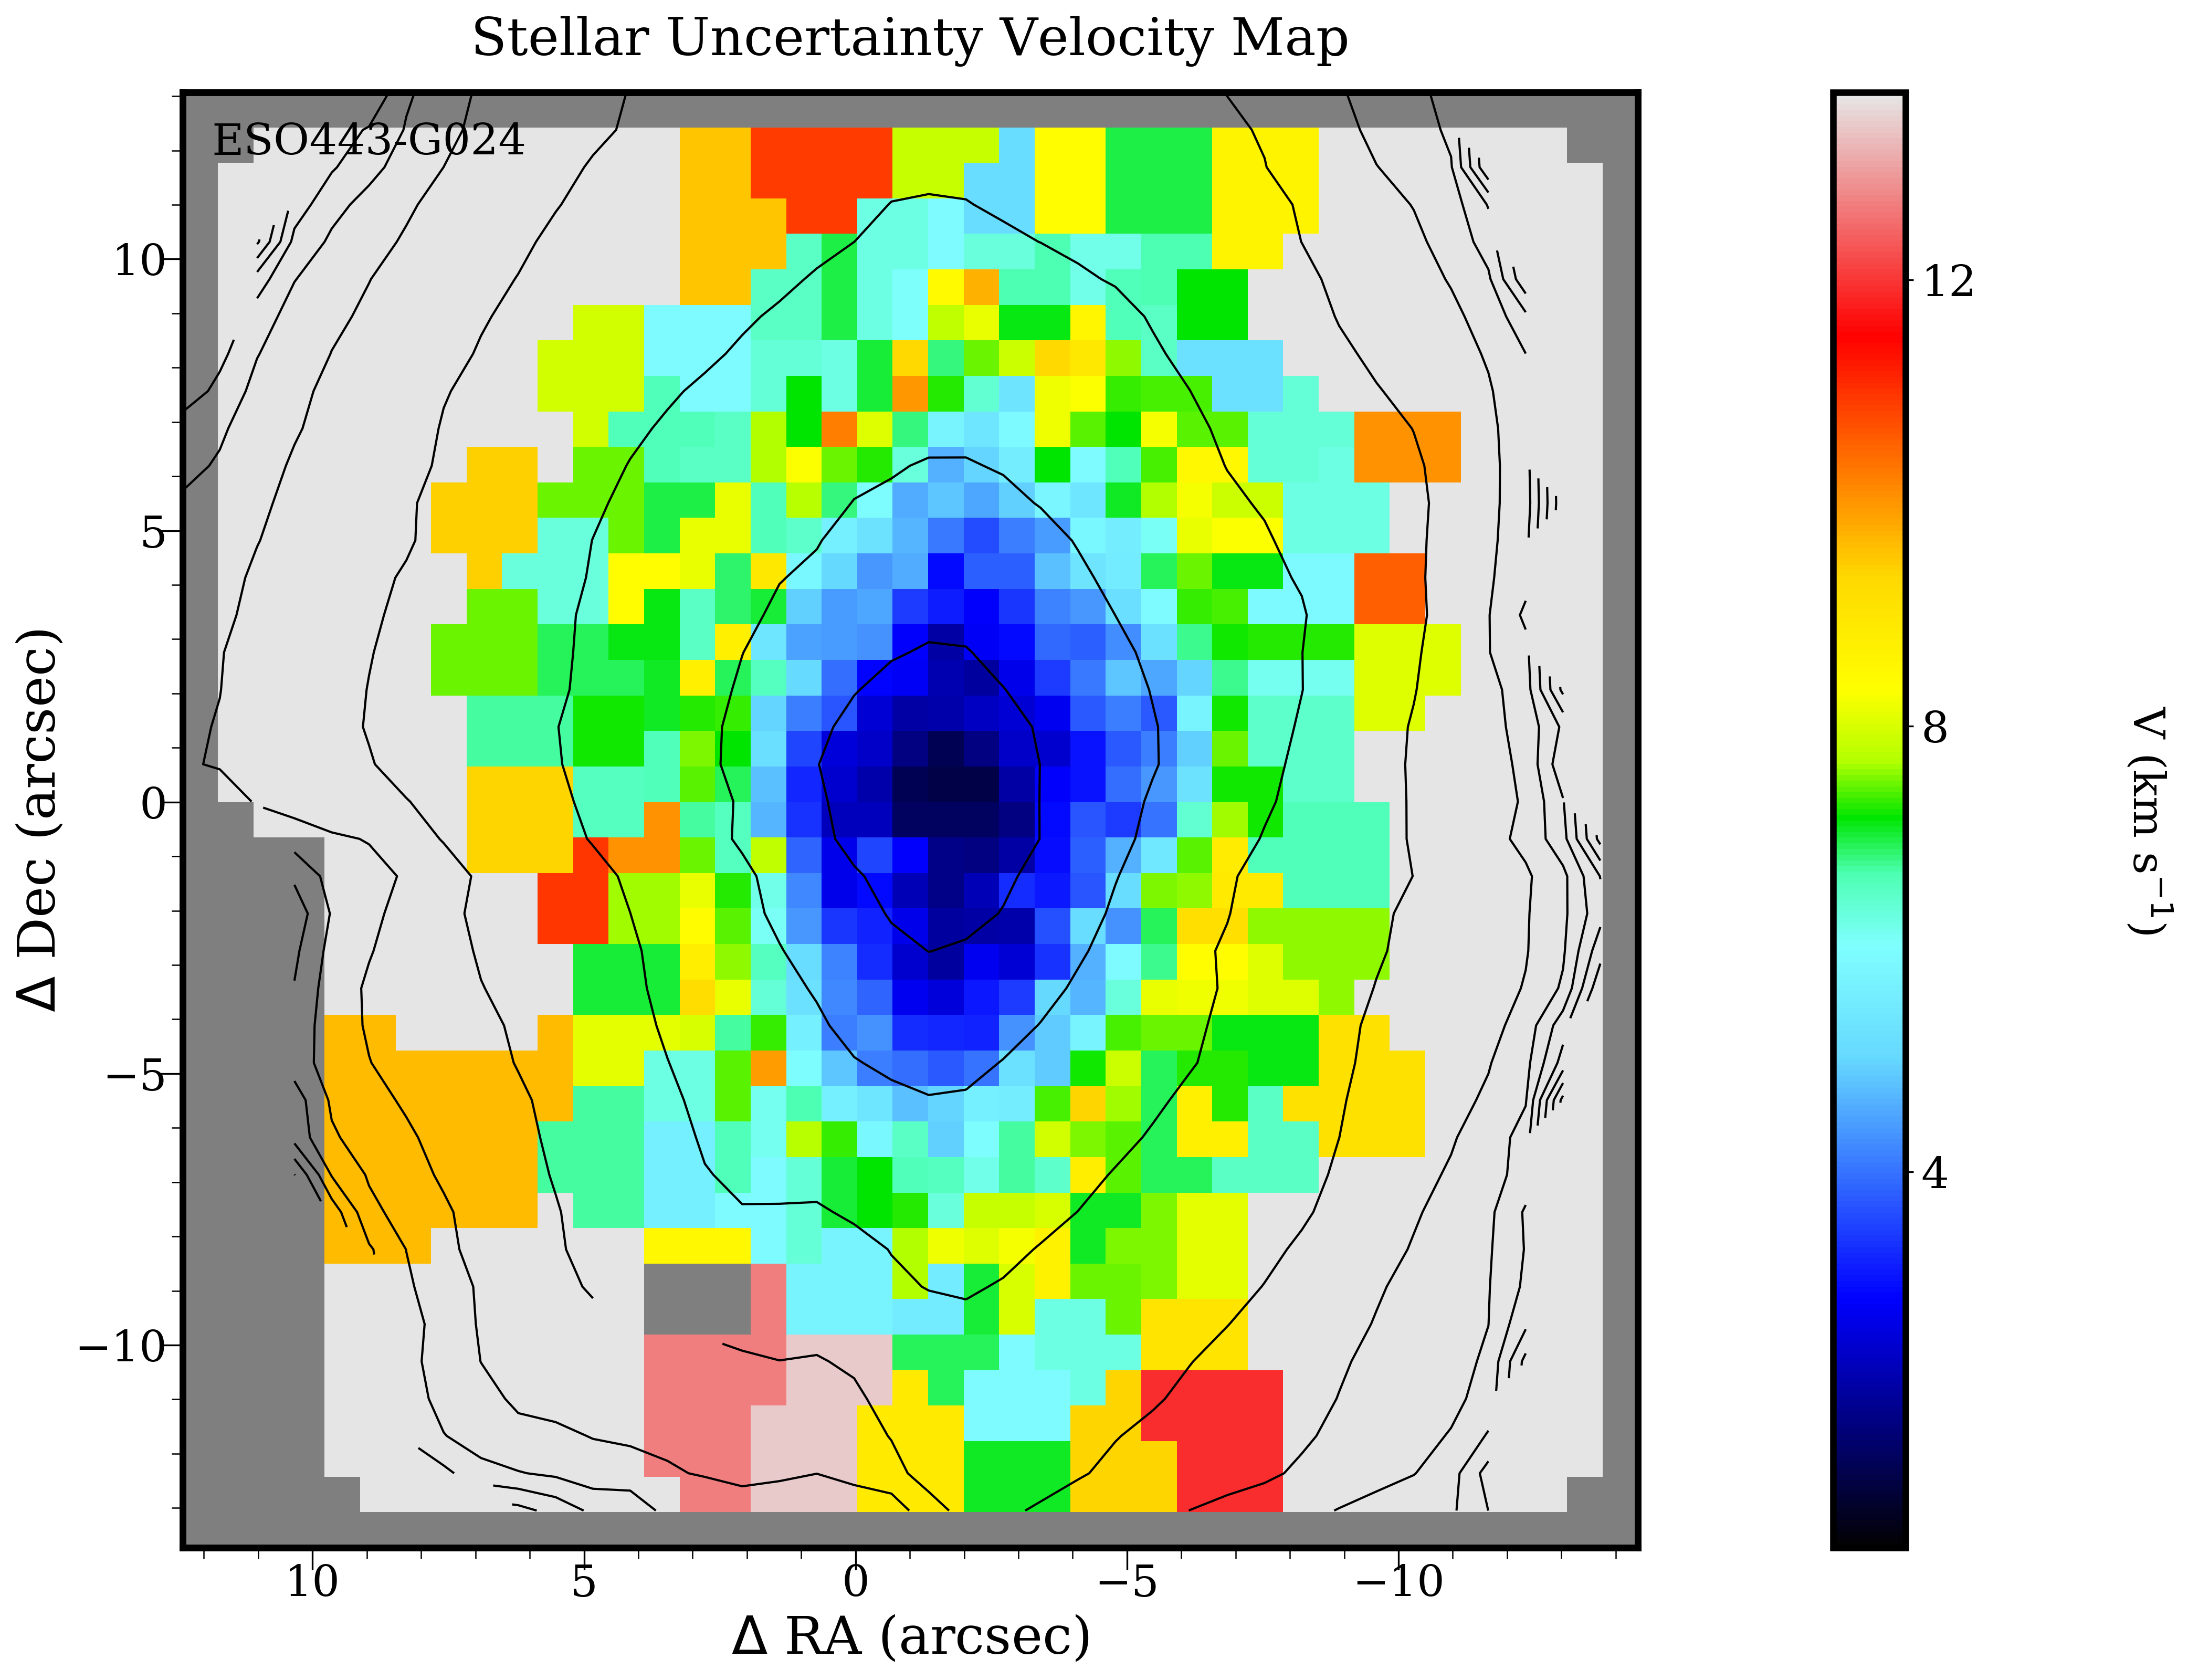
\includegraphics[width=0.245\textwidth]{Vmaps/eso443-g024_stellar_vel_uncert.png}
      \caption[VIMOS velocity uncertocity maps]{Uncertainties in the velocity for each galaxy in the VIMOS sample. Plots are ordered and contour colors are as in figure \ref{fig:Vstellar_img}}
      \label{fig:Vstellar_vel_uncert}
\end{figure*}

\begin{figure*}
      \centering
      \includegraphics[width=0.245\textwidth]{Vmaps/ngc0612_stellar_sigma.png}
      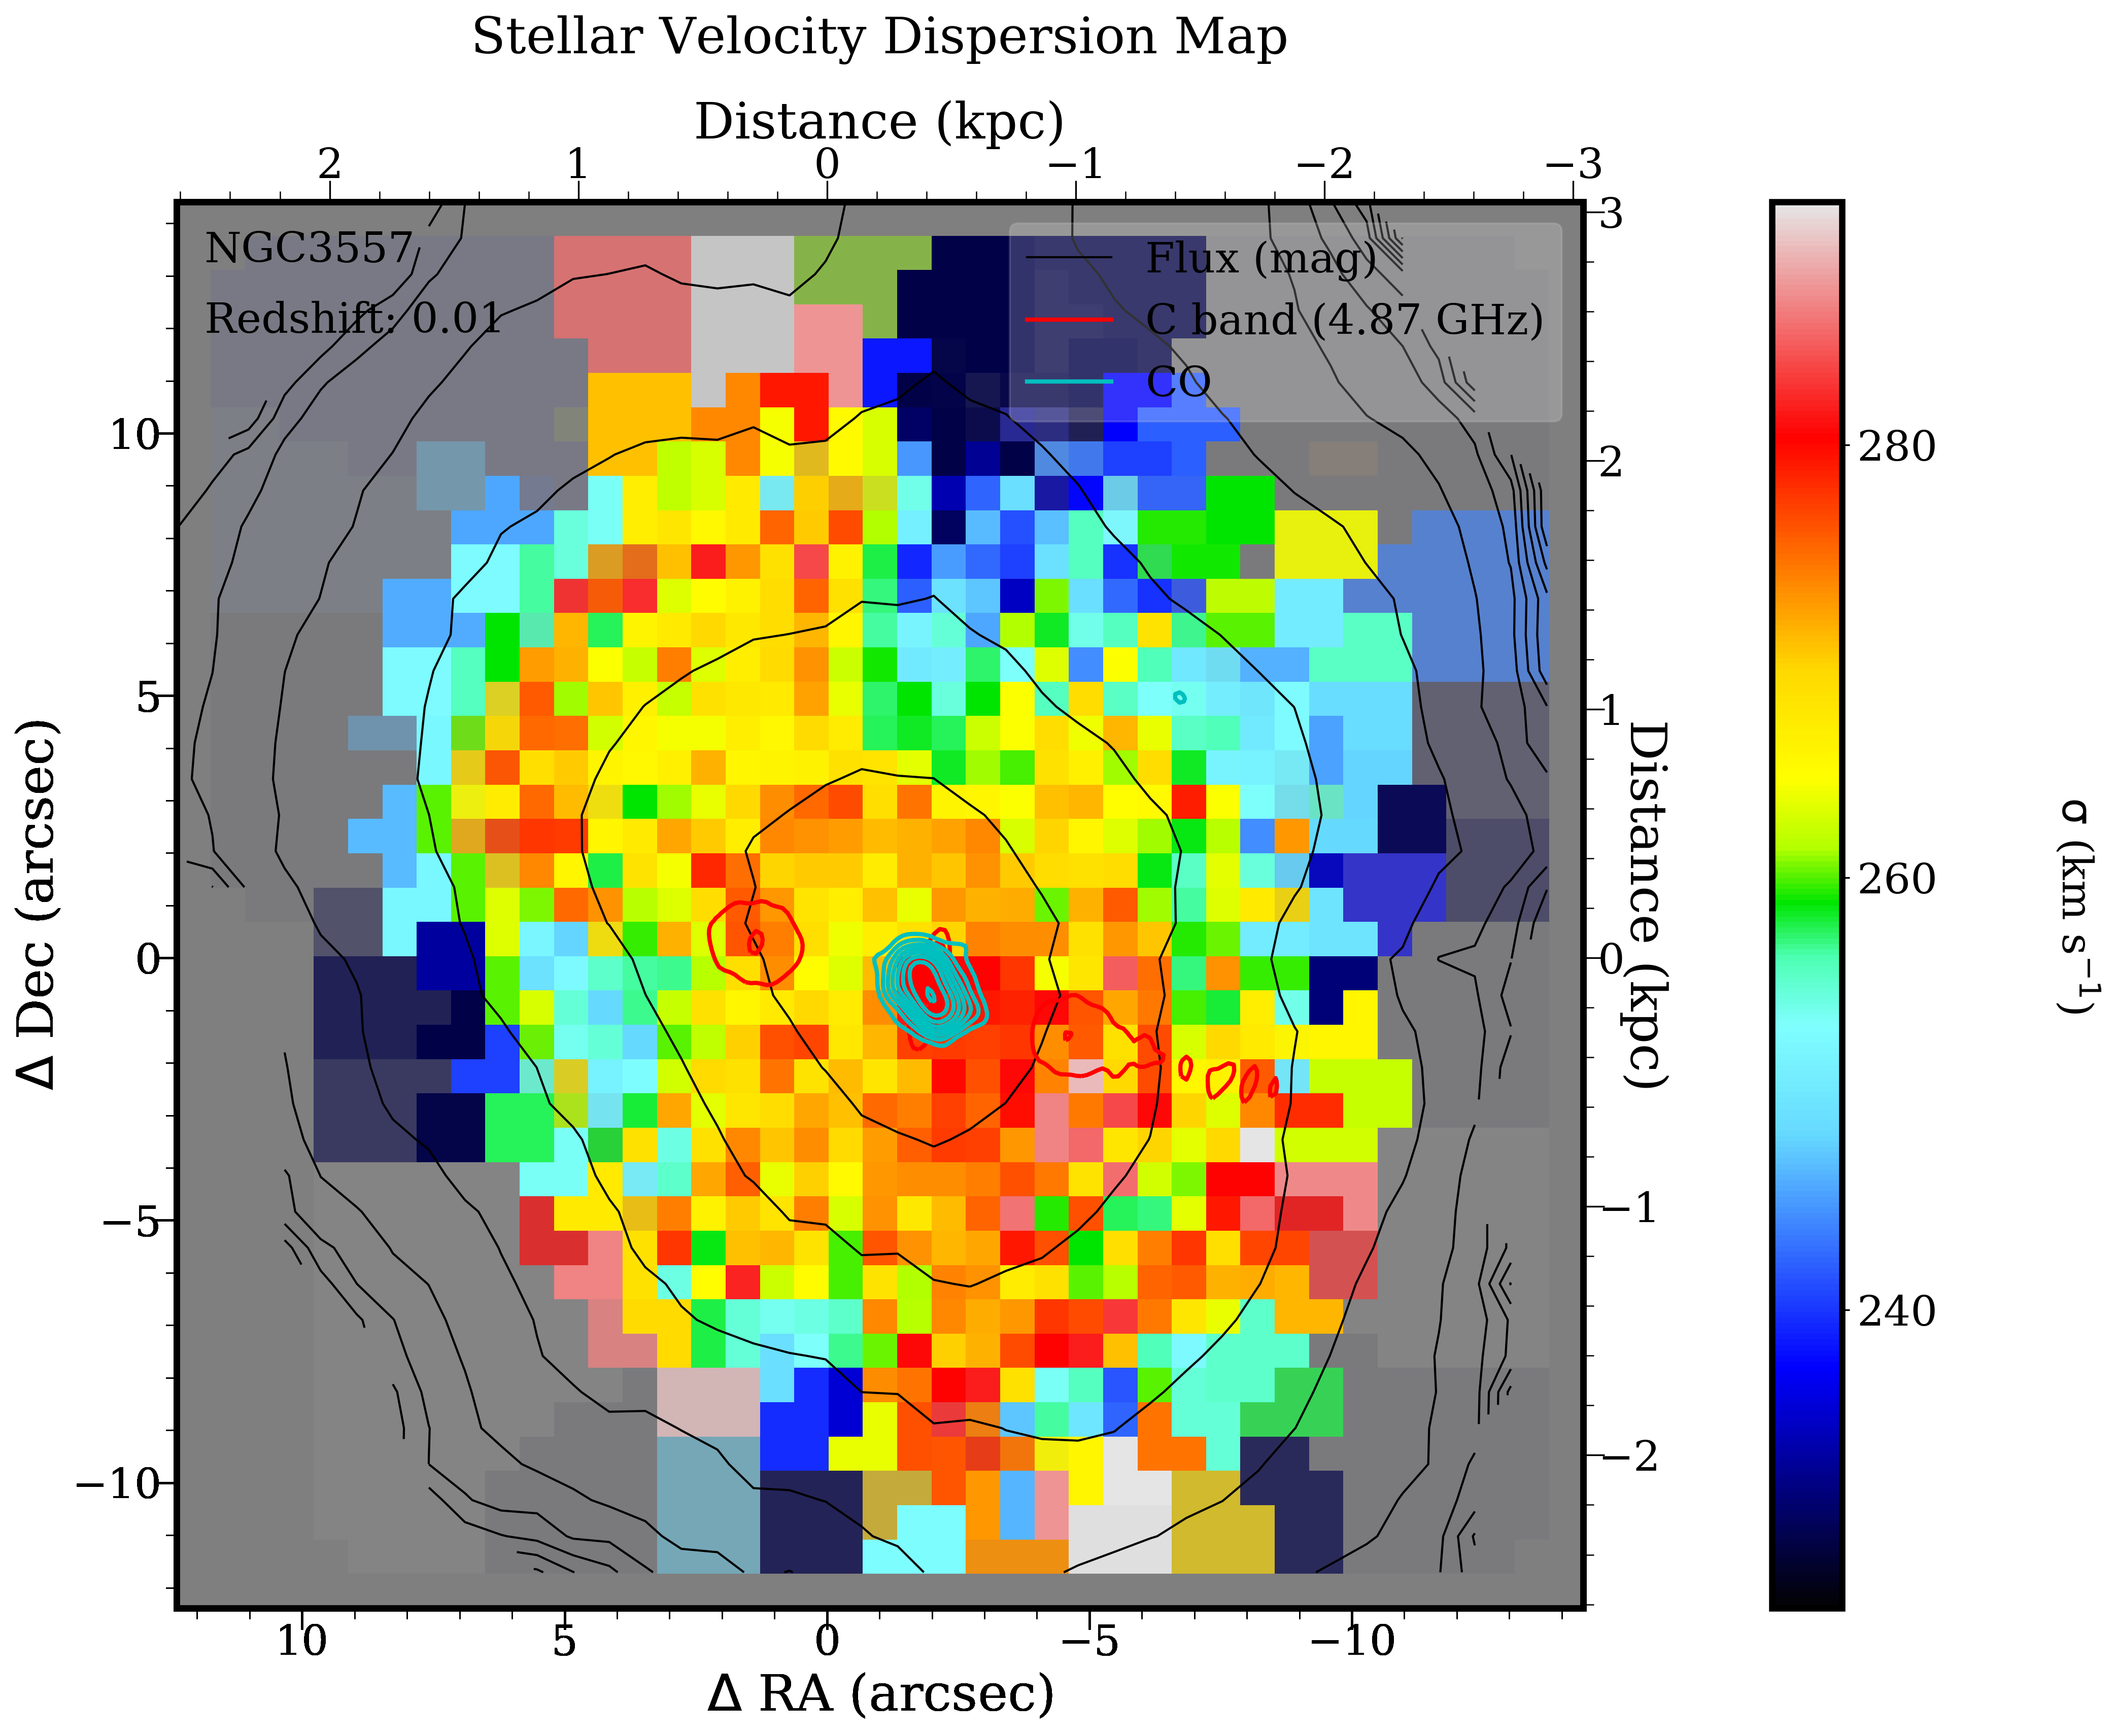
\includegraphics[width=0.245\textwidth]{Vmaps/ngc3557_stellar_sigma.png}
      \includegraphics[width=0.245\textwidth]{Vmaps/ngc3100_stellar_sigma.png}
      \includegraphics[width=0.245\textwidth]{Vmaps/ic1459_stellar_sigma.png}
      \includegraphics[width=0.245\textwidth]{Vmaps/pks0718-34_stellar_sigma.png}
      \includegraphics[width=0.245\textwidth]{Vmaps/ic4296_stellar_sigma.png}
      \includegraphics[width=0.245\textwidth]{Vmaps/ngc7075_stellar_sigma.png}
      \includegraphics[width=0.245\textwidth]{Vmaps/ic1531_stellar_sigma.png}
      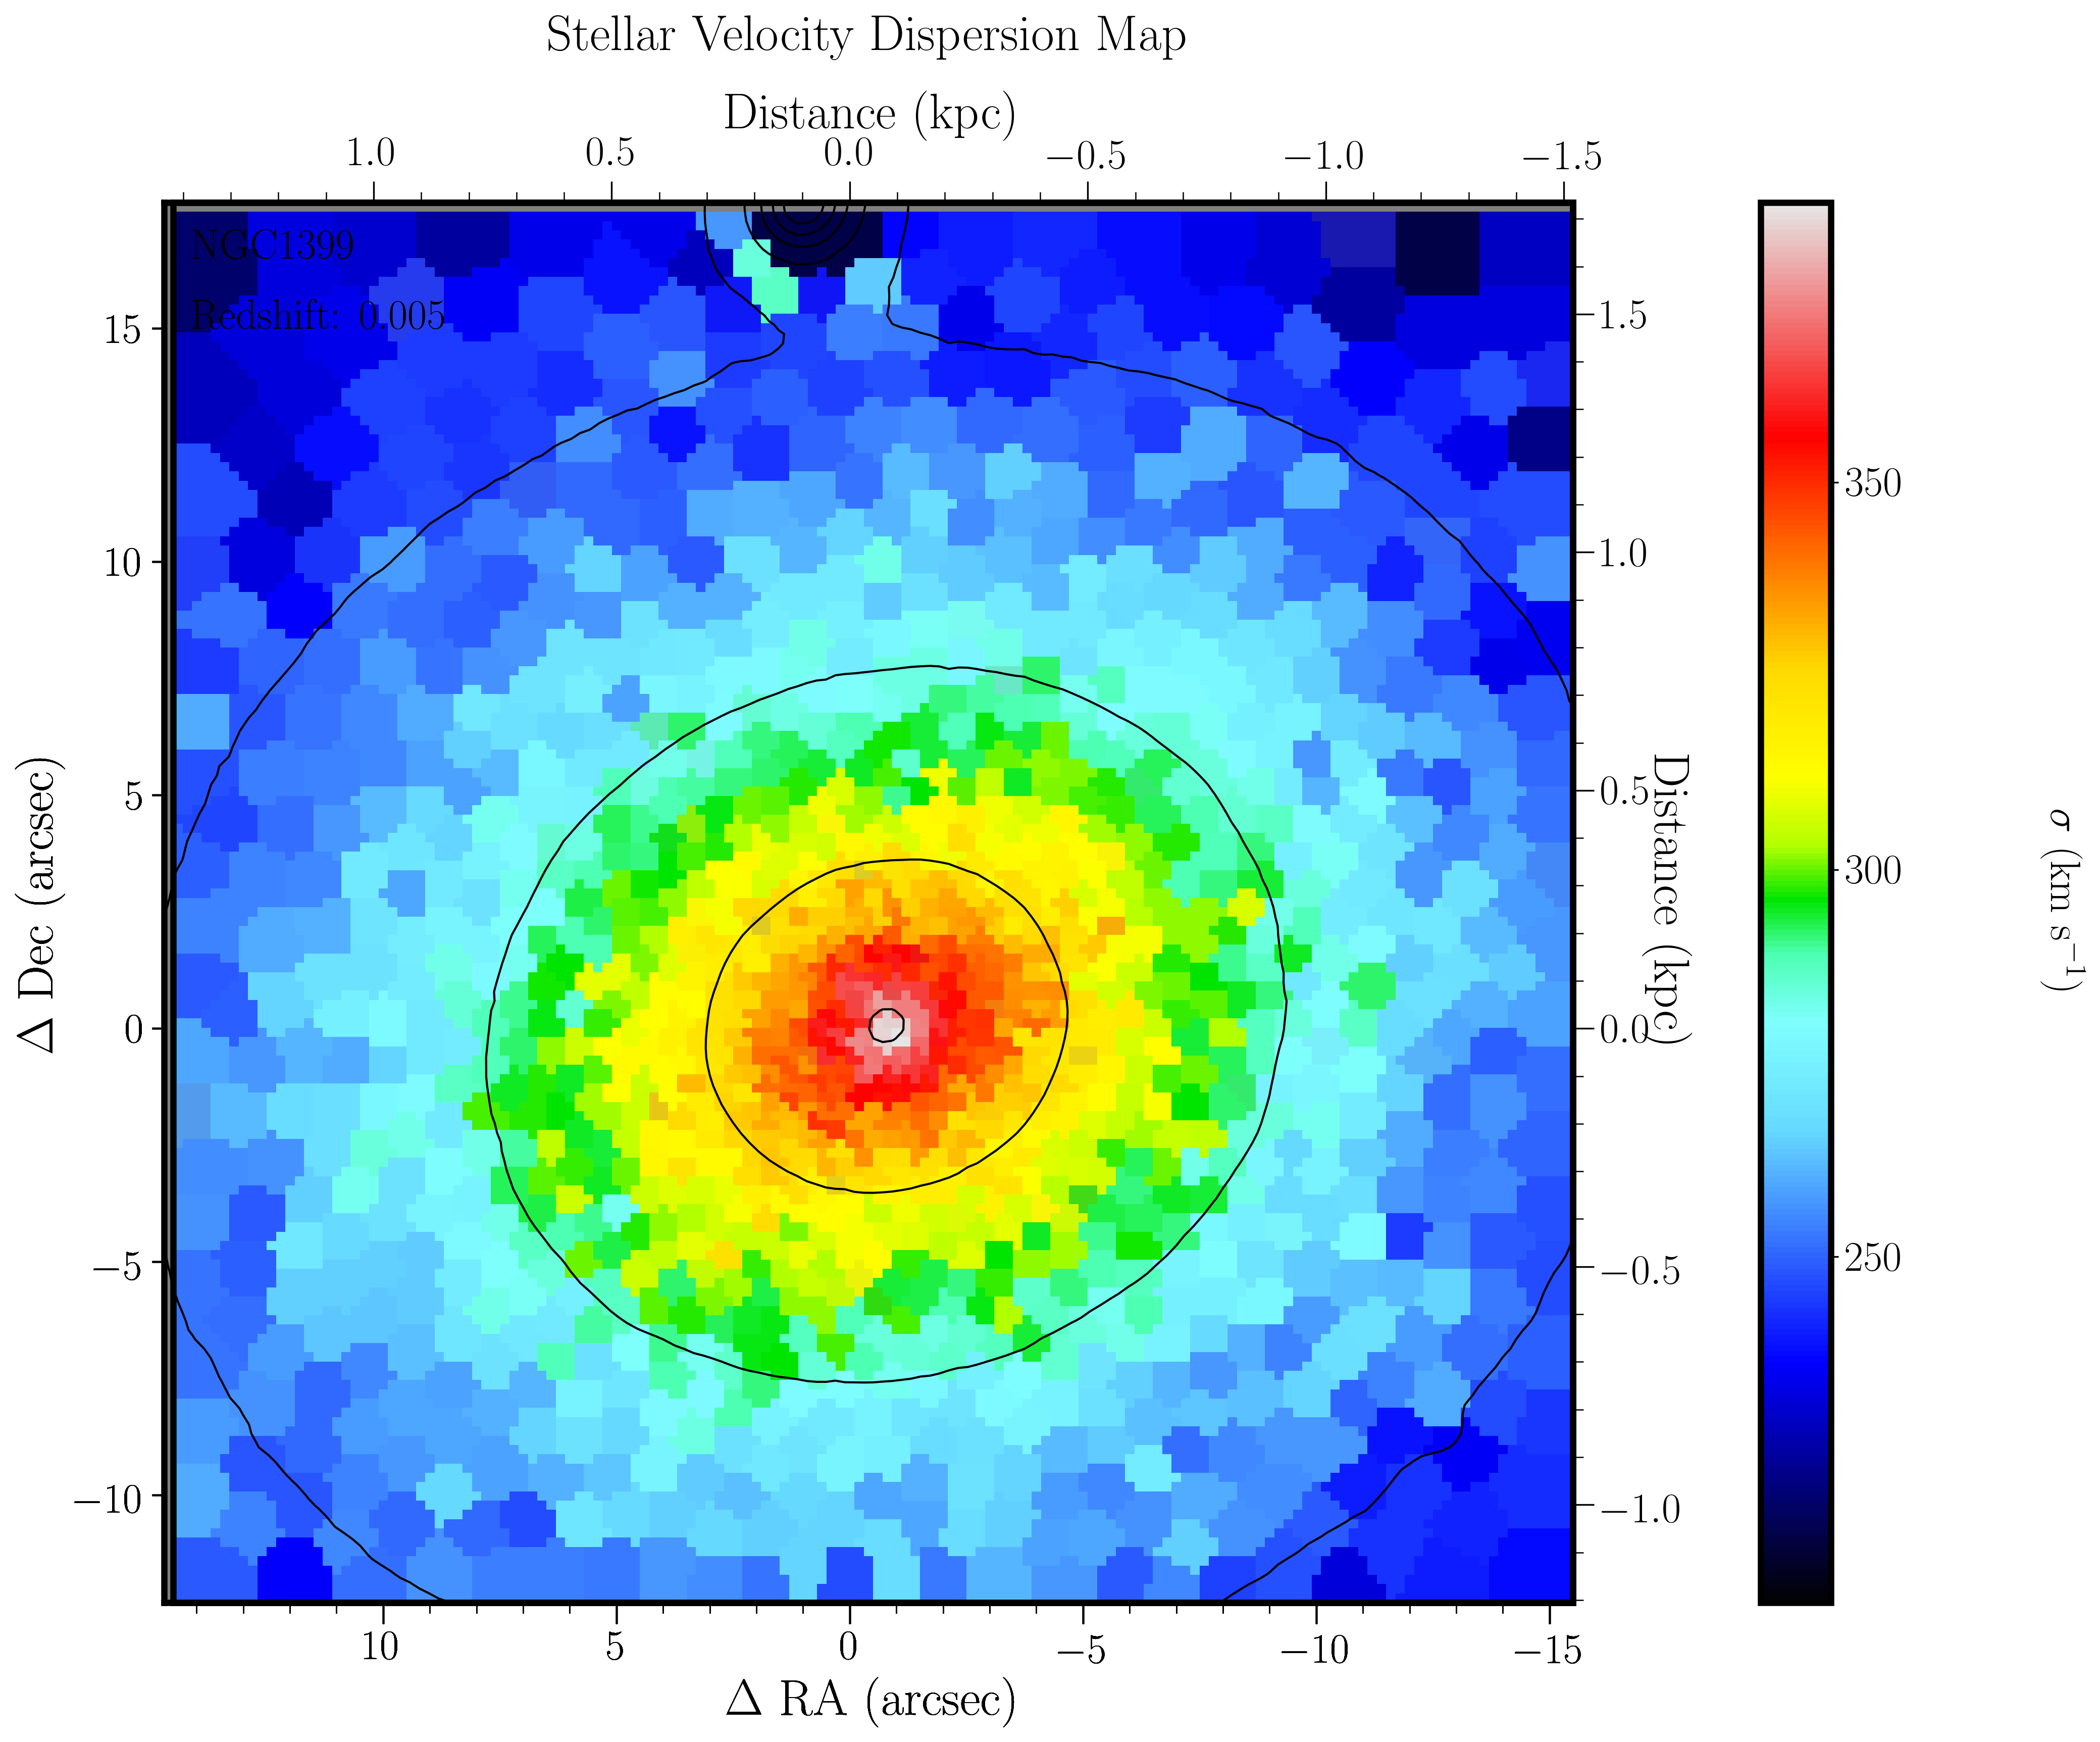
\includegraphics[width=0.245\textwidth]{Vmaps/ngc1399_stellar_sigma.png}
      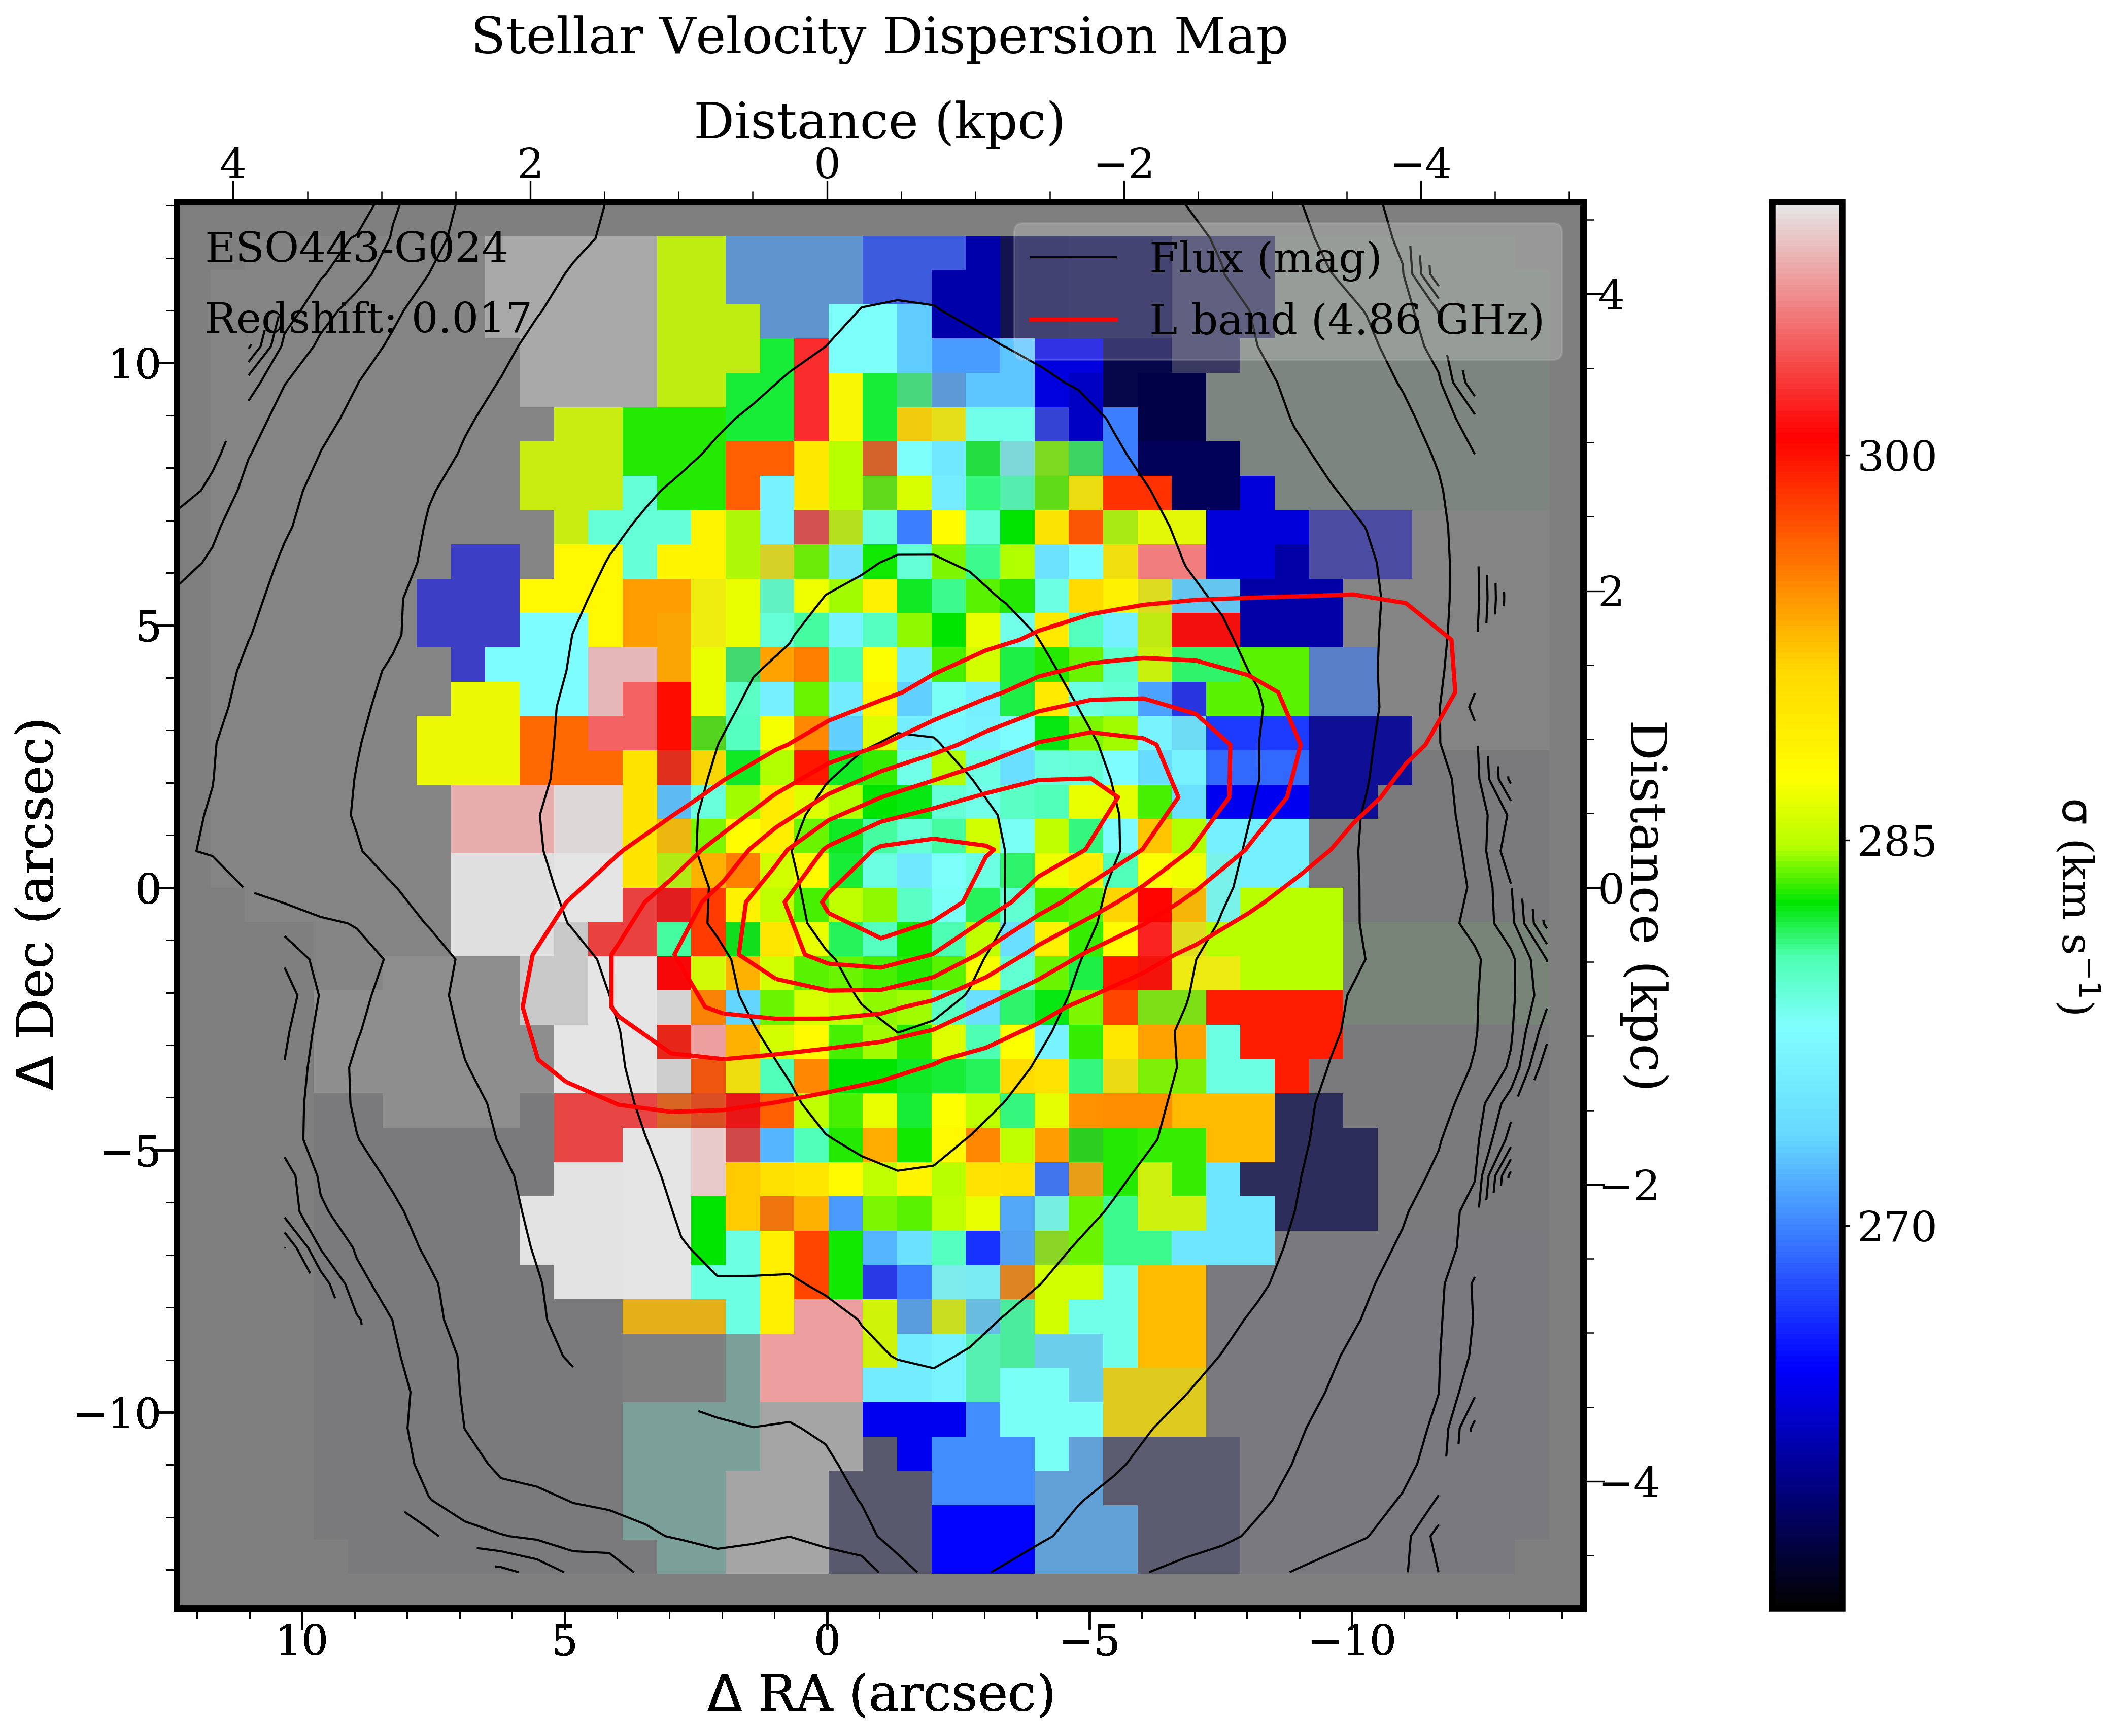
\includegraphics[width=0.245\textwidth]{Vmaps/eso443-g024_stellar_sigma.png}
      \caption[VIMOS velocity dispersion]{Velocity dispersion for each galaxy in the VIMOS sample. Plots are ordered and contour colors are as in figure \ref{fig:Vstellar_img}}
      \label{fig:Vstellar_sigma}
\end{figure*}


\begin{figure*}
      \centering
      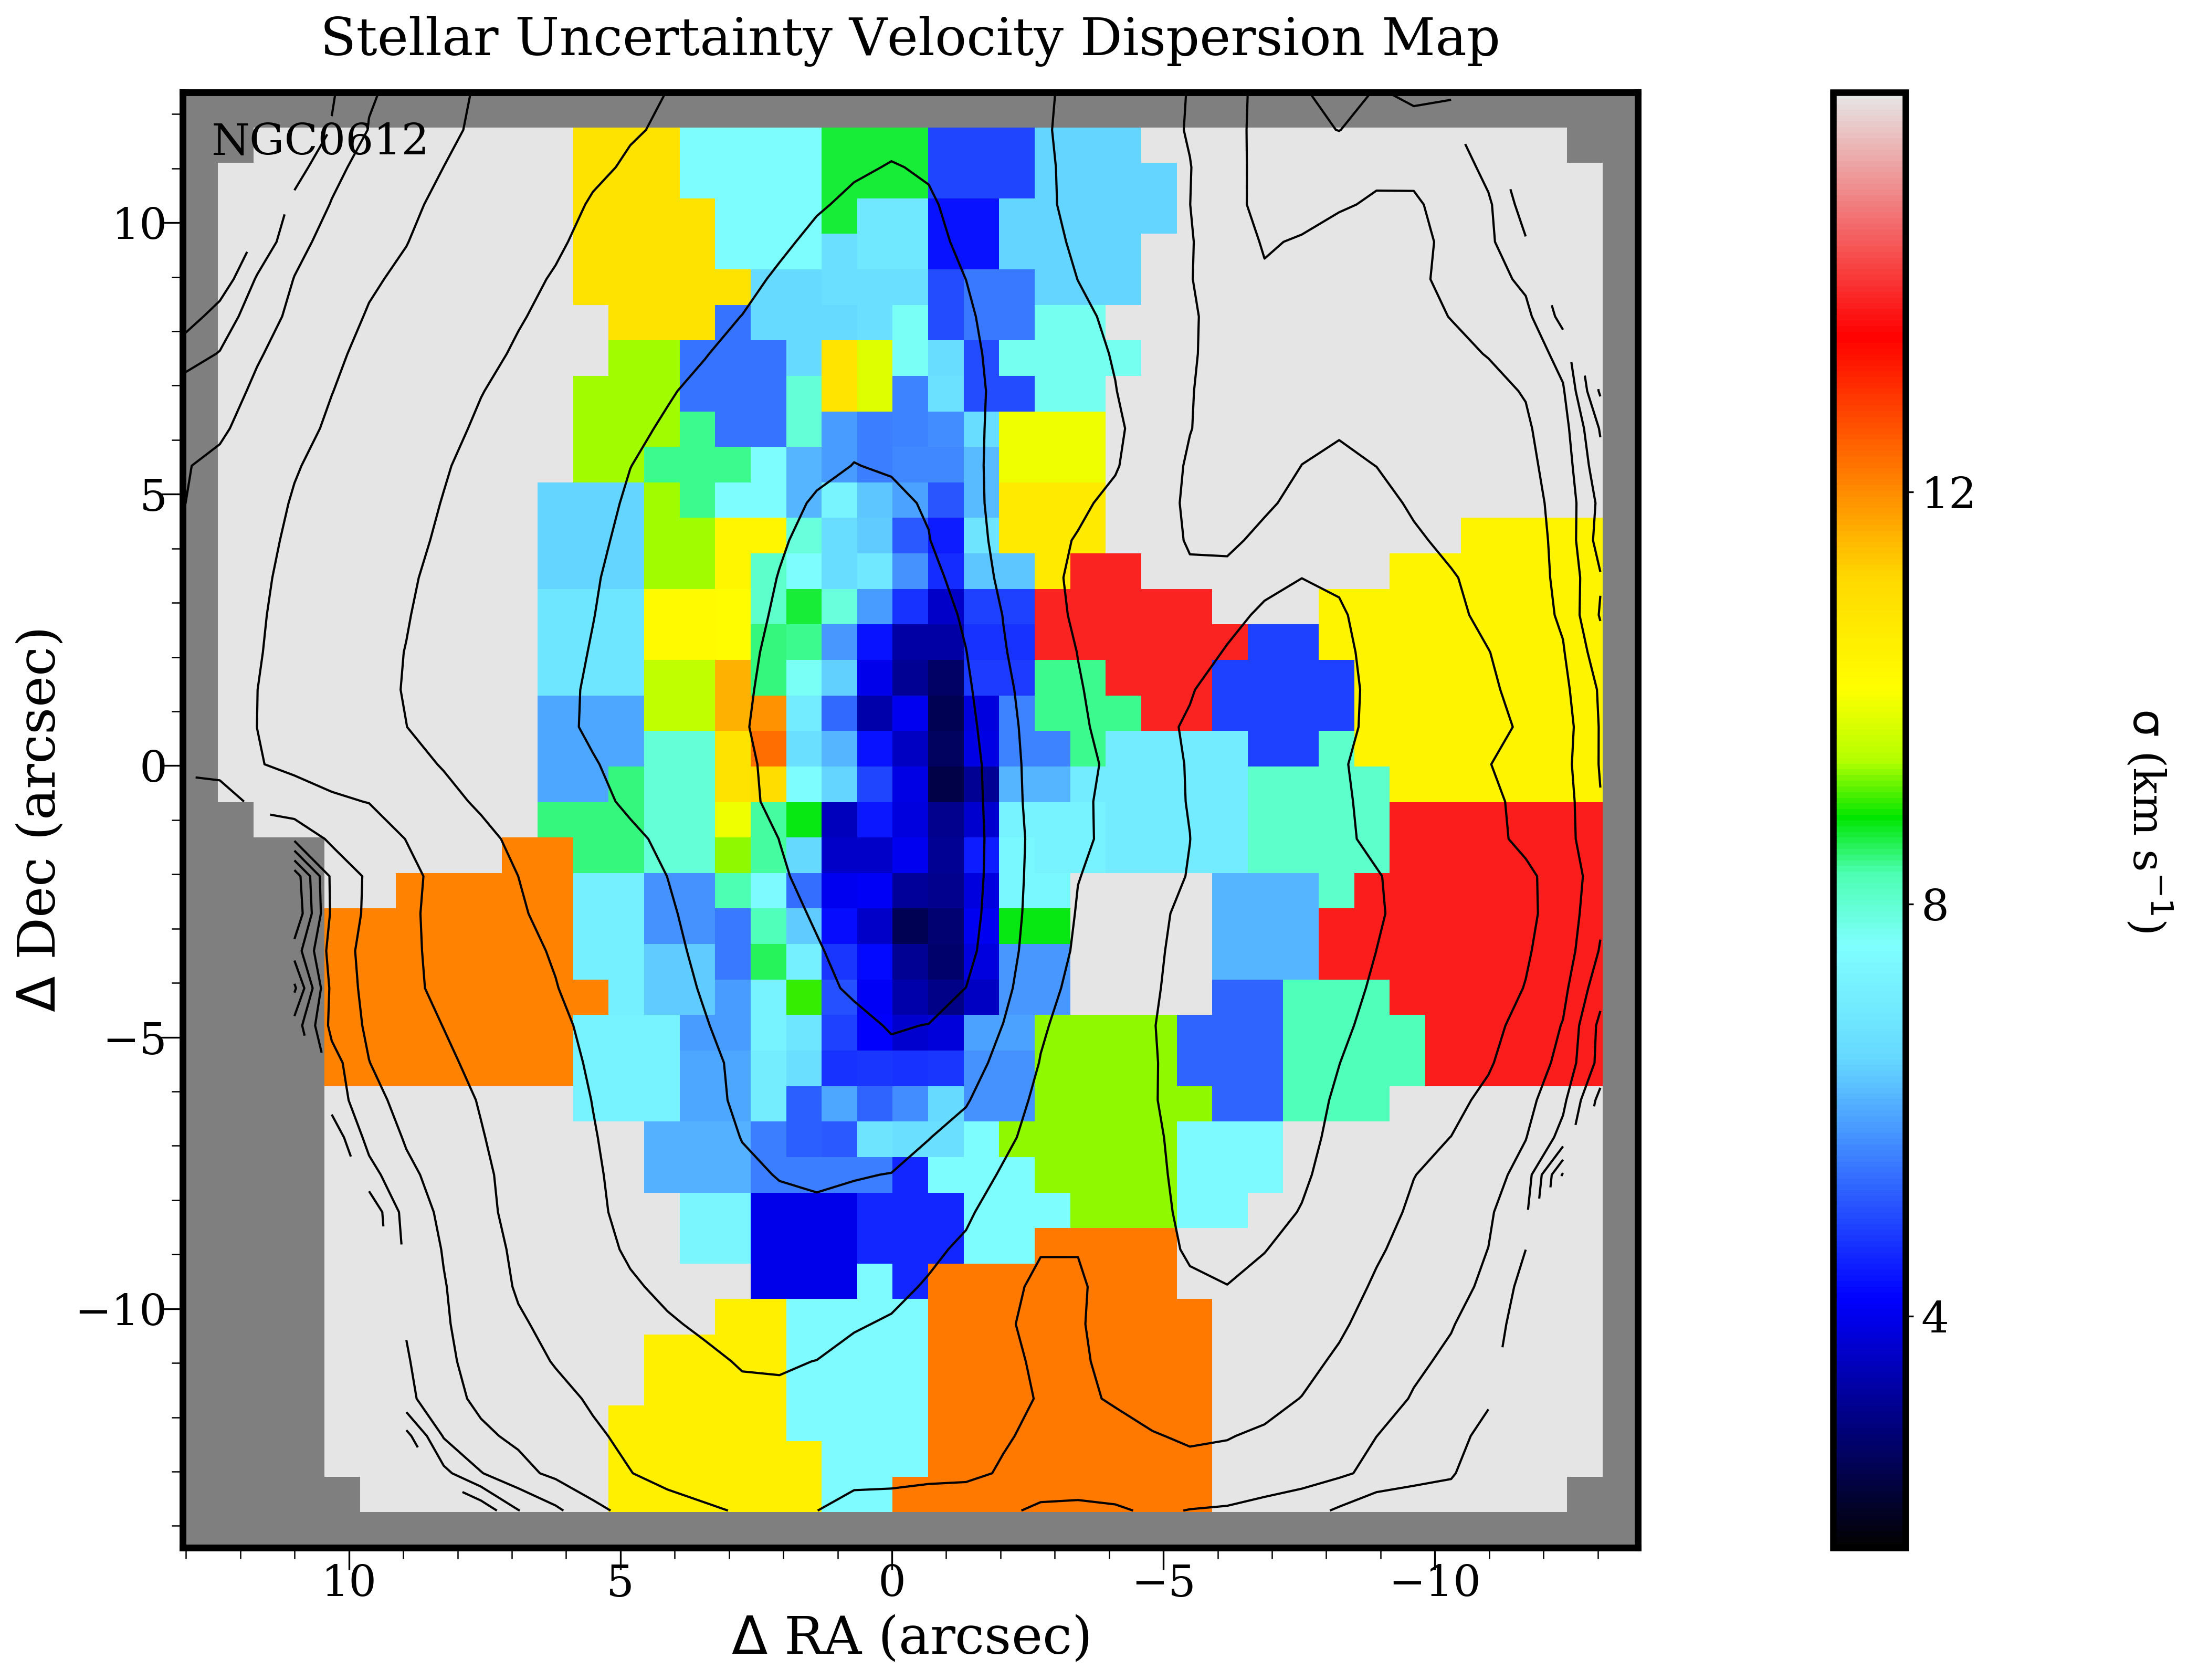
\includegraphics[width=0.245\textwidth]{Vmaps/ngc0612_stellar_sigma_uncert.png}
      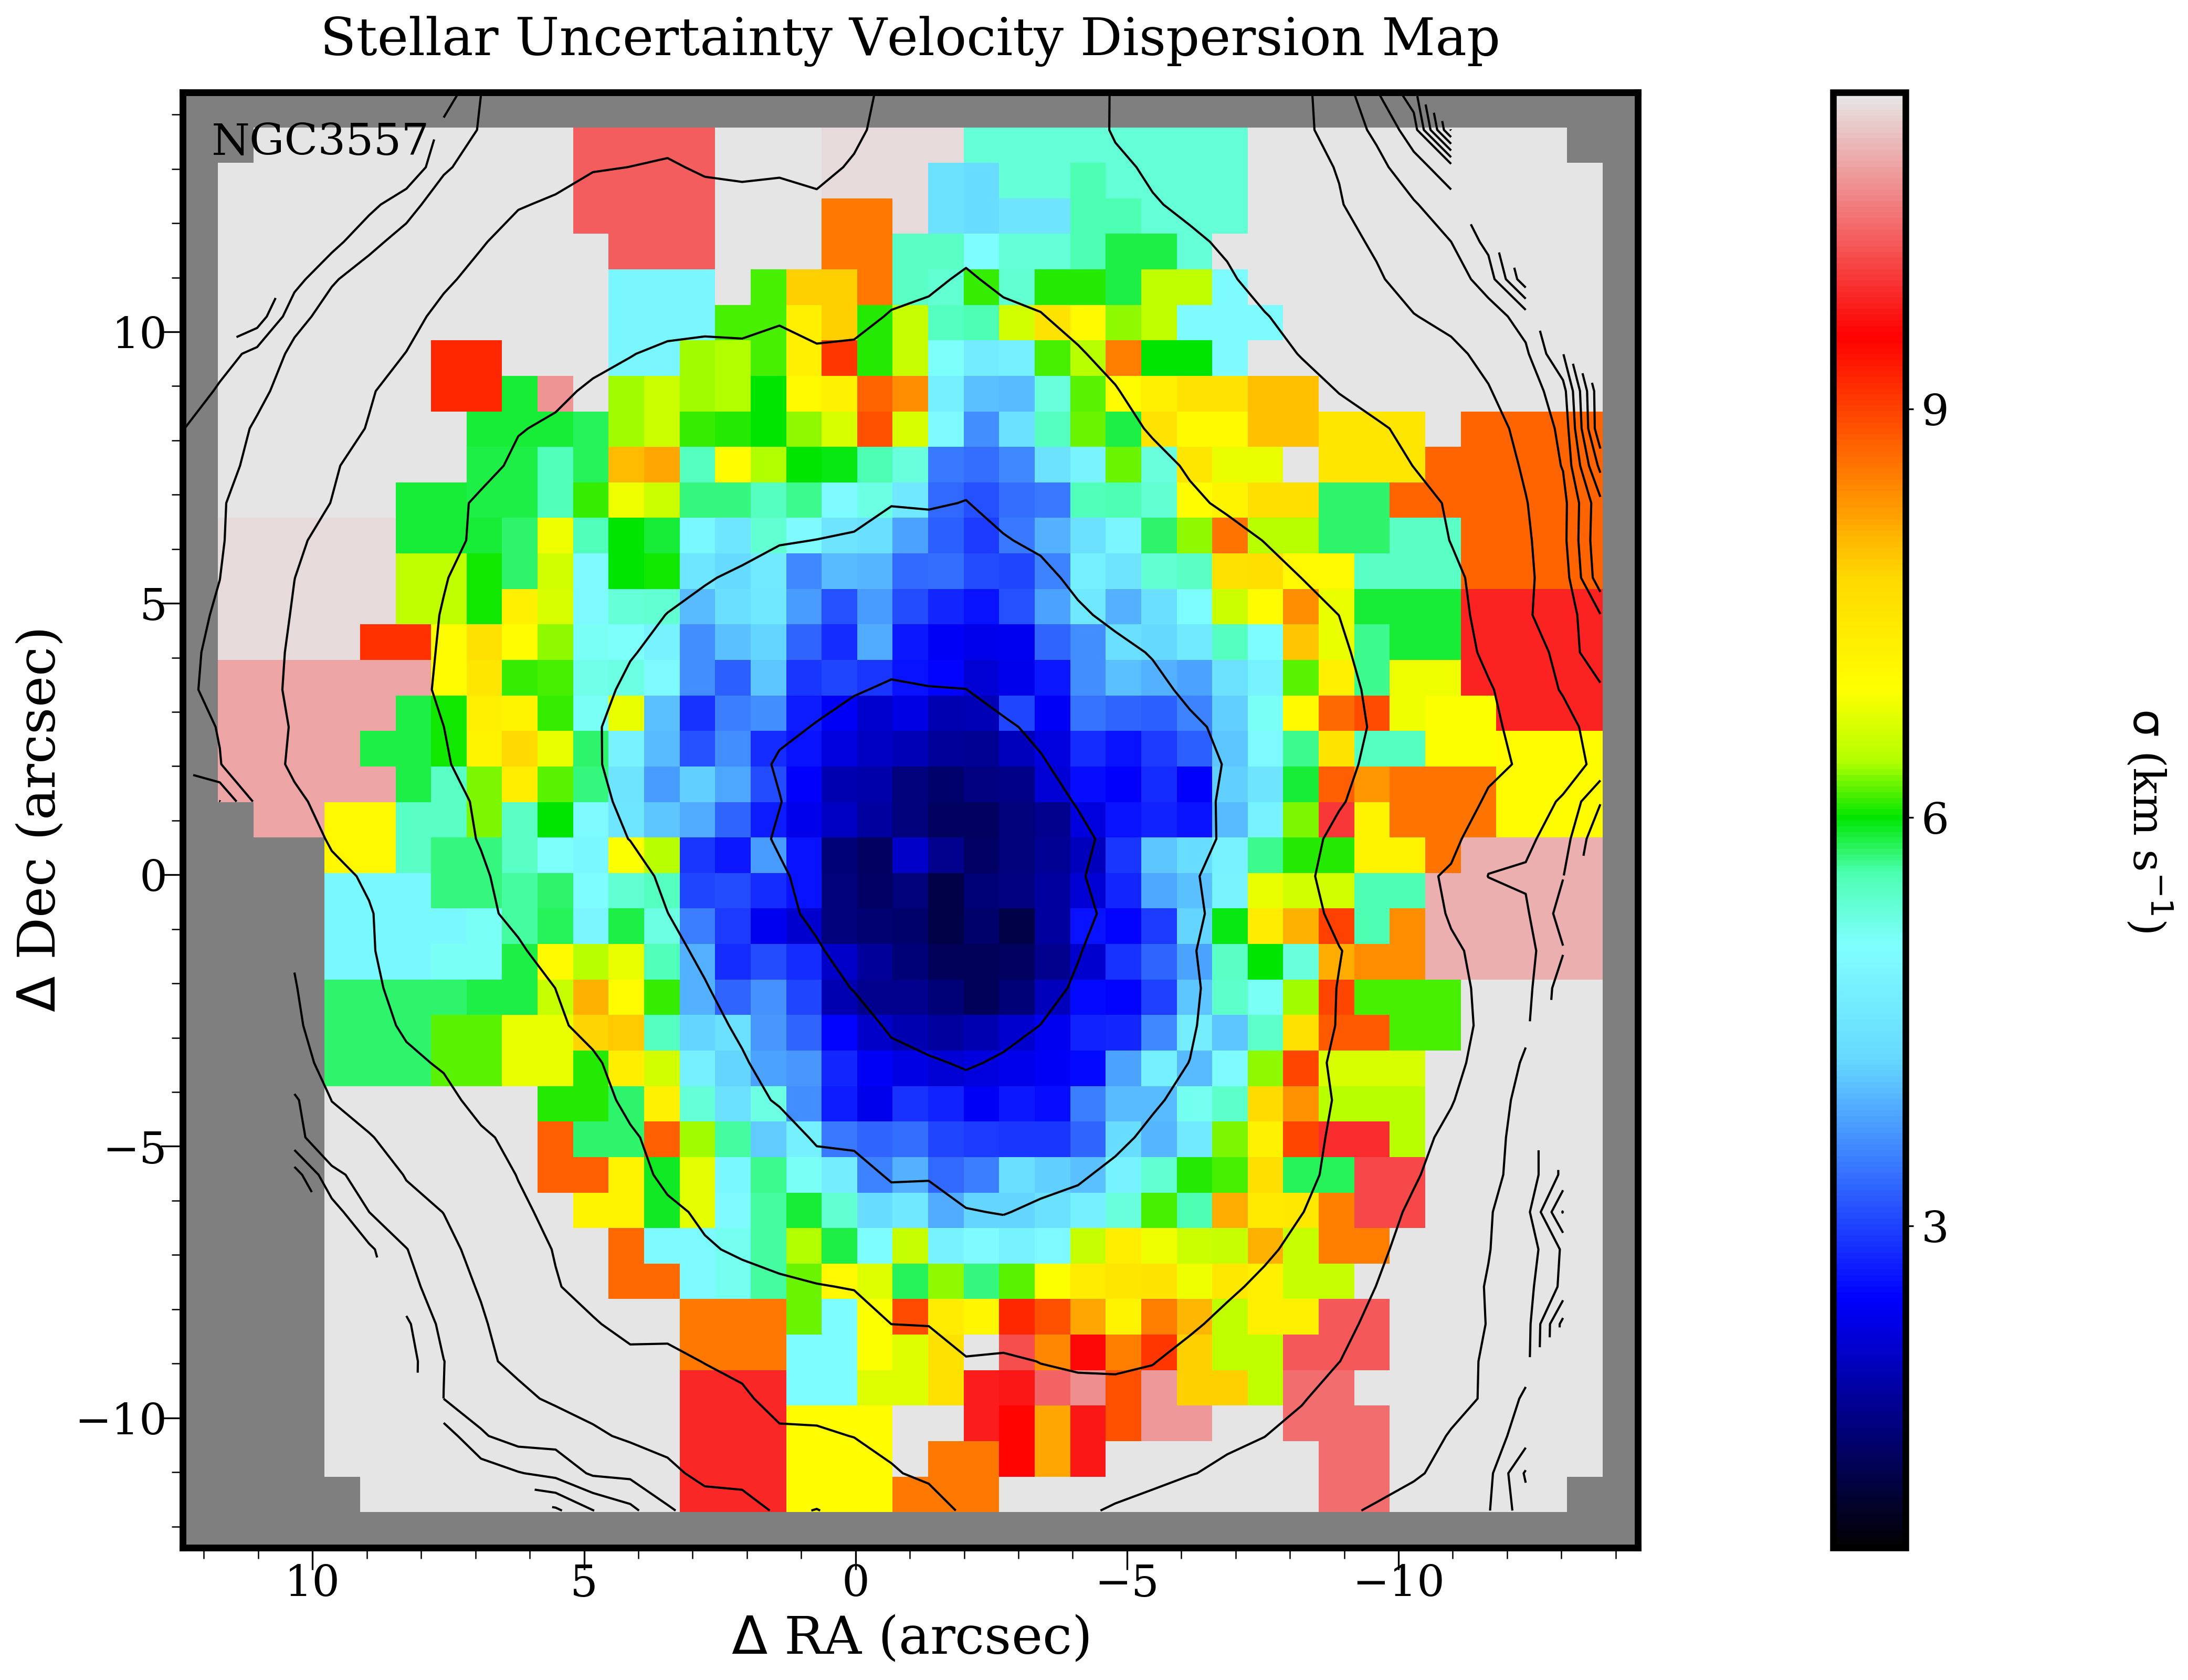
\includegraphics[width=0.245\textwidth]{Vmaps/ngc3557_stellar_sigma_uncert.png}
      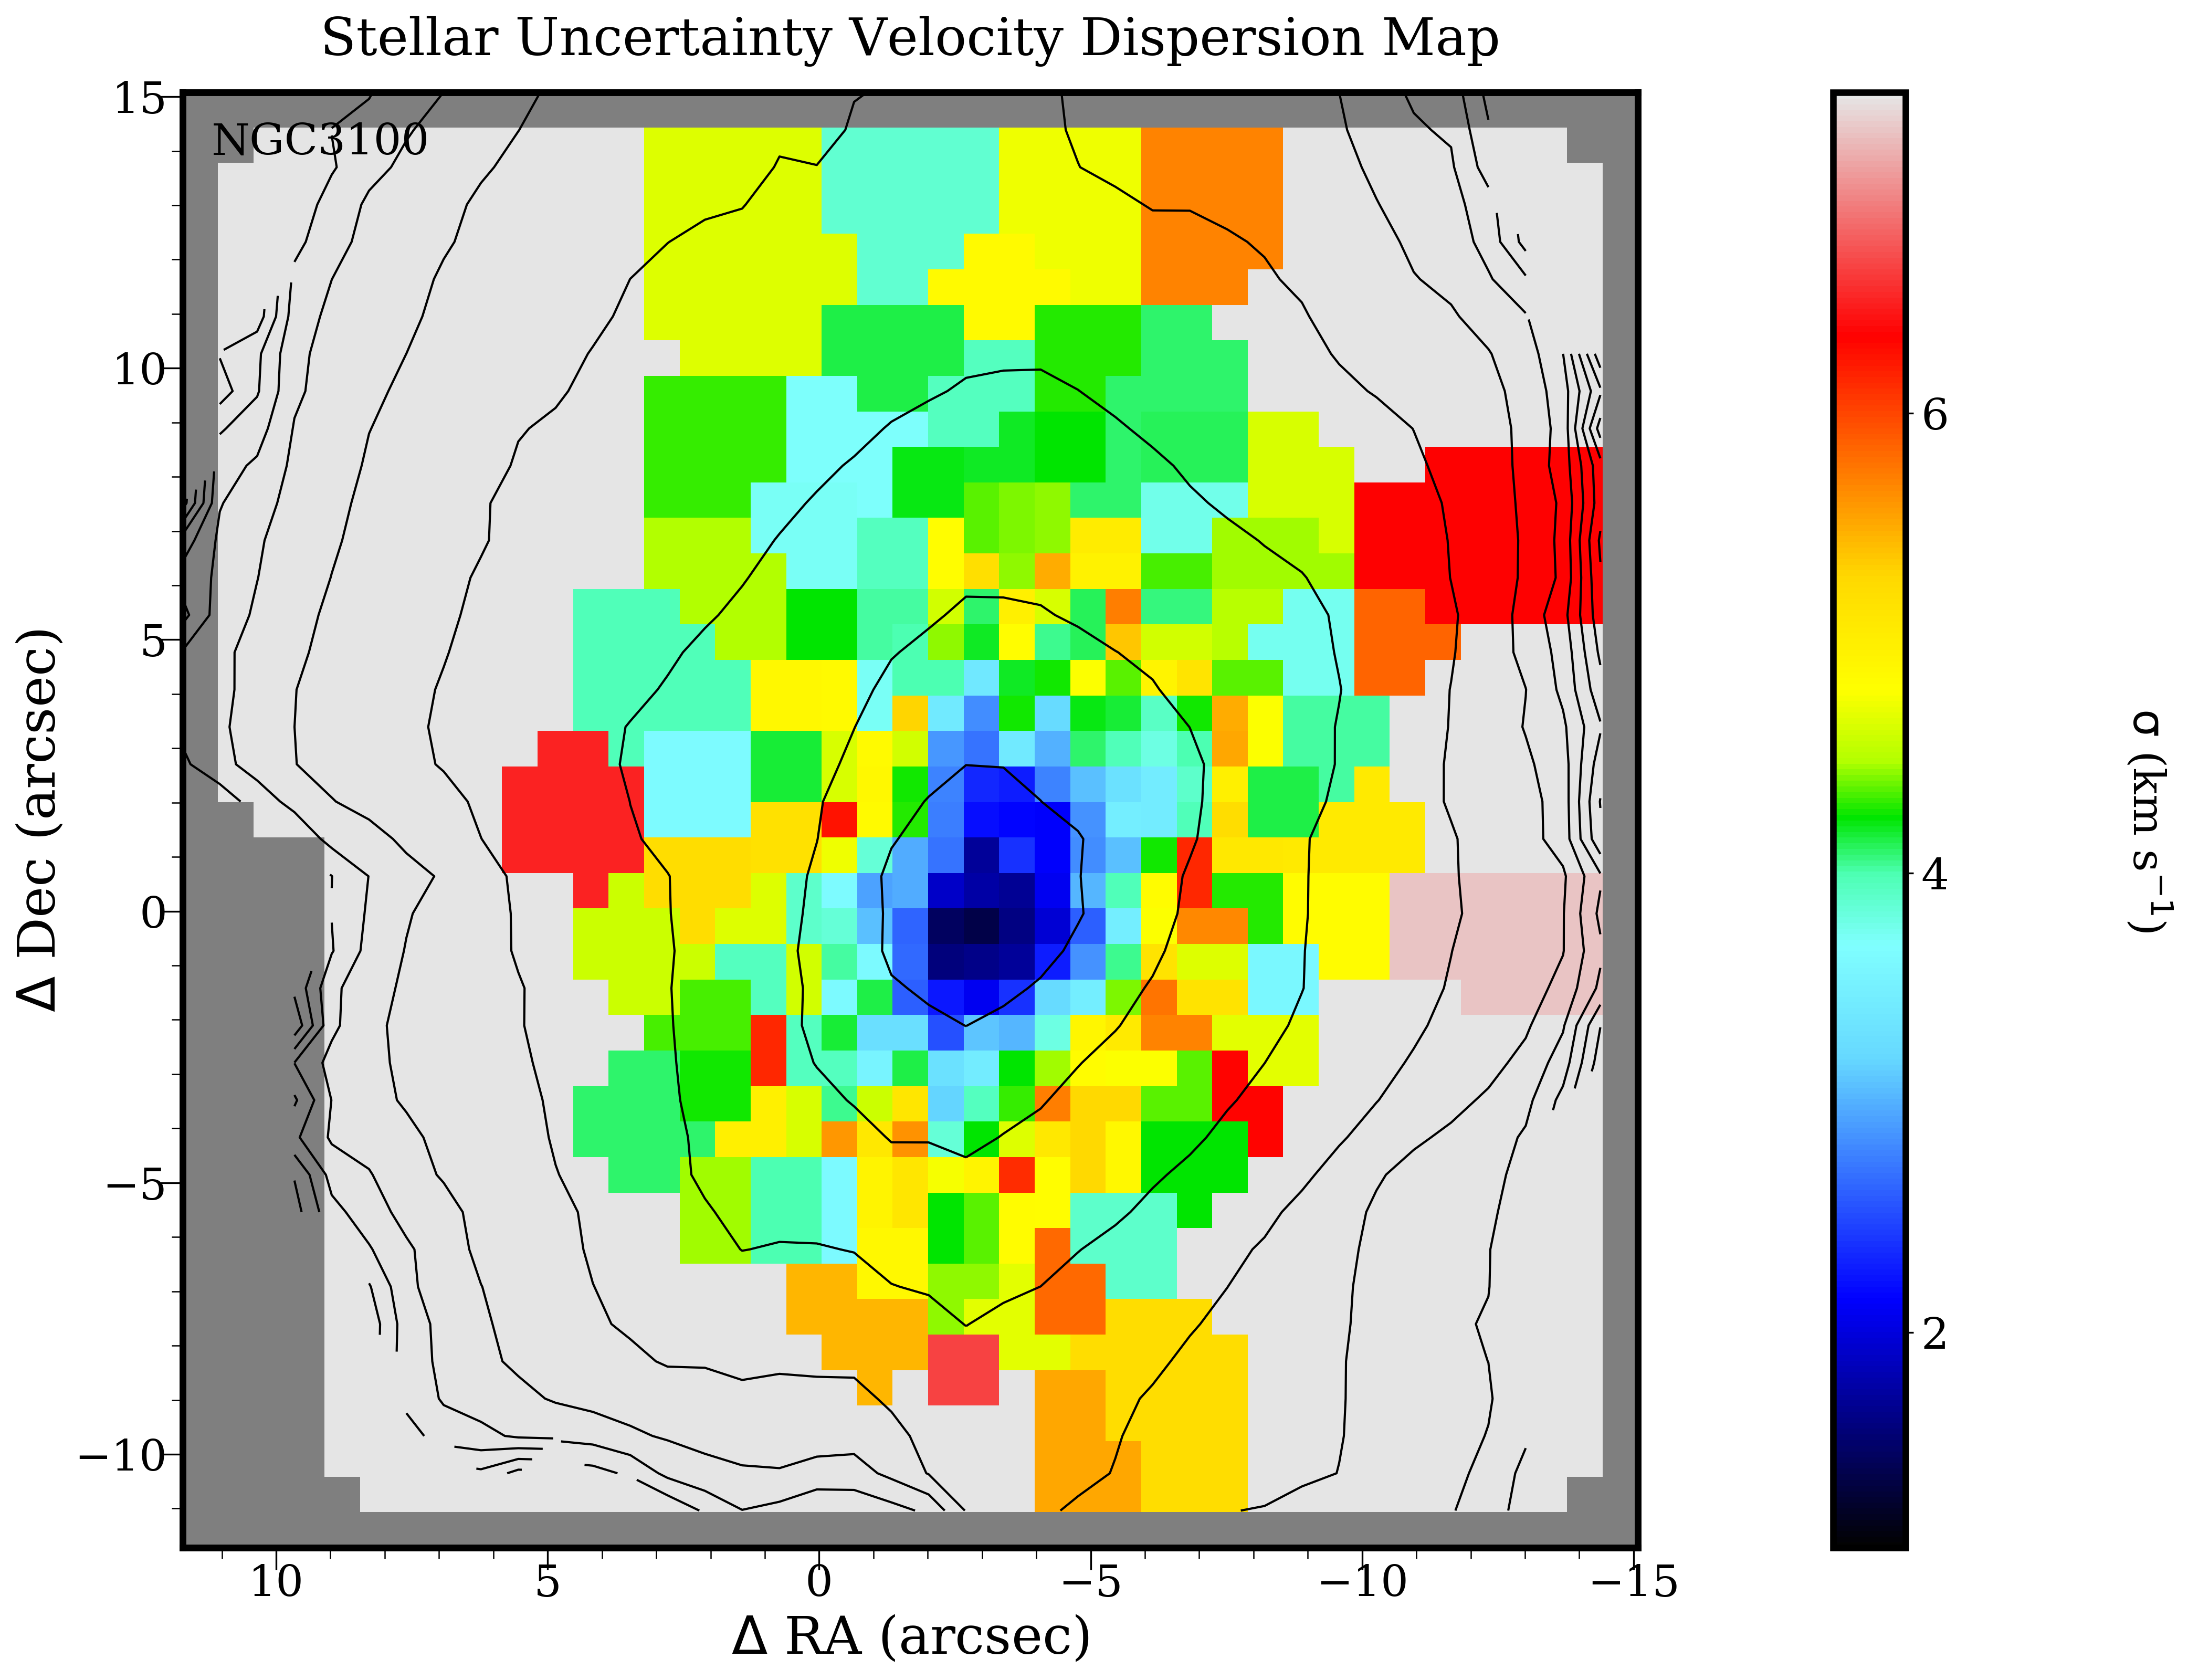
\includegraphics[width=0.245\textwidth]{Vmaps/ngc3100_stellar_sigma_uncert.png}
      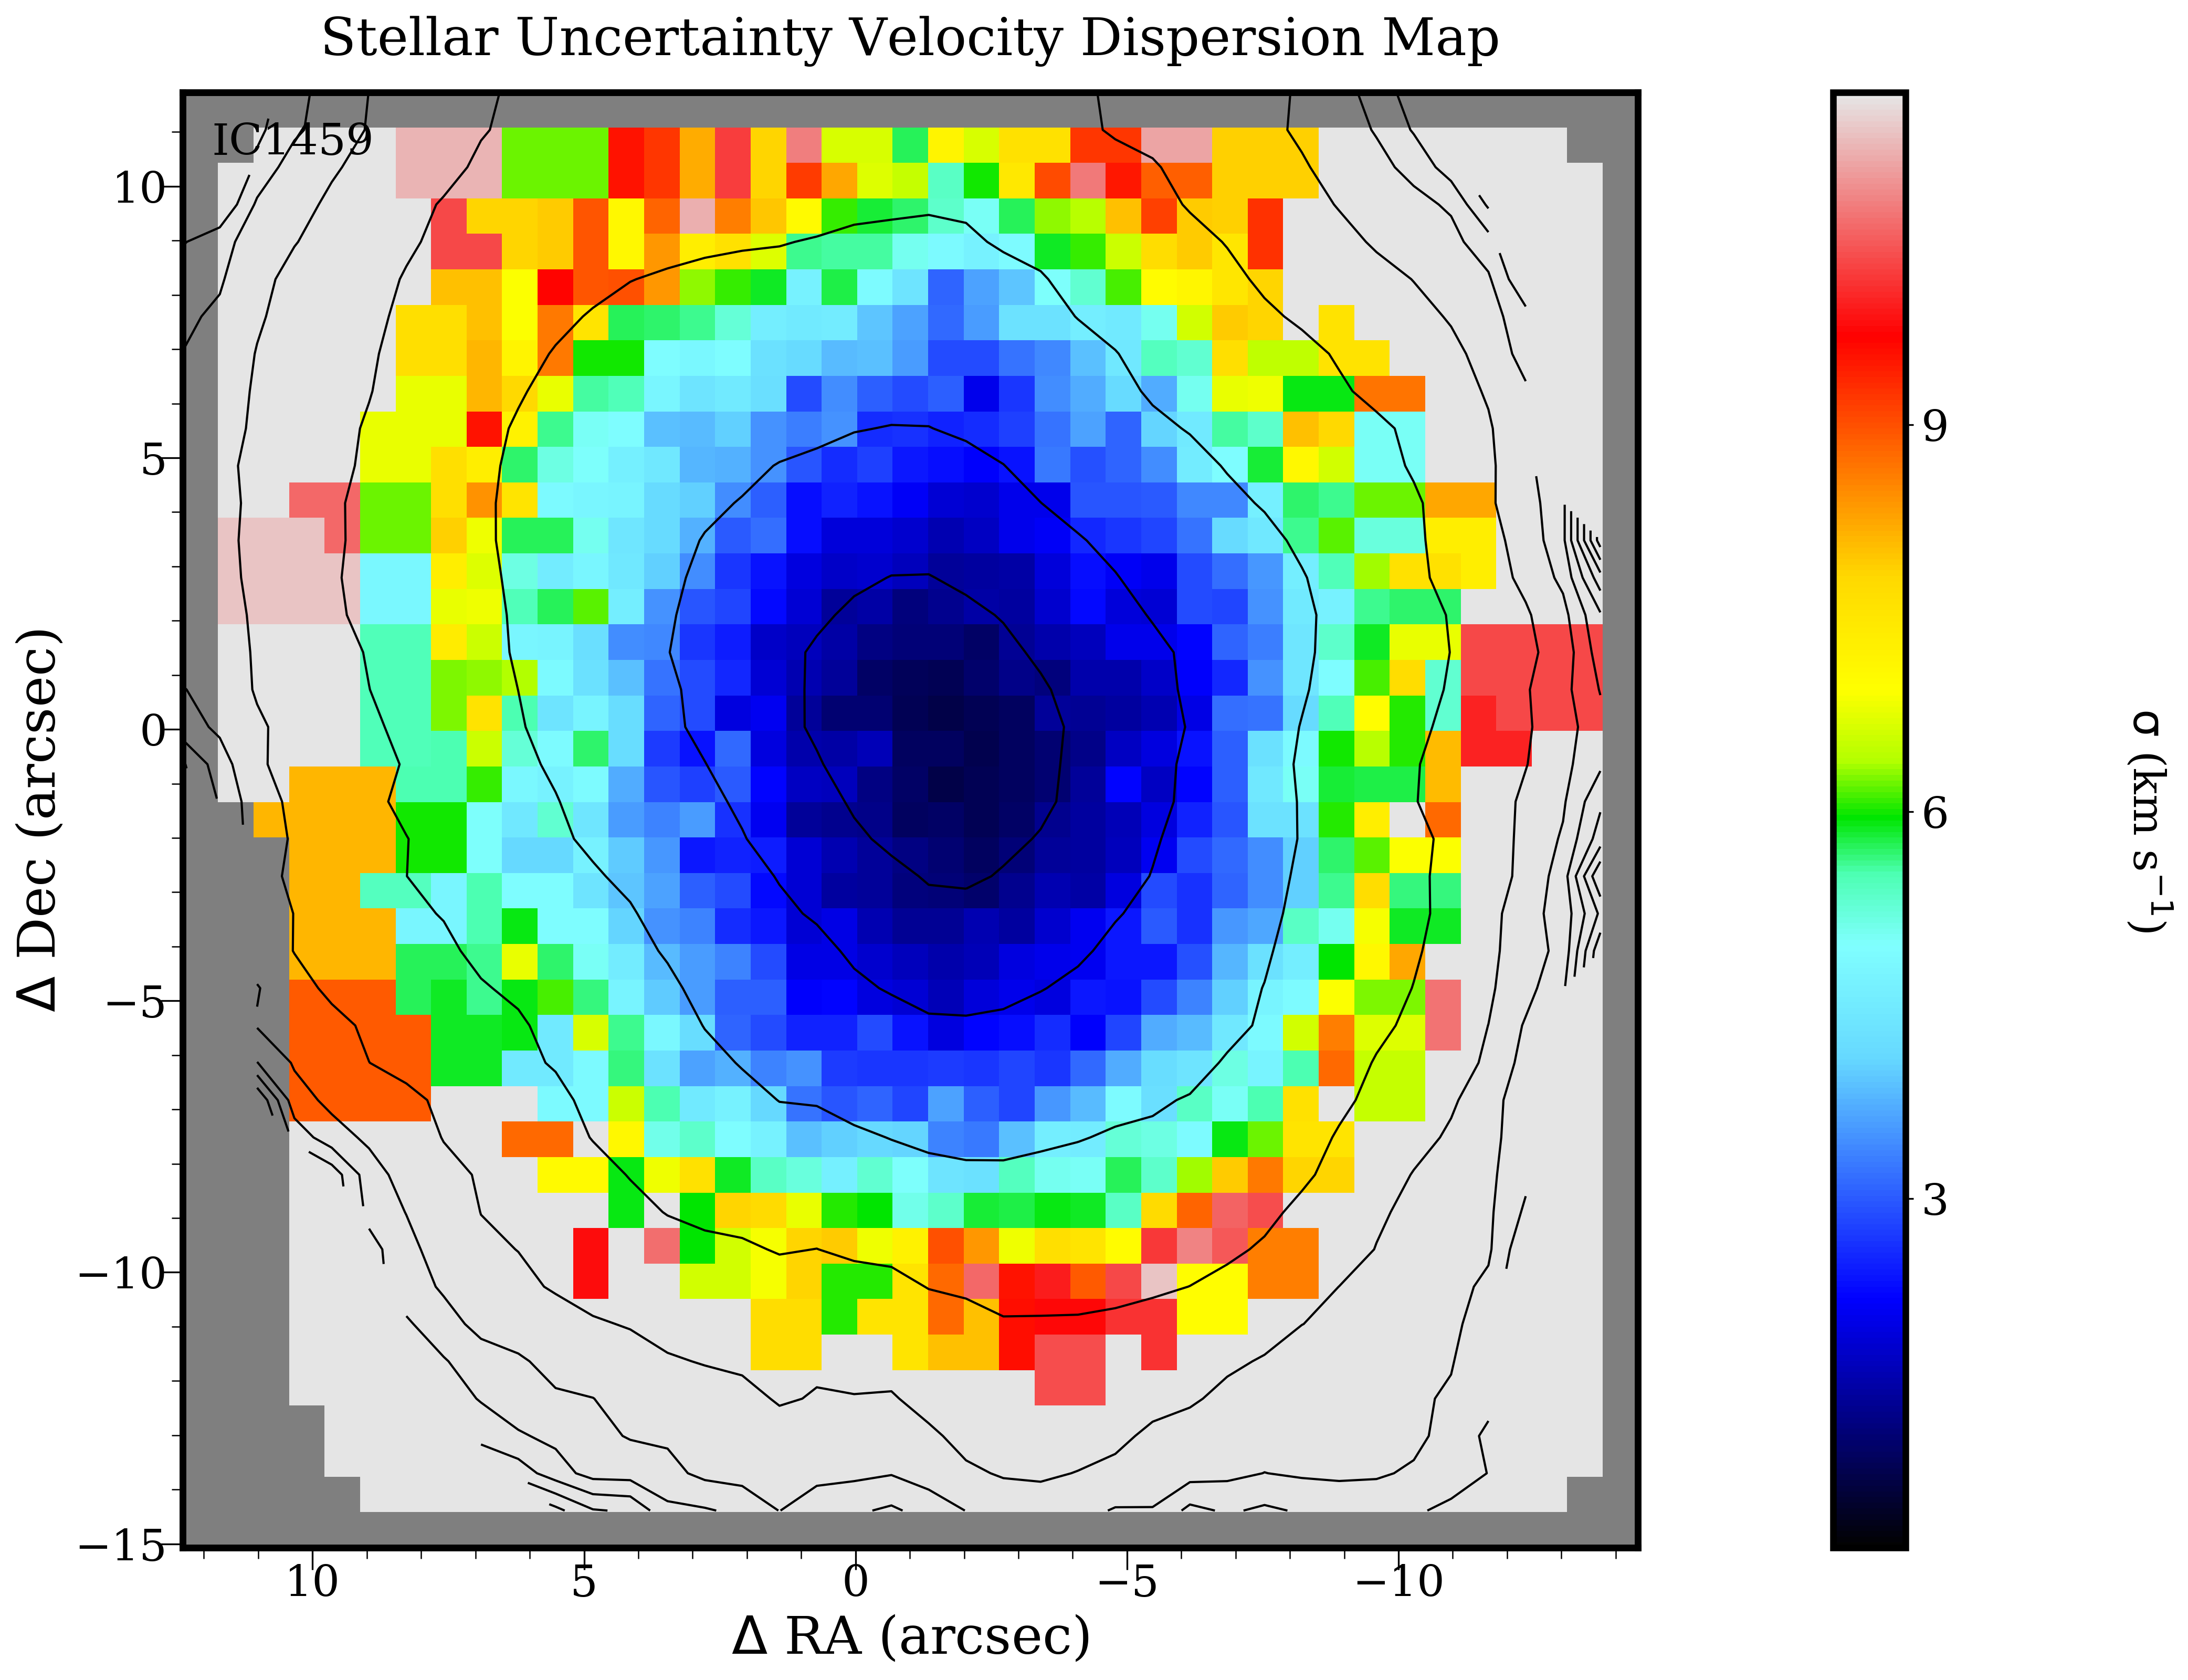
\includegraphics[width=0.245\textwidth]{Vmaps/ic1459_stellar_sigma_uncert.png}
      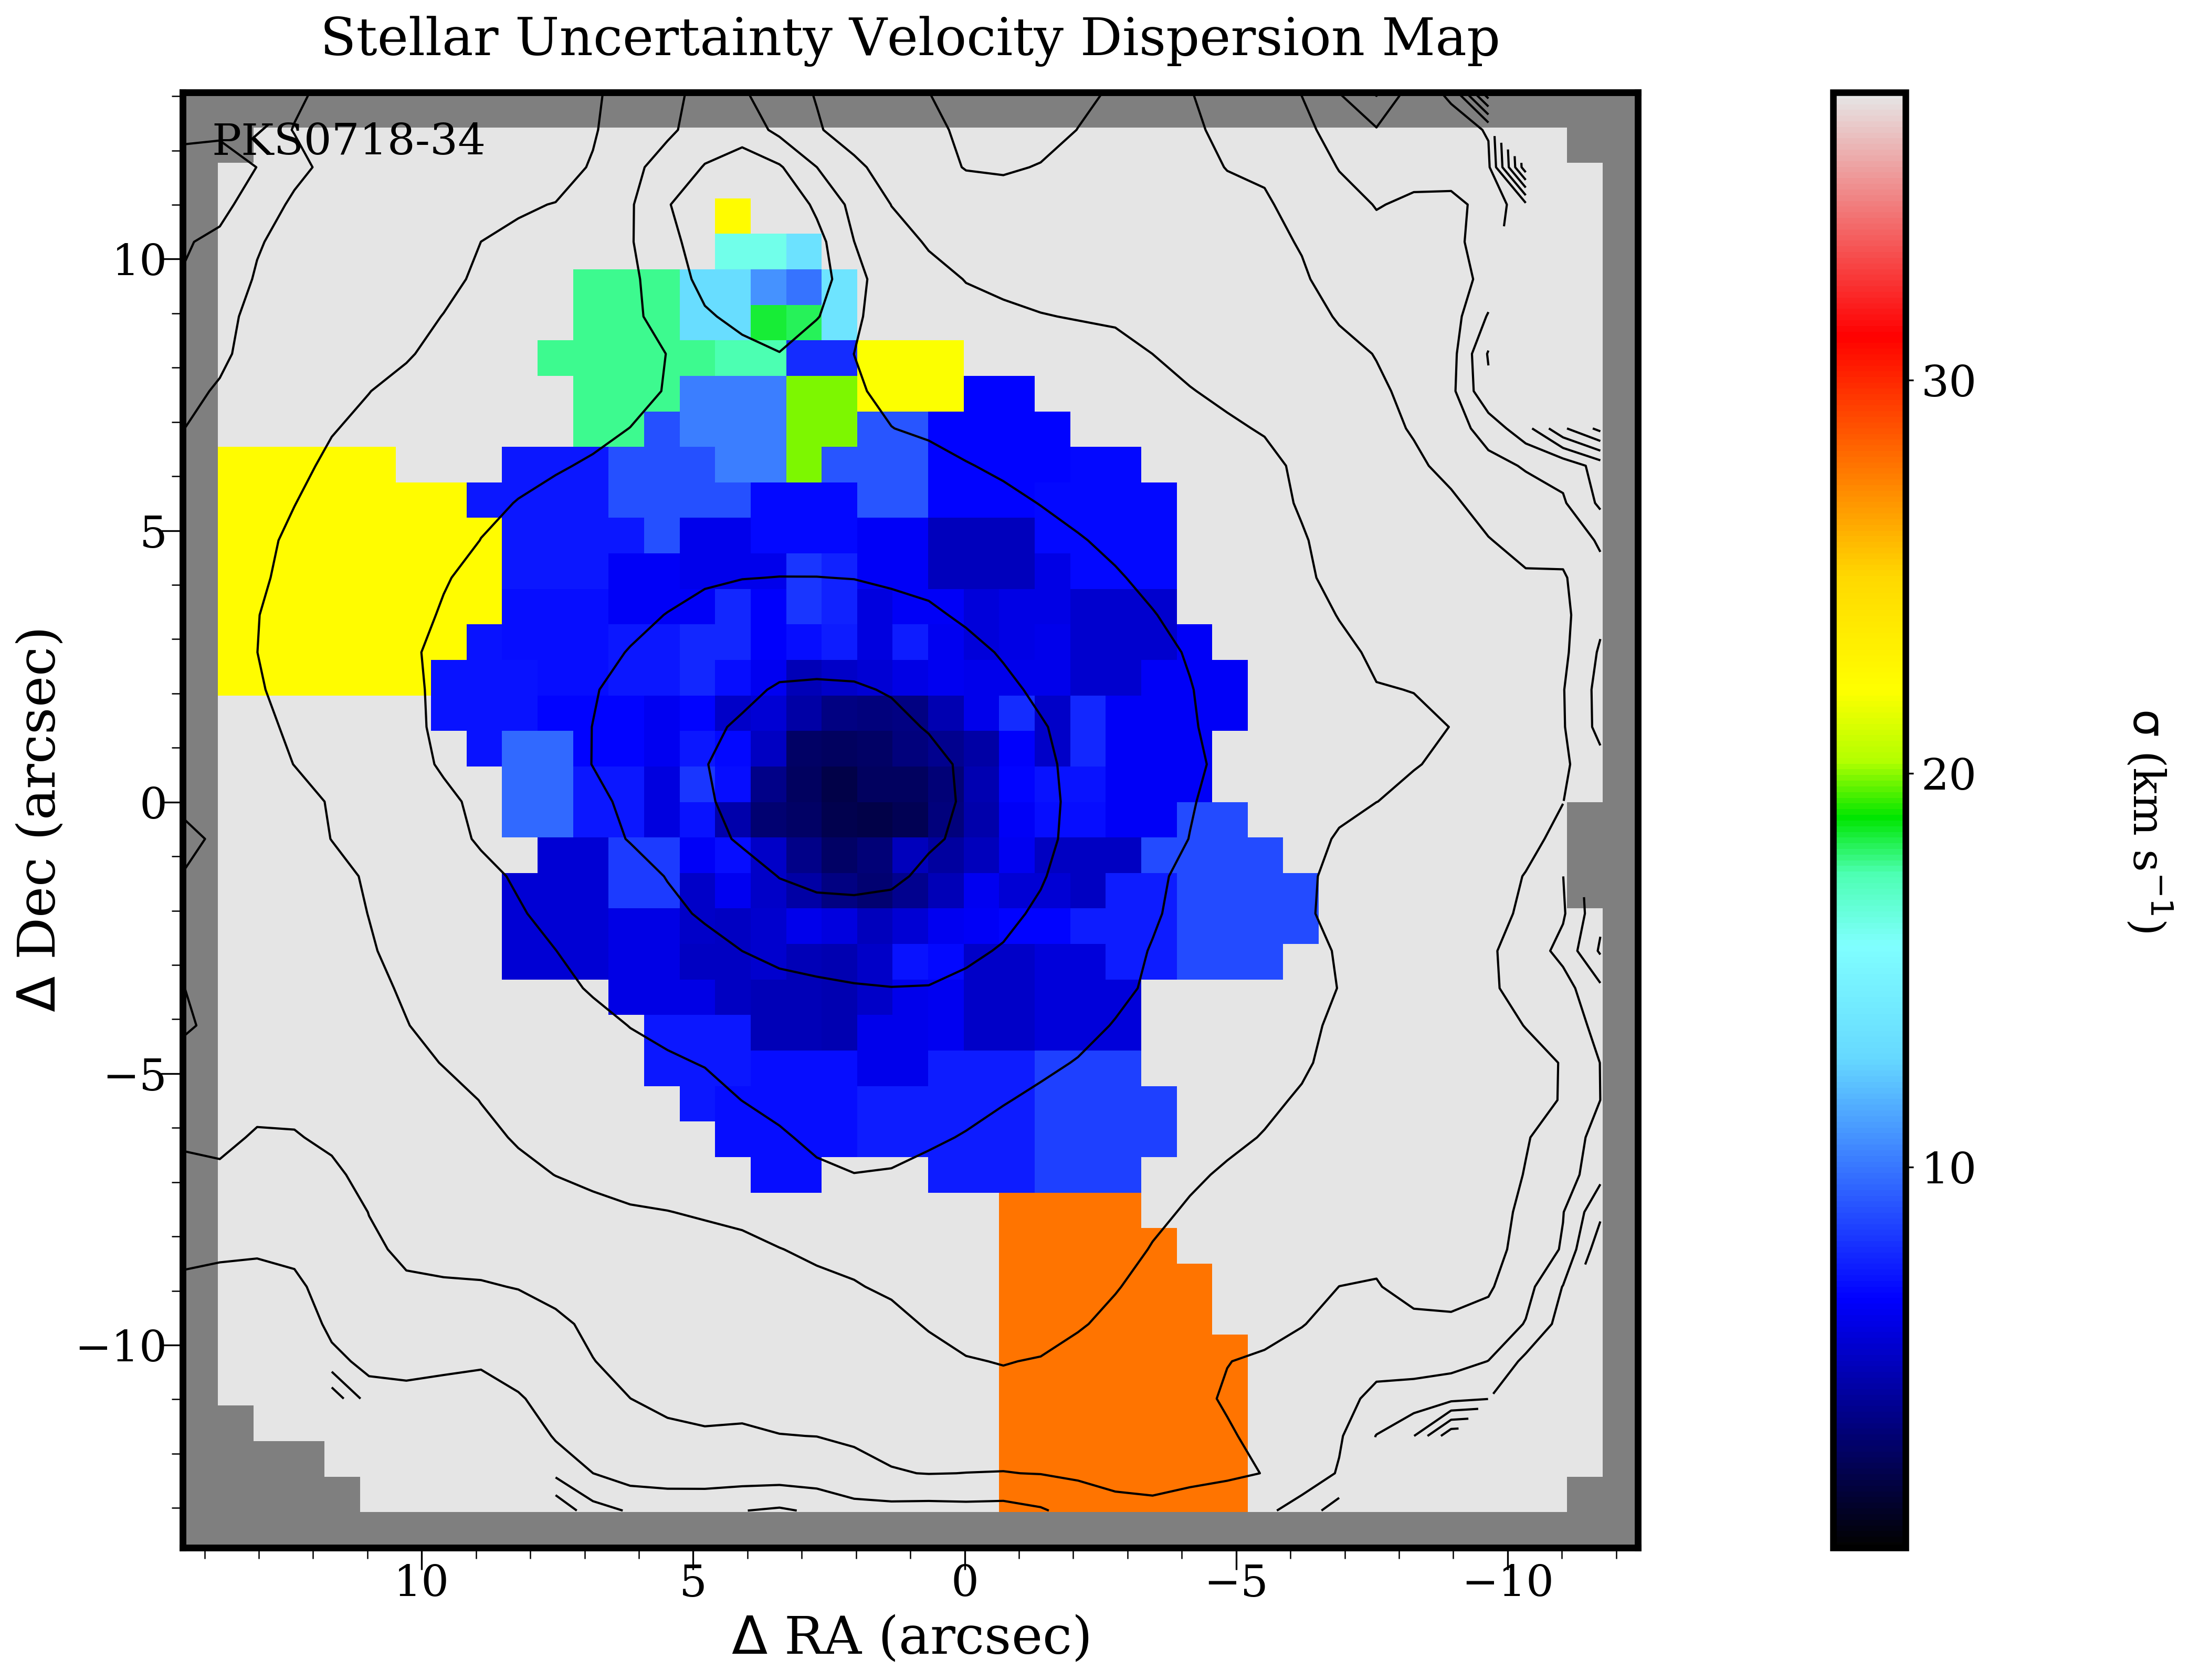
\includegraphics[width=0.245\textwidth]{Vmaps/pks0718-34_stellar_sigma_uncert.png}
      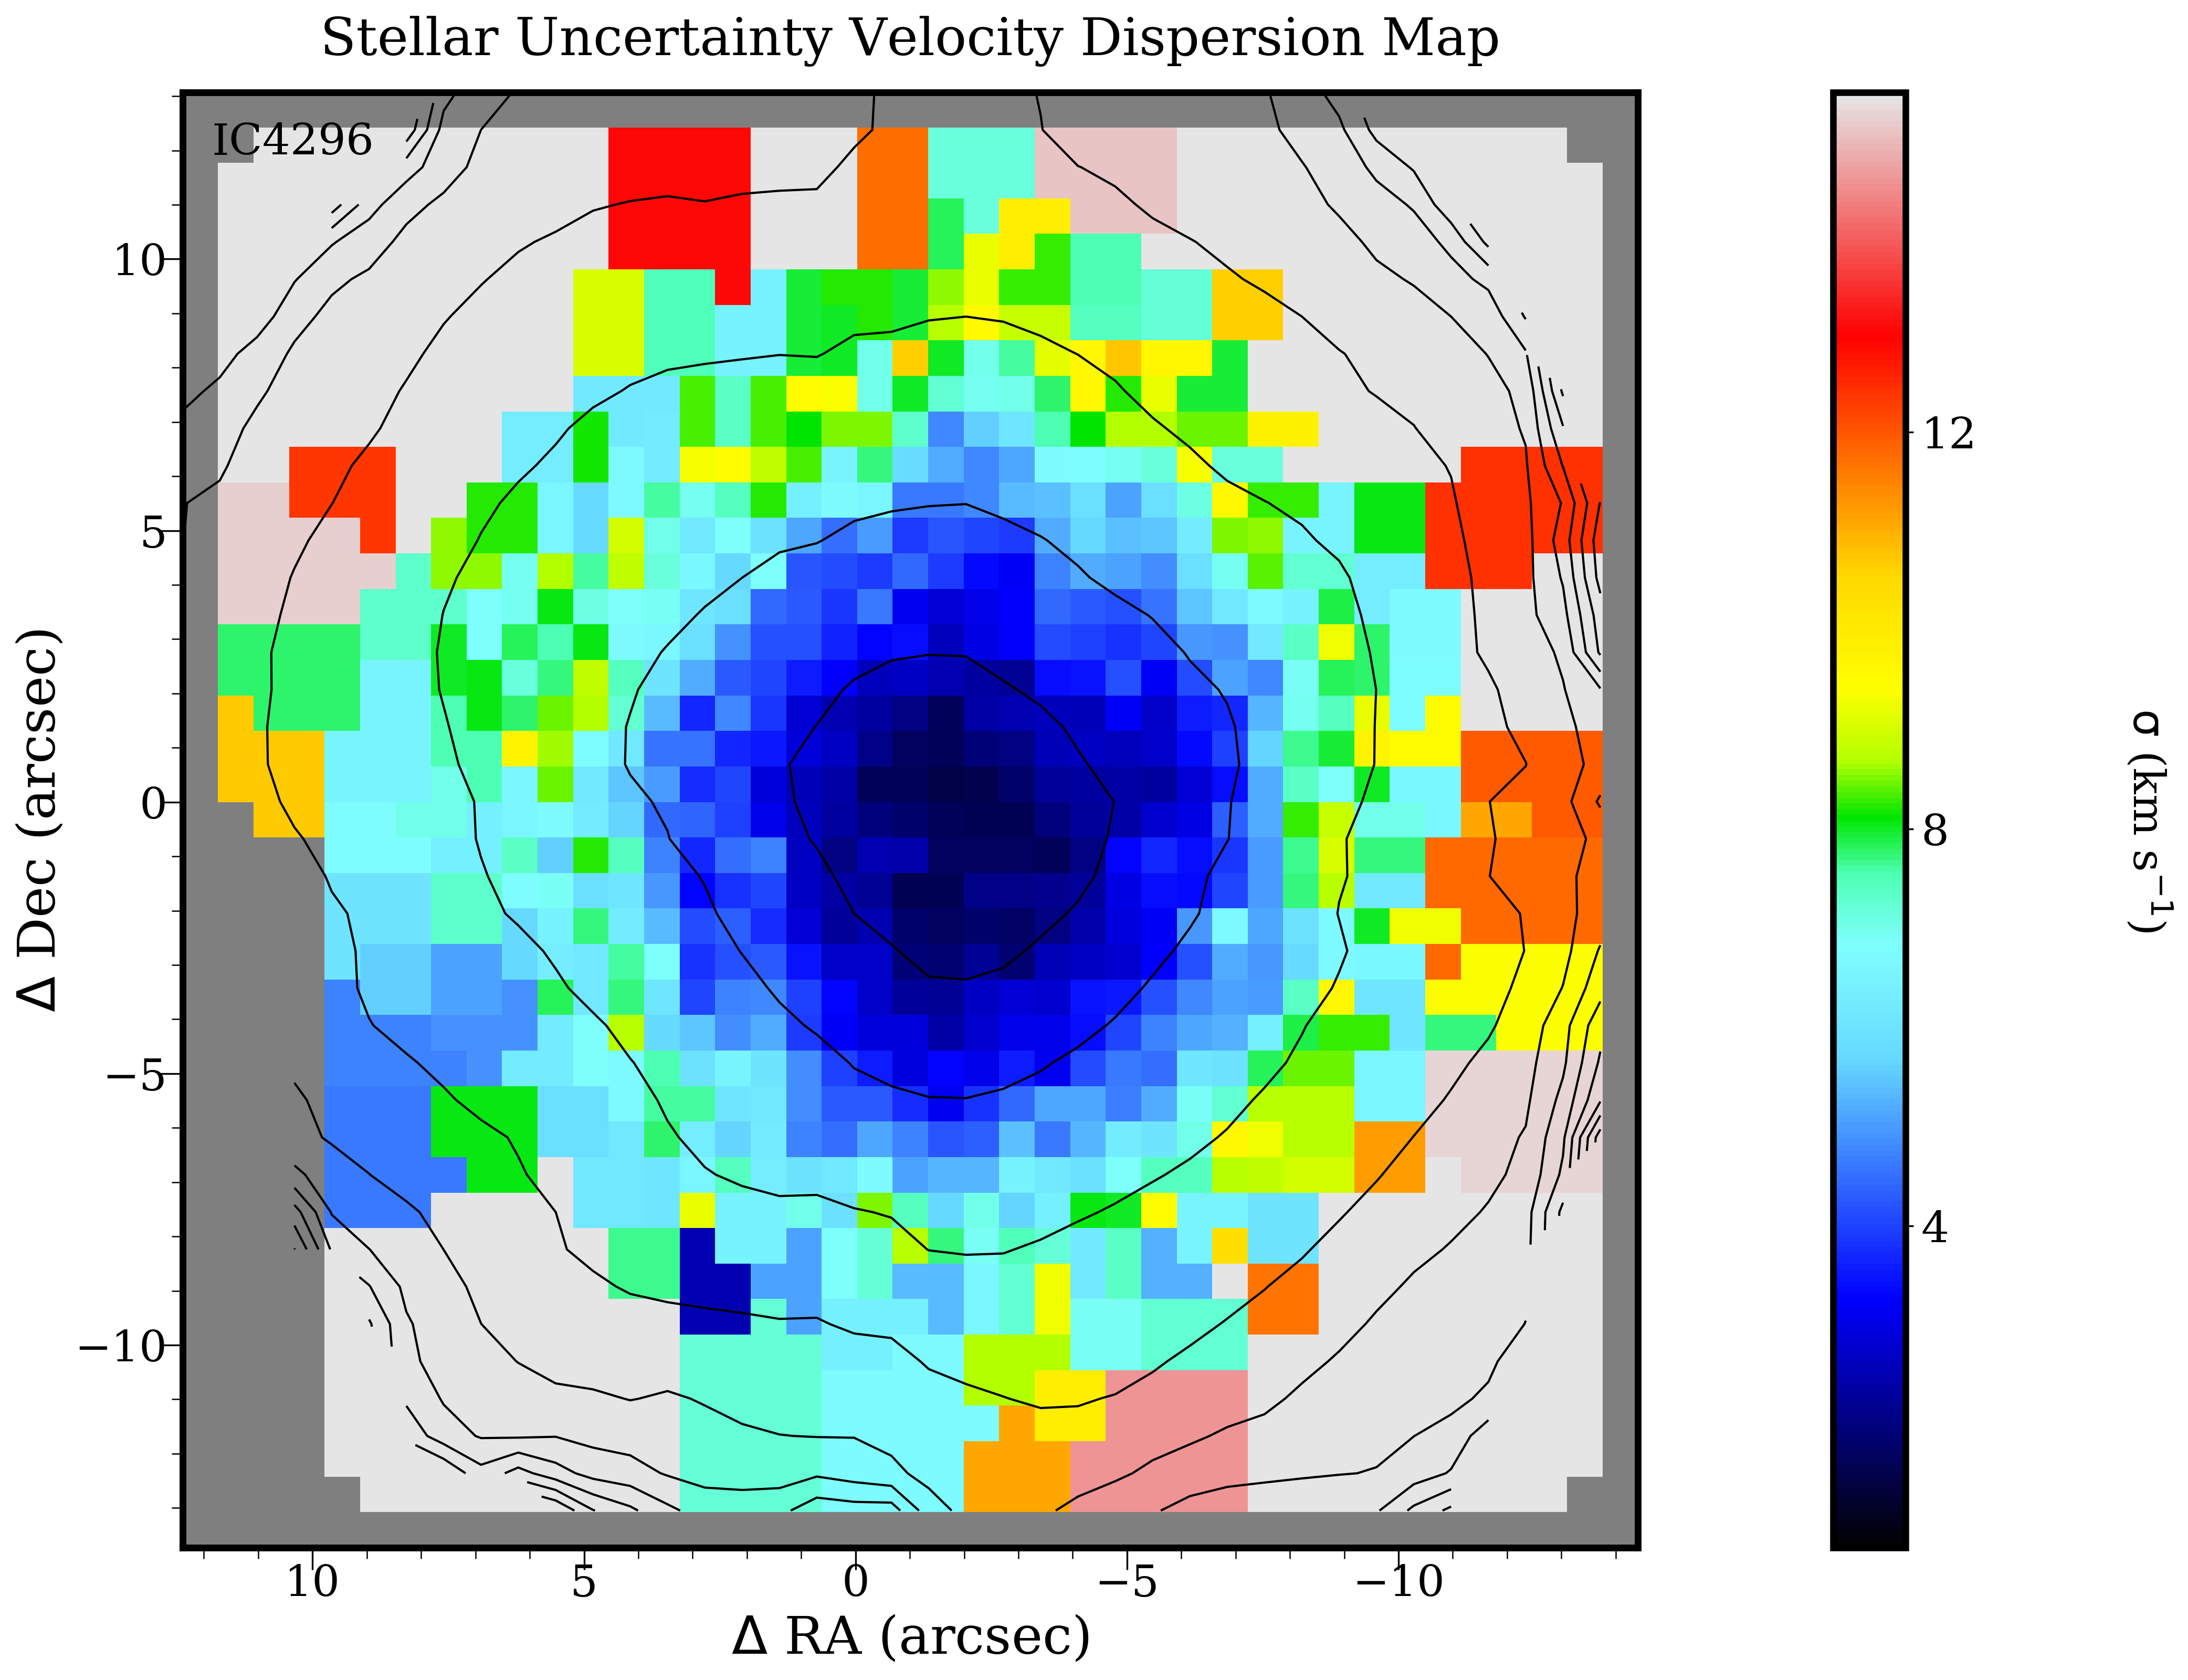
\includegraphics[width=0.245\textwidth]{Vmaps/ic4296_stellar_sigma_uncert.png}
      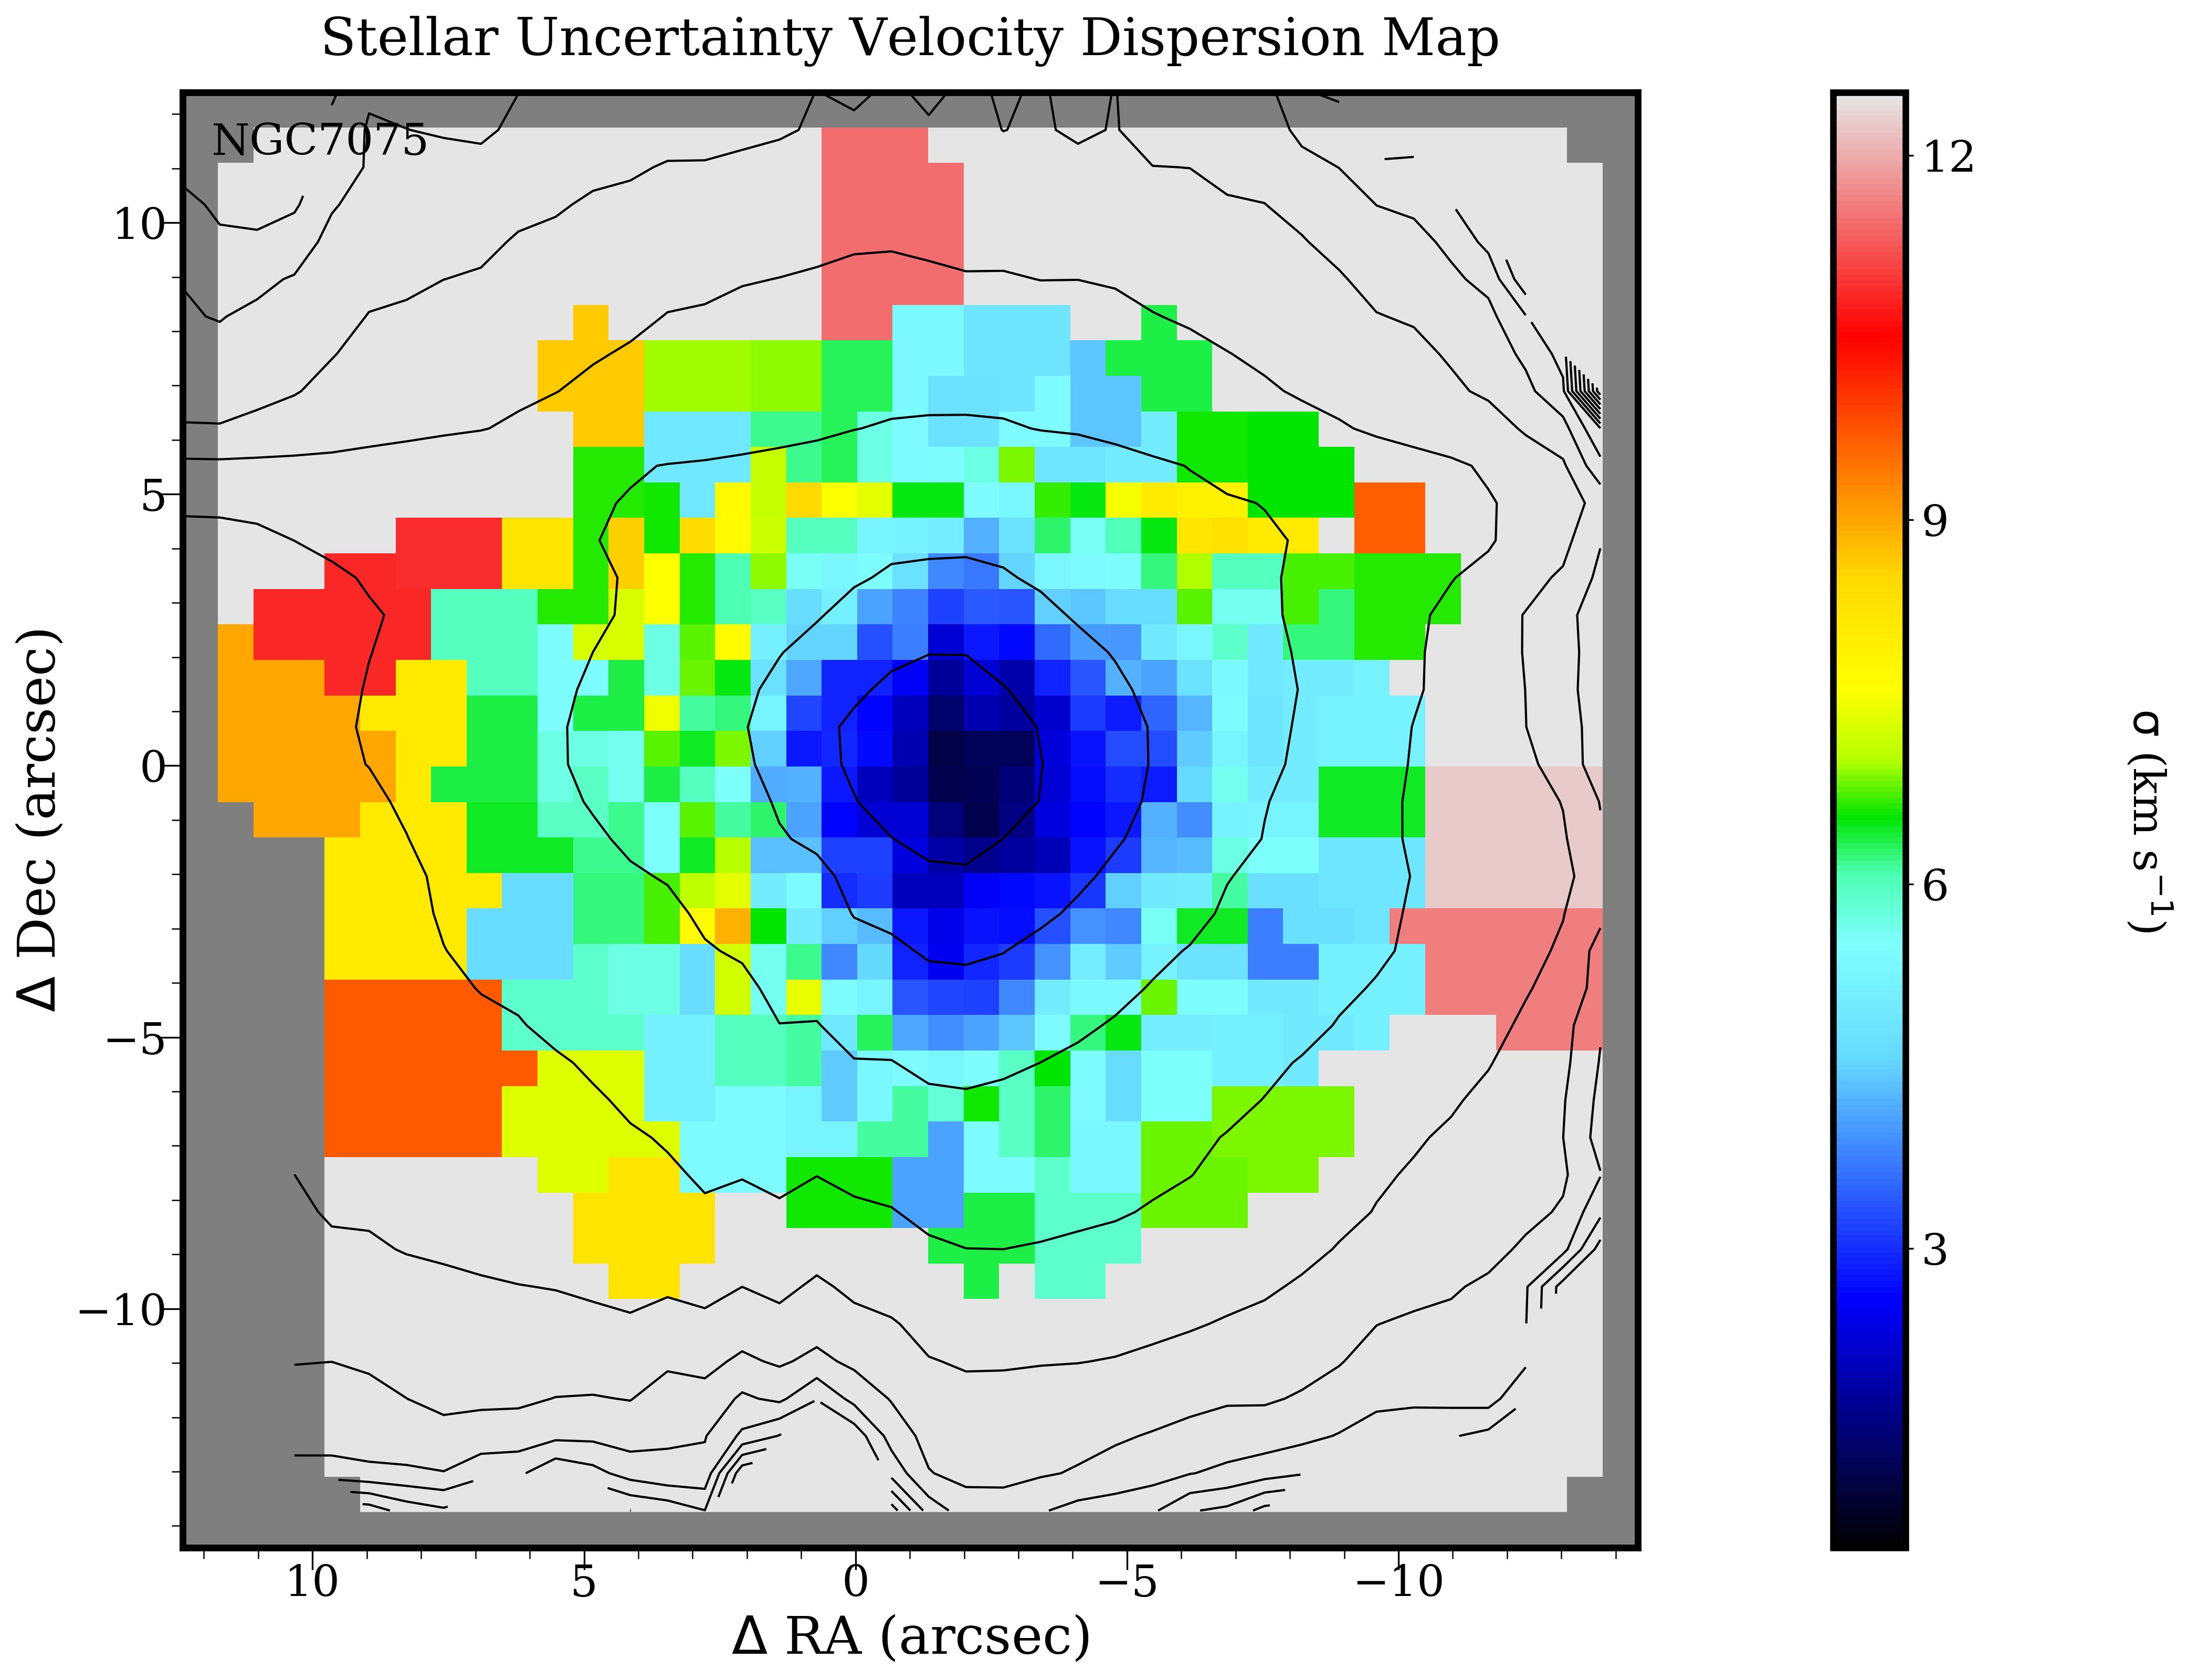
\includegraphics[width=0.245\textwidth]{Vmaps/ngc7075_stellar_sigma_uncert.png}
      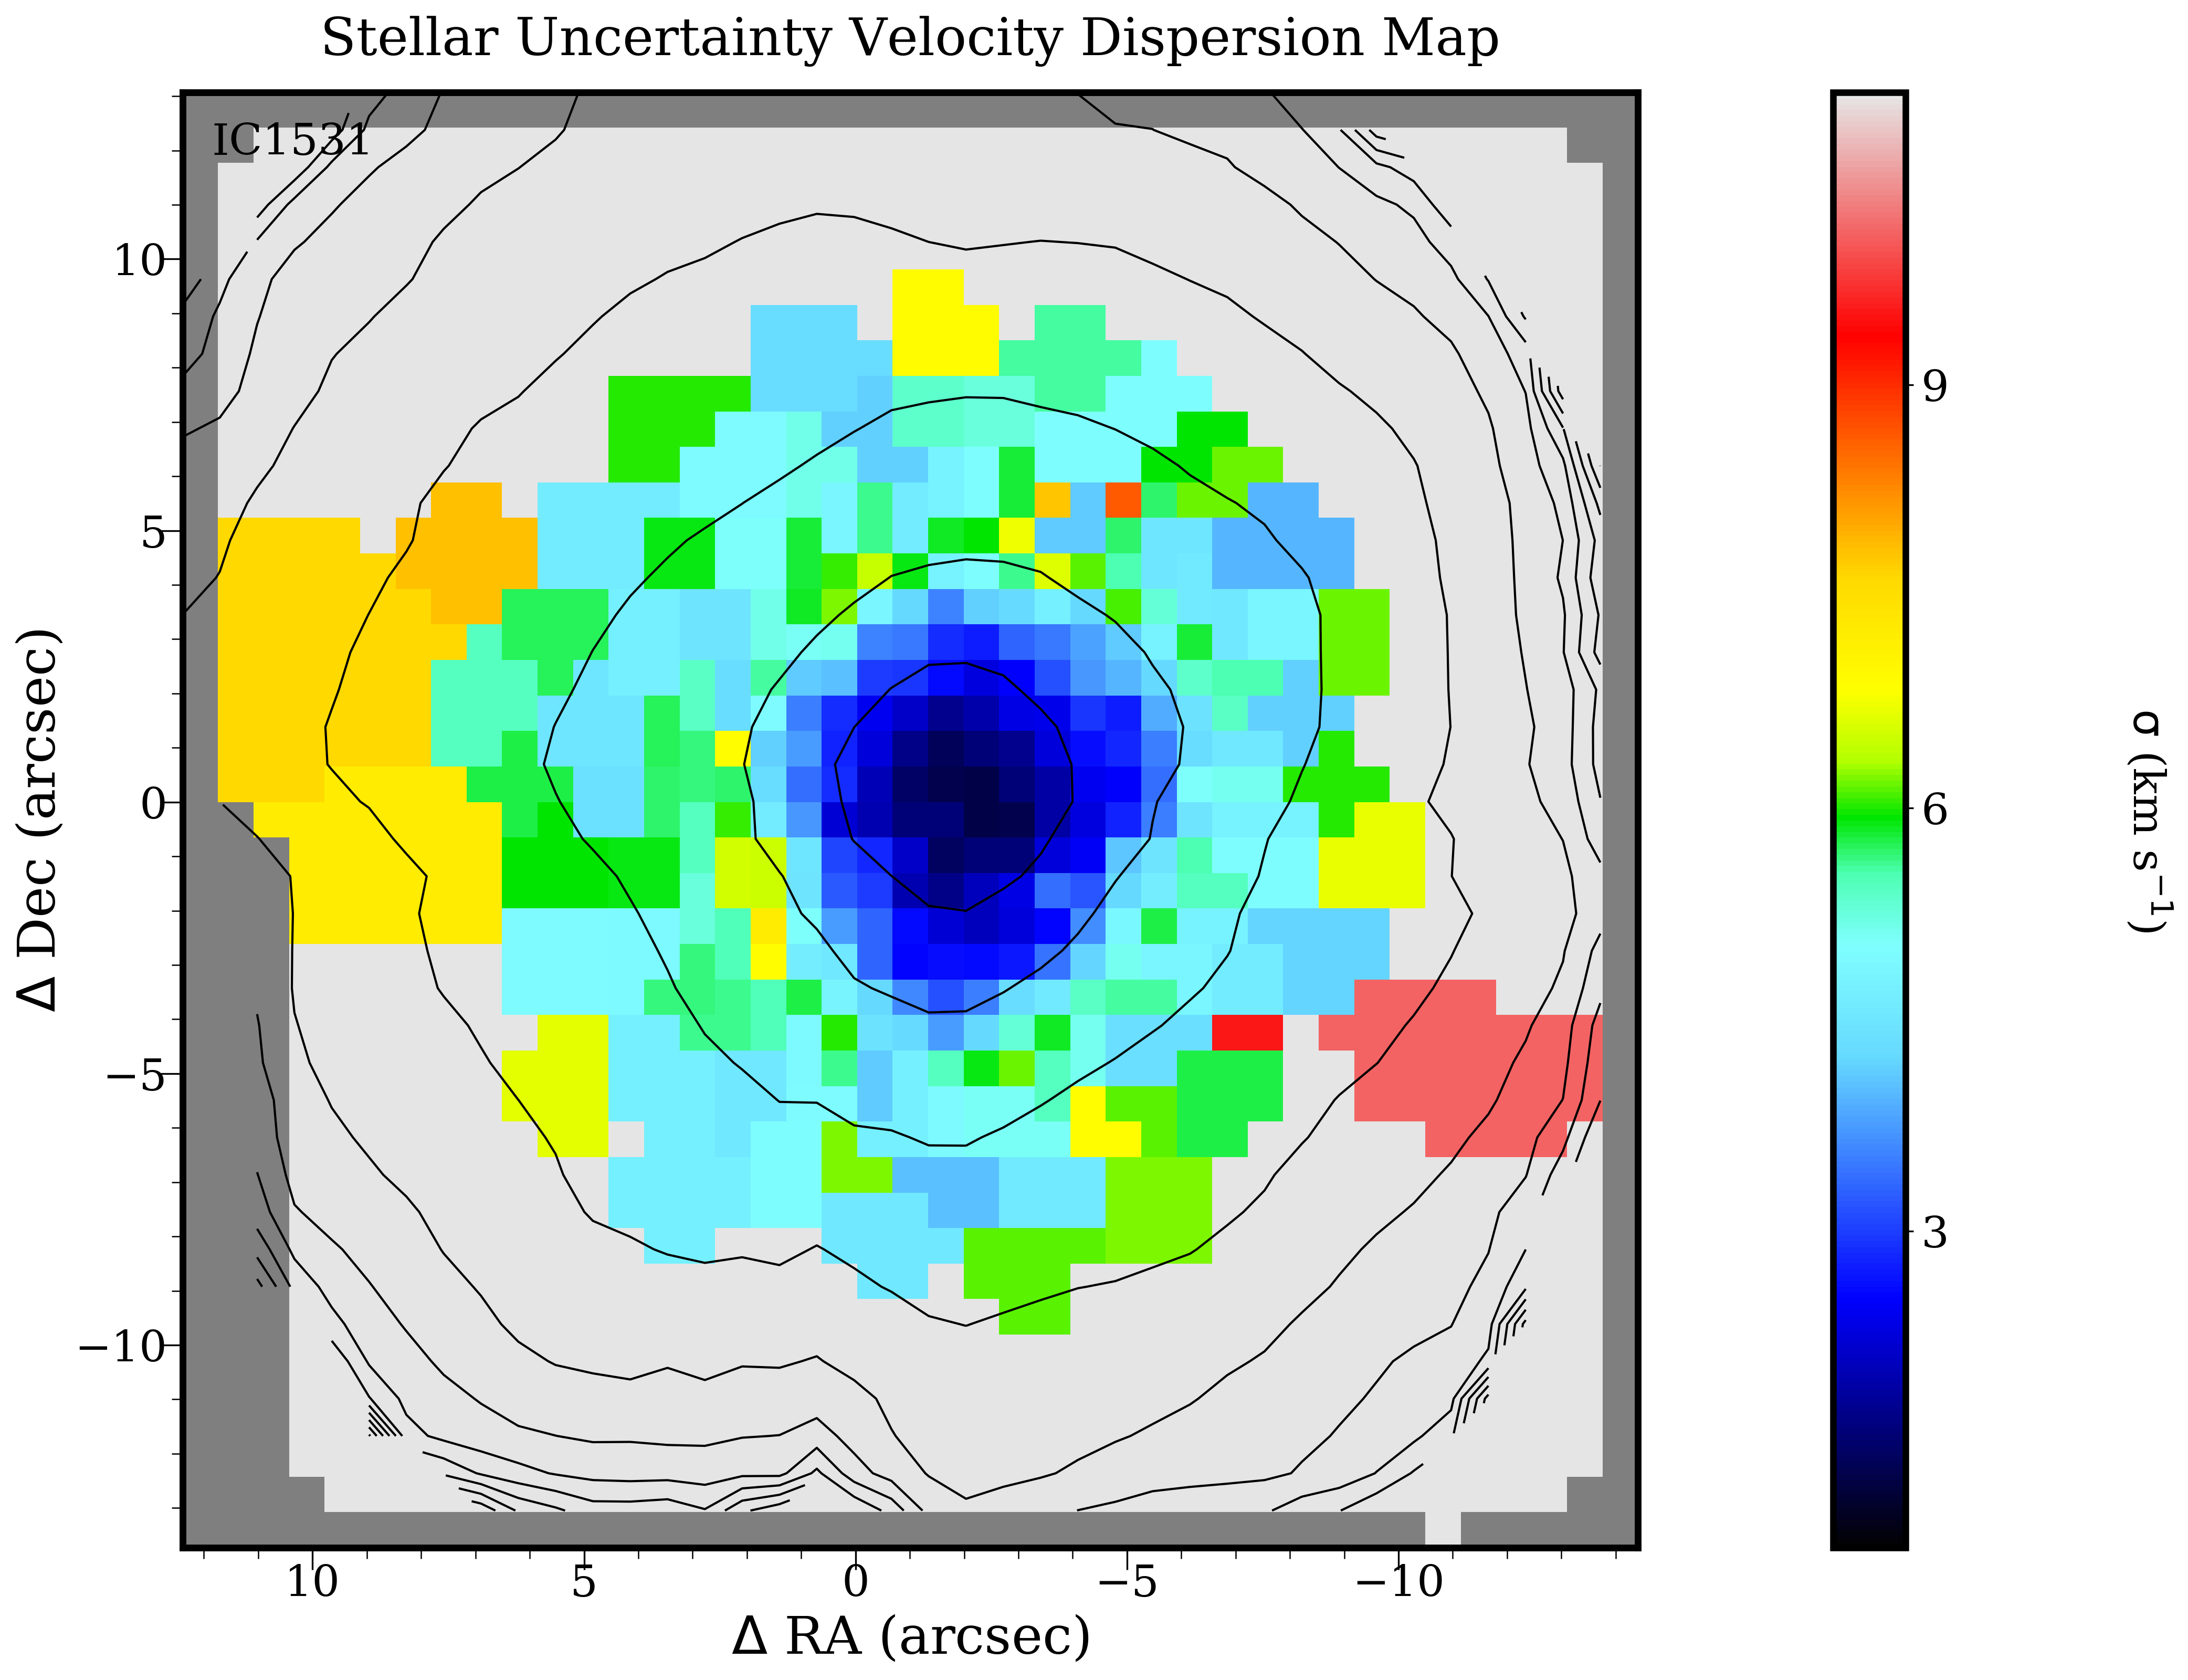
\includegraphics[width=0.245\textwidth]{Vmaps/ic1531_stellar_sigma_uncert.png}
      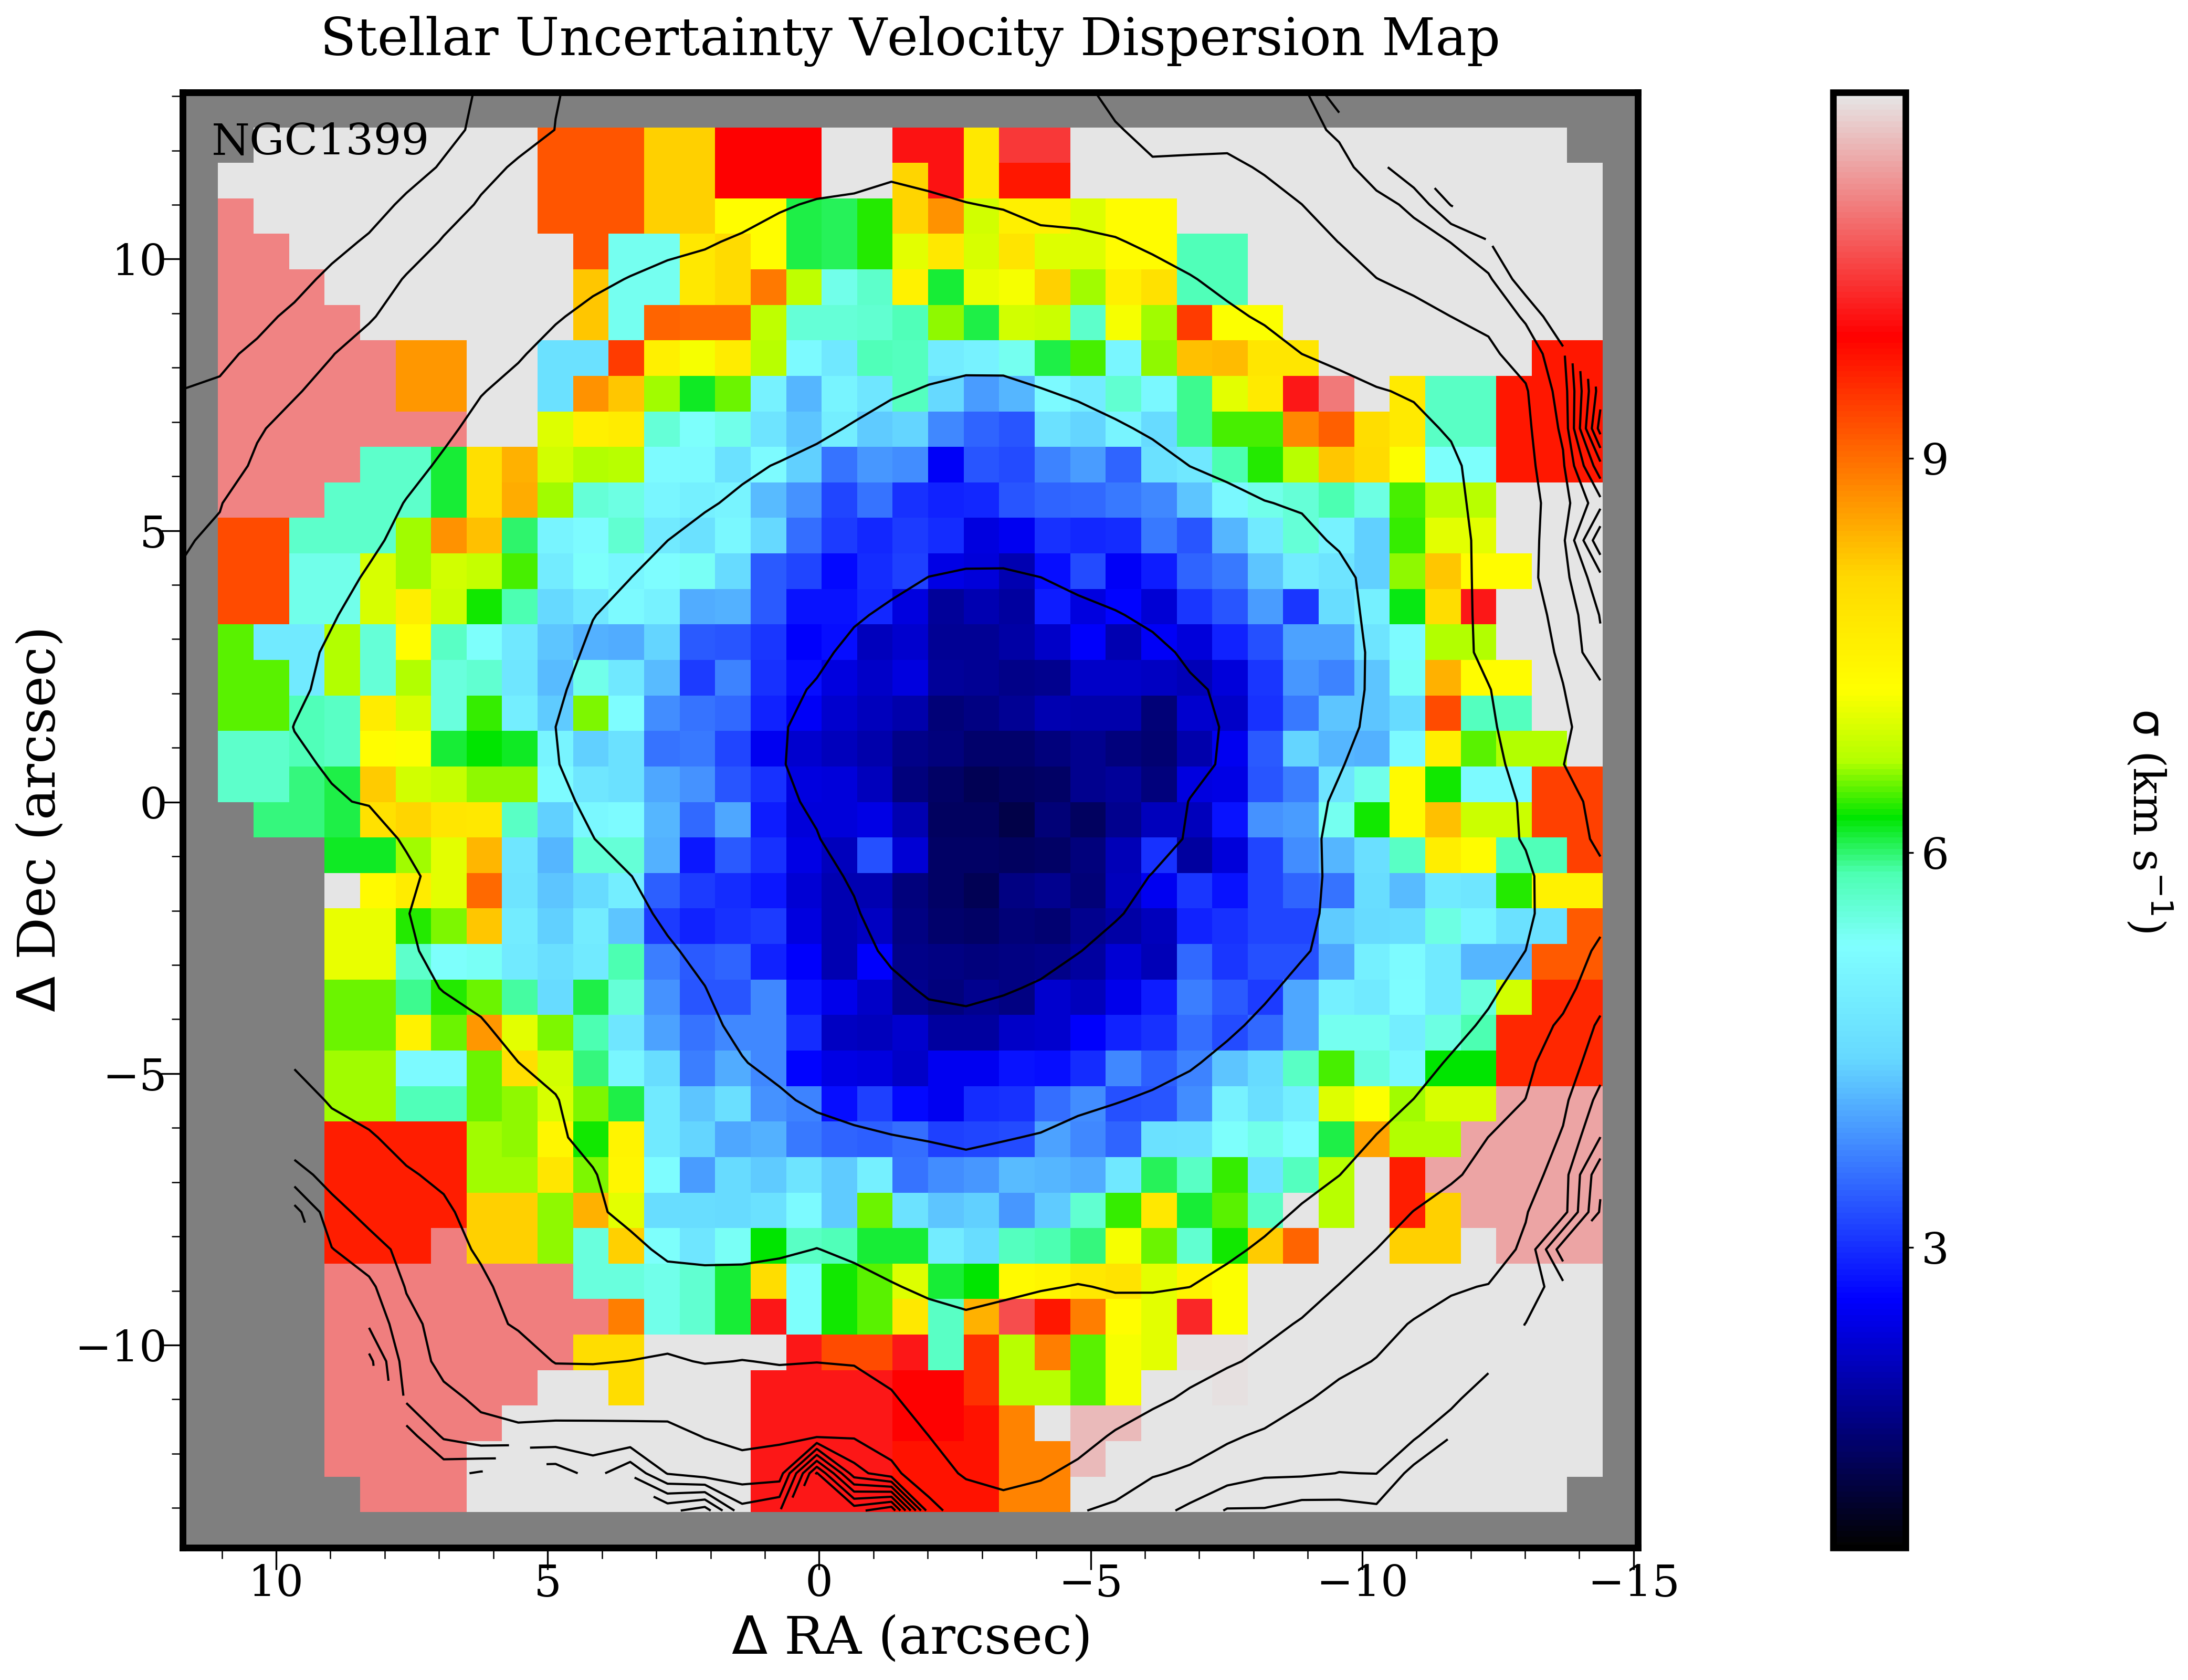
\includegraphics[width=0.245\textwidth]{Vmaps/ngc1399_stellar_sigma_uncert.png}
      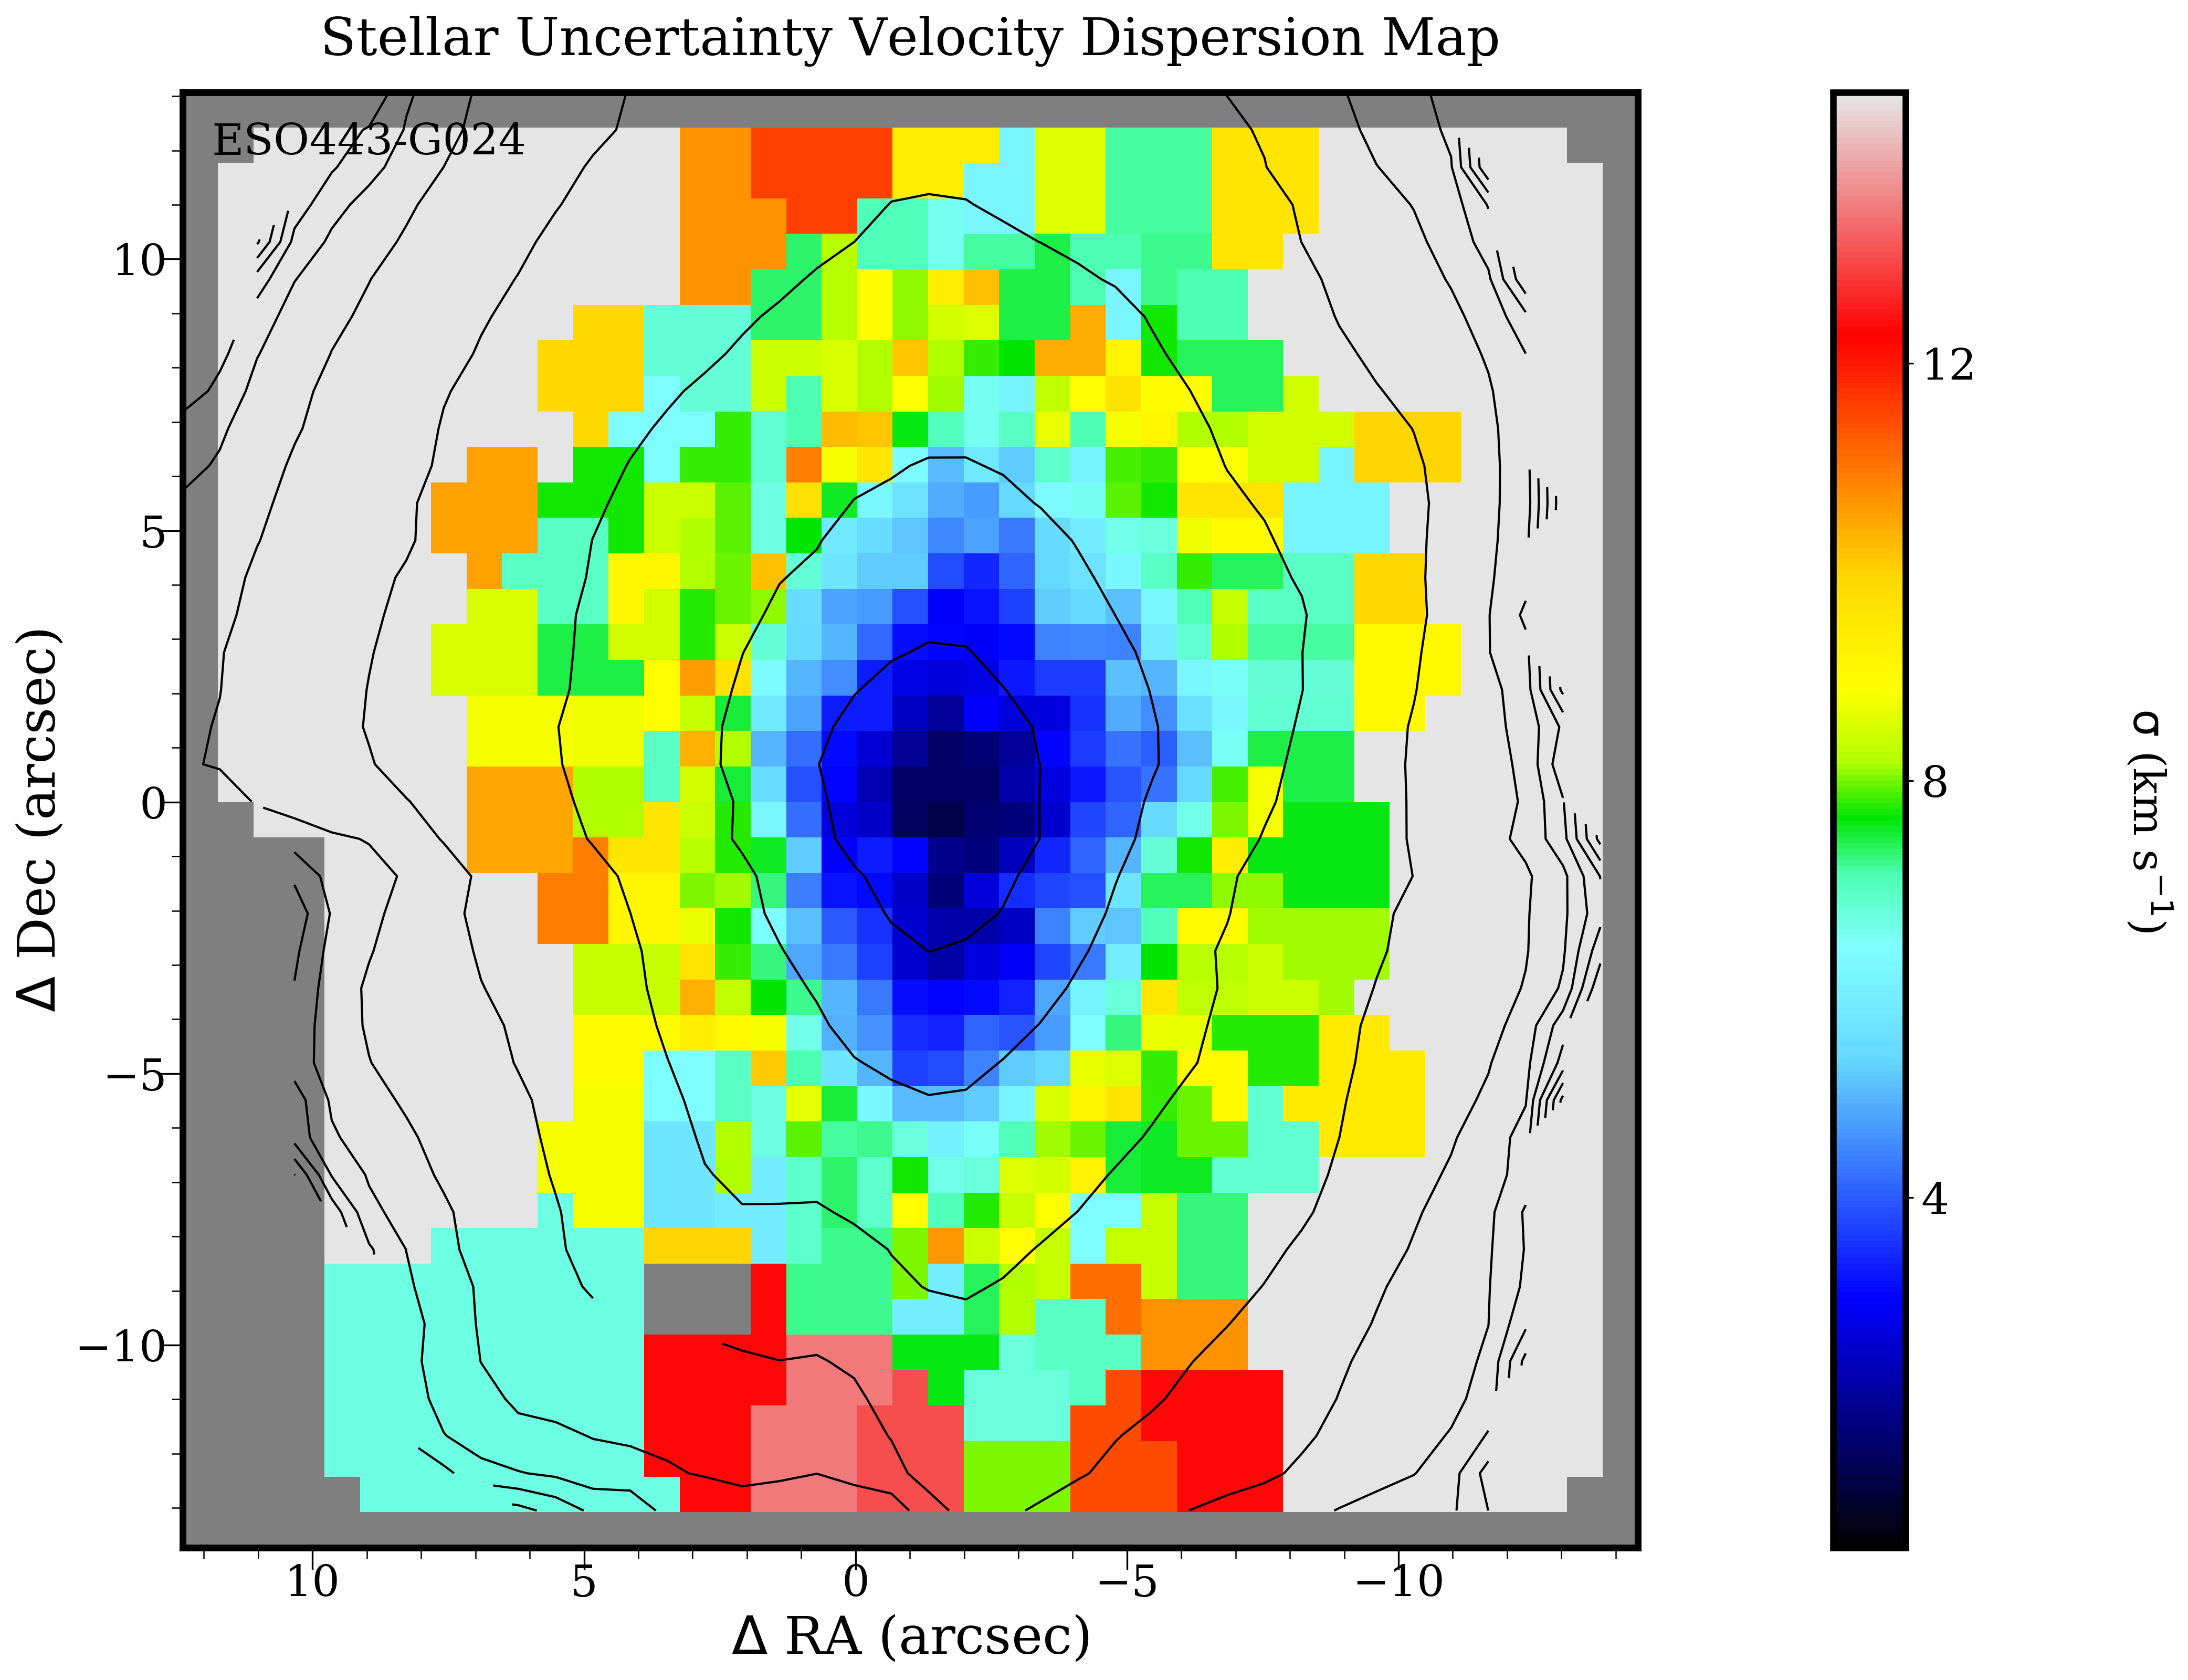
\includegraphics[width=0.245\textwidth]{Vmaps/eso443-g024_stellar_sigma_uncert.png}
      \caption[VIMOS dispersion uncertocity maps]{Uncertainties in the velocity dispersion for each galaxy in the VIMOS sample. Plots are ordered and contour colors are as in figure \ref{fig:Vstellar_img}}
      \label{fig:Vstellar_sigma_uncert}
\end{figure*}






\begin{figure*}
      \centering
      \includegraphics[width=0.245\textwidth]{Mmaps/ic1459_stellar_img.png}
      \includegraphics[width=0.245\textwidth]{Mmaps/ngc1316_stellar_img.png}
      \includegraphics[width=0.245\textwidth]{Mmaps/ic4296_stellar_img.png}
      \includegraphics[width=0.245\textwidth]{Mmaps/ngc1399_stellar_img.png}
      \caption[MUSE images]{Image for each galaxy in the MUSE sample. Plots are ordered roughly in peak stellar velocity with the contours as in figure \ref{fig:Vstellar_img}}
      \label{fig:Mstellar_img}
\end{figure*}

\begin{figure*}
      \centering
      \includegraphics[width=0.245\textwidth]{Mmaps/ic1459_stellar_vel.png}
      \includegraphics[width=0.245\textwidth]{Mmaps/ngc1316_stellar_vel.png}
      \includegraphics[width=0.245\textwidth]{Mmaps/ic4296_stellar_vel.png}
      \includegraphics[width=0.245\textwidth]{Mmaps/ngc1399_stellar_vel.png}
      \caption[MUSE velocity maps]{Velocity for each galaxy in the MUSE sample. Plots are ordered as in figure \ref{fig:Mstellar_img} and contour colors are as in figure \ref{fig:Vstellar_img}}
      \label{fig:stellar_vel}
\end{figure*}

\begin{figure*}
      \centering
      \includegraphics[width=0.245\textwidth]{Mmaps/ic1459_stellar_vel_uncert.png}
      \includegraphics[width=0.245\textwidth]{Mmaps/ngc1316_stellar_vel_uncert.png}
      \includegraphics[width=0.245\textwidth]{Mmaps/ic4296_stellar_vel_uncert.png}
      \includegraphics[width=0.245\textwidth]{Mmaps/ngc1399_stellar_vel_uncert.png}
      \caption[MUSE velocity uncertocity maps]{Uncertainties in the velocity for each galaxy in the MUSE sample. Plots are ordered as in figure \ref{fig:Mstellar_img} and contour colors are as in figure \ref{fig:Vstellar_img}}
      \label{fig:Mstellar_vel_uncert}
\end{figure*}

\begin{figure*}
      \centering
      \includegraphics[width=0.245\textwidth]{Mmaps/ic1459_stellar_sigma.png}
      \includegraphics[width=0.245\textwidth]{Mmaps/ngc1316_stellar_sigma.png}
      \includegraphics[width=0.245\textwidth]{Mmaps/ic4296_stellar_sigma.png}
      \includegraphics[width=0.245\textwidth]{Mmaps/ngc1399_stellar_sigma.png}
      \caption[MUSE velocity dispersion]{Velocity dispersion for each galaxy in the MUSE sample. Plots are ordered as in figure \ref{fig:Mstellar_img} and contour colors are as in figure \ref{fig:Vstellar_img}}
      \label{fig:Mstellar_sigma}
\end{figure*}


\begin{figure*}
      \centering
      \includegraphics[width=0.245\textwidth]{Mmaps/ic1459_stellar_sigma_uncert.png}
      \includegraphics[width=0.245\textwidth]{Mmaps/ngc1316_stellar_sigma_uncert.png}
      \includegraphics[width=0.245\textwidth]{Mmaps/ic4296_stellar_sigma_uncert.png}
      \includegraphics[width=0.245\textwidth]{Mmaps/ngc1399_stellar_sigma_uncert.png}
      \caption[MUSE dispersion uncertocity maps]{Uncertainties in the velocity dispersion for each galaxy in the MUSE sample. Plots are ordered as in figure \ref{fig:Mstellar_img} and contour colors are as in figure \ref{fig:Vstellar_img}}
      \label{fig:Mstellar_sigma_uncert}
\end{figure*}

		Figures \ref{fig:VIMOS_stellar} and \ref{fig:MUSE_stellar} show the stellar LOSVD with associated uncertainties for all VIMOS and MUSE datacubes. 

		The kinematics of the sample are classified according to the Regular-Rotator/Non Regular-Rotator (RR/NRR) regime given in \citet{Krajnovic2011}, Fast/Slow Rotator (FR/SR) regime given in \citet{Cappellari2016} (originally defined by \citet{Emsellem2011}, but later refined by \citet{Cappellari2016}). This classification is shown on the $\lambda_{R_e}$--ellipticity plane in figure \ref{fig:lambdaR_ellip}. Beyond this attempts have been made to use the kinematic features as defined in \citet{Krajnovic2011}, however the quality of the data has meant that many have had to be classified by eye as the artifacts from the VIMOS quadrants confuse any ellipse fitting methods. For VIMOS maps, the classifications are done by eye. These classifications are given in table \ref{tab:classify}. 


		\begin{table}
			\centering
			\caption{Kinematic classifications. Where we have MUSE datacubes, the value and classifications from this are given (since they rely on less extrapolation due to the larger field of view of MUSE), otherwise the values are from the VIMOS maps. Col. 1: Galaxy name, Col. 2: $\lambda_{R_e}$, Col. 3: ellipticity, Col. 4: Misalignment between kinematic position angle and photometric position angle, Col. 5: Fast or Slow rotator, Col. 6: Regular rotator or non-regular rotator, Col. 7: Kinematic features (abbreviations defined in section \ref{sec:ETG}), Col. 8: Kinematic group as defined in section \ref{sec:ETG}}
			\label{tab:classify}
			\begin{tabular}{l r r p{0.7cm} p{0.8cm} p{0.8cm} p{1cm} p{1cm}}
				\hline
				\hline
				Galaxy		& $\lambda_{R_e}$ & $\epsilon$  & $\Gamma_\text{kin}$ (deg) & FR/ SR 	& RR/ NRR 	& Feat. & Group 	\\
				\hline 
				ESO 443-G024 & 0.031 & 0.32 & 55.2 	& FR & NRR & KDC & c \\
				IC 1459 	& 0.174 & 0.24 & 87.9	& FR & NRR & KDC & c \\
				IC 1531 	& 0.100 & 0.11 & 64.4 	& SR & NRR & LV & a \\
				IC 4296		& 0.034 & 0.03 & 83.2 	& SR & NRR & KDC & c \\
				NGC 612 	& 0.519 & 0.58 & 7.3 	& FR & RR & -- & e \\
				NGC 1316 	& 0.100 & 0.39 & 72.1 	& SR & NRR & -- & f \\
				NGC 1399 	& 0.090 & 0.12 & 27.2 	& SR & NRR & LV & a \\
				NGC 3100 	& 0.418 & 0.31 & 19.8 	& FR & RR & -- & e \\
				NGC 3557 	& 0.320 & 0.22 & 7.6 	& FR & RR & -- & e\\
				NGC 7075 	& 0.048 & 0.09 & 20.0 	& SR & NRR & -- & b \\
				PKS 0718-34 & 0.152 & 0.18 & 57.7 	& SR & NRR & KDC? & b\\
				\hline
				\hline
			\end{tabular}
		\end{table}

		% More on the misalignments between kine and phot PA. 


	\subsection{Fast/Slow Rotator fraction}
		\label{subsec:FSfrac}
		Using the combined samples of Atlas3D and MASSIVE, we find that there is no discernible difference between the radio selected Southern Sample and the optically selected ETGs of Atlas3D and MASSIVE, once the differences in mass distribution are taken into account. To do this we find the fraction of slow rotators in each mass bin (using $M_k$ as a proxy), shown in black in the lower panel of figure \ref{fig:SRmassFraction}. We using this and the distribution in mass of the Southern Sample (red in upper panel of \ref{fig:SRmassFraction}) to estimate that we should expect $(64 \pm 6)\%$ of the Southern Sample to be slow rotators. This is consistent with out finding of 56\% slow rotators.

		\begin{figure}
			\centering
			\includegraphics[width=\textwidth]{chapter4/lambda_R_ellipticity.png}
			\caption[$\lambda_{R_e}$ -- ellipticity plane]{The $\lambda_{R_e}$ -- ellipticity plane showing the definition for the fast/slow rotator classes (solid black line). Atlas3D galaxies are shown in black \citep{Emsellem2011} and MASSIVE survey galaxies are shown in gray \citep{Veale2017}. The theoretic limit of disk dominated galaxy is shown (solid magenta) with lines of constant intrinsic angular moment with varying inclination (dashed magenta). VIMOS and MUSE measurements are shown in red and blue respectively. Note: the MASSIVE survey does not classify substructure so the MASSIVE sample is simply shown with filled circles.}
			\label{fig:lambdaR_ellip}
		\end{figure}


		

		\begin{figure}
			\centering
			\includegraphics[width=\textwidth]{chapter4/M_k_binned.png}
			\caption[Mass matching global kinematics]{The mass distributions (upper panel) of the combined Atlas3D and MASSIVE surveys (black) and the Southern Sample (red), as well as the slow rotators fractions within each mass bin (lower panel). The labels display the [number of slow rotators]/[total number of galaxies] in that bin. Note that the black and red have different normalizations in the mass distribution plot: The combined Atlas3D and MASSIVE samples contains 300 galaxies, while the Southern Sample is just 11 radio galaxies.}
			\label{fig:SRmassFraction}
		\end{figure}







\section{Stellar Population}
	\label{sec:pop}

	\subsection{Absorption line strengths}
		\label{subsec:absorption}
		Figures \ref{fig:VIMOS_absorption} and \ref{fig:MUSE_absorption} show the resolved absorption line strengths for the Southern Sample. For the VIMOS cubes, we find G4300, Fe4383, Ca4455, Fe4531, H$_\beta$, Fe5015 and Mg$_b$. For the most distant galaxies, the continuum band for Mg$_b$ is redshifted beyond the range of the VIMOS spectrograph. In these cases, we have avoided unnecessary systematics, by not calculating Mg$_b$. For MUSE cubes, we find H$_\beta$, Fe5015, Mg$_b$, Fe5270, Fe5335, Fe5406, Fe5709, Fe5782, NaD, TiO1 and TiO2. Each index is defined in table \ref{tab:abIndex}. 

		\begin{table}
			\centering
			\caption{The definitions used for each index. Reference abbreviations: Tr98: \citet{Trager1998}.}
			\label{tab:abIndex}
			\begin{tabular}{l c c c c}
				\hline
				\hline
				Index 	& Blue cont. 		& Index band 		& Red cont. 	& Ref. \\
				\hline 
				G4300 	& 4266.375--4282.625 & 4281.375--4316.375 & 4318.875--4335.125 & Tr98 \\
				Fe4383 	& 4359.125--4370.375 & 4369.125--4420.375 & 4442.875--4455.375 & Tr98 \\
				Ca4455 	& 4445.875--4454.625 & 4452.125--4474.625 & 4477.125--4492.125 & Tr98 \\
				Fe4531 	& 4504.250--4514.250 & 4514.250--4559.250 & 4560.500--4579.250 & Tr98 \\
				H$_\beta$ & 4827.875--4847.875 & 4847.875--4876.625 & 4876.625--4891.625 & Tr98 \\
				Fe5015 	& 4946.500--4977.750 & 4977.750--5054.000 & 5054.000--5065.250 & Tr98 \\
				Mg$_b$ 	& 5142.625--5161.375 & 5160.125--5192.625 & 5191.375--5206.375 & Tr98 \\
				Fe5270 	& 5233.150--5248.150 & 5245.650--5285.650 & 5285.650--5318.150 & Tr98 \\
				Fe5335 	& 5304.625--5315.875 & 5312.125--5352.125 & 5353.375--5363.375 & Tr98 \\
				Fe5406 	& 5376.250--5387.500 & 5387.500--5415.000 & 5415.000--5425.000 & Tr98 \\
				Fe5709 	& 5672.875--5696.625 & 5696.625--5720.375 & 5722.875--5736.625 & Tr98 \\
				Fe5782 	& 5765.375--5775.375 & 5776.625--5796.625 & 5797.875--5811.625 & Tr98 \\
				NaD 	& 5860.625--5875.625 & 5876.875--5909.375 & 5922.125--5948.125 & Tr98 \\
				TiO1 	& 5816.625--5849.125 & 5936.625--5994.125 & 6038.625--6103.625 & Tr98 \\
				TiO2 	& 6066.625--6141.625 & 6189.625--6272.125 & 6372.625--6415.125 & Tr98 \\
				\hline
				\hline
			\end{tabular}
		\end{table}

	% \begin{figure*}
	\centering
	\includegraphics[width=0.2\textwidth]{chapter4/Vmaps2/eso443-g024_G4300.png}
	\includegraphics[width=0.2\textwidth]{chapter4/Vmaps2/eso443-g024_G4300_uncert.png}
	\includegraphics[width=0.2\textwidth]{chapter4/Vmaps2/ic1459_G4300.png}
	\includegraphics[width=0.2\textwidth]{chapter4/Vmaps2/ic1459_G4300_uncert.png}
	\\
	\includegraphics[width=0.2\textwidth]{chapter4/Vmaps2/eso443-g024_Fe4383.png}
	\includegraphics[width=0.2\textwidth]{chapter4/Vmaps2/eso443-g024_Fe4383_uncert.png}
	\includegraphics[width=0.2\textwidth]{chapter4/Vmaps2/ic1459_Fe4383.png}
	\includegraphics[width=0.2\textwidth]{chapter4/Vmaps2/ic1459_Fe4383_uncert.png}
	\\
	\includegraphics[width=0.2\textwidth]{chapter4/Vmaps2/eso443-g024_Ca4455.png}
	\includegraphics[width=0.2\textwidth]{chapter4/Vmaps2/eso443-g024_Ca4455_uncert.png}
	\includegraphics[width=0.2\textwidth]{chapter4/Vmaps2/ic1459_Ca4455.png}
	\includegraphics[width=0.2\textwidth]{chapter4/Vmaps2/ic1459_Ca4455_uncert.png}
	\\
	\includegraphics[width=0.2\textwidth]{chapter4/Vmaps2/eso443-g024_Fe4531.png}
	\includegraphics[width=0.2\textwidth]{chapter4/Vmaps2/eso443-g024_Fe4531_uncert.png}
	\includegraphics[width=0.2\textwidth]{chapter4/Vmaps2/ic1459_Fe4531.png}
	\includegraphics[width=0.2\textwidth]{chapter4/Vmaps2/ic1459_Fe4531_uncert.png}
	\\
	\includegraphics[width=0.2\textwidth]{chapter4/Vmaps2/eso443-g024_H_beta.png}
	\includegraphics[width=0.2\textwidth]{chapter4/Vmaps2/eso443-g024_H_beta_uncert.png}
	\includegraphics[width=0.2\textwidth]{chapter4/Vmaps2/ic1459_H_beta.png}
	\includegraphics[width=0.2\textwidth]{chapter4/Vmaps2/ic1459_H_beta_uncert.png}
	\\
	\includegraphics[width=0.2\textwidth]{chapter4/Vmaps2/eso443-g024_Fe5015.png}
	\includegraphics[width=0.2\textwidth]{chapter4/Vmaps2/eso443-g024_Fe5015_uncert.png}
	\includegraphics[width=0.2\textwidth]{chapter4/Vmaps2/ic1459_Fe5015.png}
	\includegraphics[width=0.2\textwidth]{chapter4/Vmaps2/ic1459_Fe5015_uncert.png}
	\\
	\includegraphics[width=0.2\textwidth]{chapter4/Vmaps2/eso443-g024_Mg_b.png}
	\includegraphics[width=0.2\textwidth]{chapter4/Vmaps2/eso443-g024_Mg_b_uncert.png}
	\includegraphics[width=0.2\textwidth]{chapter4/Vmaps2/ic1459_Mg_b.png}
	\includegraphics[width=0.2\textwidth]{chapter4/Vmaps2/ic1459_Mg_b_uncert.png}
	\\
	\caption[VIMOS absorption line strength maps]{VIMOS stellar kinematic maps: From left to right: ESO443-G024, ESO443-G024 uncertianties, IC1459 and IC1459 uncertainties. From top to bottom: G4300, Fe4383, Ca4455, Fe4531, H$_\beta$, Fe5015, Mg$_b$. Plots are as in \ref{fig:VIMOS_stellar}}
	\label{fig:VIMOS_absorption}
\end{figure*}

\begin{figure*}
	\centering
	\includegraphics[width=0.2\textwidth]{chapter4/Vmaps2/ic1531_G4300.png}
	\includegraphics[width=0.2\textwidth]{chapter4/Vmaps2/ic1531_G4300_uncert.png}
	\includegraphics[width=0.2\textwidth]{chapter4/Vmaps2/ic4296_G4300.png}
	\includegraphics[width=0.2\textwidth]{chapter4/Vmaps2/ic4296_G4300_uncert.png}
	\\
	\includegraphics[width=0.2\textwidth]{chapter4/Vmaps2/ic1531_Fe4383.png}
	\includegraphics[width=0.2\textwidth]{chapter4/Vmaps2/ic1531_Fe4383_uncert.png}
	\includegraphics[width=0.2\textwidth]{chapter4/Vmaps2/ic4296_Fe4383.png}
	\includegraphics[width=0.2\textwidth]{chapter4/Vmaps2/ic4296_Fe4383_uncert.png}
	\\
	\includegraphics[width=0.2\textwidth]{chapter4/Vmaps2/ic1531_Ca4455.png}
	\includegraphics[width=0.2\textwidth]{chapter4/Vmaps2/ic1531_Ca4455_uncert.png}
	\includegraphics[width=0.2\textwidth]{chapter4/Vmaps2/ic4296_Ca4455.png}
	\includegraphics[width=0.2\textwidth]{chapter4/Vmaps2/ic4296_Ca4455_uncert.png}
	\\
	\includegraphics[width=0.2\textwidth]{chapter4/Vmaps2/ic1531_Fe4531.png}
	\includegraphics[width=0.2\textwidth]{chapter4/Vmaps2/ic1531_Fe4531_uncert.png}
	\includegraphics[width=0.2\textwidth]{chapter4/Vmaps2/ic4296_Fe4531.png}
	\includegraphics[width=0.2\textwidth]{chapter4/Vmaps2/ic4296_Fe4531_uncert.png}
	\\
	\includegraphics[width=0.2\textwidth]{chapter4/Vmaps2/ic1531_H_beta.png}
	\includegraphics[width=0.2\textwidth]{chapter4/Vmaps2/ic1531_H_beta_uncert.png}
	\includegraphics[width=0.2\textwidth]{chapter4/Vmaps2/ic4296_H_beta.png}
	\includegraphics[width=0.2\textwidth]{chapter4/Vmaps2/ic4296_H_beta_uncert.png}
	\\
	\includegraphics[width=0.2\textwidth]{chapter4/Vmaps2/ic1531_Fe5015.png}
	\includegraphics[width=0.2\textwidth]{chapter4/Vmaps2/ic1531_Fe5015_uncert.png}
	\includegraphics[width=0.2\textwidth]{chapter4/Vmaps2/ic4296_Fe5015.png}
	\includegraphics[width=0.2\textwidth]{chapter4/Vmaps2/ic4296_Fe5015_uncert.png}
	\\
	\includegraphics[width=0.2\textwidth]{chapter4/Vmaps2/ic1531_Mg_b.png}
	\includegraphics[width=0.2\textwidth]{chapter4/Vmaps2/ic1531_Mg_b_uncert.png}
	\includegraphics[width=0.2\textwidth]{chapter4/Vmaps2/ic4296_Mg_b.png}
	\includegraphics[width=0.2\textwidth]{chapter4/Vmaps2/ic4296_Mg_b_uncert.png}
	\\
	\contcaption{continued for ESO443-G024 and IC1459.}
\end{figure*}

\begin{figure*}
	\centering
	\includegraphics[width=0.2\textwidth]{chapter4/Vmaps2/ngc0612_G4300.png}
	\includegraphics[width=0.2\textwidth]{chapter4/Vmaps2/ngc0612_G4300_uncert.png}
	\includegraphics[width=0.2\textwidth]{chapter4/Vmaps2/ngc1399_G4300.png}
	\includegraphics[width=0.2\textwidth]{chapter4/Vmaps2/ngc1399_G4300_uncert.png}
	\\
	\includegraphics[width=0.2\textwidth]{chapter4/Vmaps2/ngc0612_Fe4383.png}
	\includegraphics[width=0.2\textwidth]{chapter4/Vmaps2/ngc0612_Fe4383_uncert.png}
	\includegraphics[width=0.2\textwidth]{chapter4/Vmaps2/ngc1399_Fe4383.png}
	\includegraphics[width=0.2\textwidth]{chapter4/Vmaps2/ngc1399_Fe4383_uncert.png}
	\\
	\includegraphics[width=0.2\textwidth]{chapter4/Vmaps2/ngc0612_Ca4455.png}
	\includegraphics[width=0.2\textwidth]{chapter4/Vmaps2/ngc0612_Ca4455_uncert.png}
	\includegraphics[width=0.2\textwidth]{chapter4/Vmaps2/ngc1399_Ca4455.png}
	\includegraphics[width=0.2\textwidth]{chapter4/Vmaps2/ngc1399_Ca4455_uncert.png}
	\\
	\includegraphics[width=0.2\textwidth]{chapter4/Vmaps2/ngc0612_Fe4531.png}
	\includegraphics[width=0.2\textwidth]{chapter4/Vmaps2/ngc0612_Fe4531_uncert.png}
	\includegraphics[width=0.2\textwidth]{chapter4/Vmaps2/ngc1399_Fe4531.png}
	\includegraphics[width=0.2\textwidth]{chapter4/Vmaps2/ngc1399_Fe4531_uncert.png}
	\\
	\includegraphics[width=0.2\textwidth]{chapter4/Vmaps2/ngc0612_H_beta.png}
	\includegraphics[width=0.2\textwidth]{chapter4/Vmaps2/ngc0612_H_beta_uncert.png}
	\includegraphics[width=0.2\textwidth]{chapter4/Vmaps2/ngc1399_H_beta.png}
	\includegraphics[width=0.2\textwidth]{chapter4/Vmaps2/ngc1399_H_beta_uncert.png}
	\\
	\includegraphics[width=0.2\textwidth]{chapter4/Vmaps2/ngc0612_Fe5015.png}
	\includegraphics[width=0.2\textwidth]{chapter4/Vmaps2/ngc0612_Fe5015_uncert.png}
	\includegraphics[width=0.2\textwidth]{chapter4/Vmaps2/ngc1399_Fe5015.png}
	\includegraphics[width=0.2\textwidth]{chapter4/Vmaps2/ngc1399_Fe5015_uncert.png}
	\\
	\includegraphics[width=0.2\textwidth]{chapter4/Vmaps2/ngc0612_Mg_b.png}
	\includegraphics[width=0.2\textwidth]{chapter4/Vmaps2/ngc0612_Mg_b_uncert.png}
	\includegraphics[width=0.2\textwidth]{chapter4/Vmaps2/ngc1399_Mg_b.png}
	\includegraphics[width=0.2\textwidth]{chapter4/Vmaps2/ngc1399_Mg_b_uncert.png}
	\\
	\contcaption{continued for ESO443-G024 and IC1459.}
\end{figure*}

\begin{figure*}
	\centering
	\includegraphics[width=0.2\textwidth]{chapter4/Vmaps2/ngc3100_G4300.png}
	\includegraphics[width=0.2\textwidth]{chapter4/Vmaps2/ngc3100_G4300_uncert.png}
	\includegraphics[width=0.2\textwidth]{chapter4/Vmaps2/ngc3557_G4300.png}
	\includegraphics[width=0.2\textwidth]{chapter4/Vmaps2/ngc3557_G4300_uncert.png}
	\\
	\includegraphics[width=0.2\textwidth]{chapter4/Vmaps2/ngc3100_Fe4383.png}
	\includegraphics[width=0.2\textwidth]{chapter4/Vmaps2/ngc3100_Fe4383_uncert.png}
	\includegraphics[width=0.2\textwidth]{chapter4/Vmaps2/ngc3557_Fe4383.png}
	\includegraphics[width=0.2\textwidth]{chapter4/Vmaps2/ngc3557_Fe4383_uncert.png}
	\\
	\includegraphics[width=0.2\textwidth]{chapter4/Vmaps2/ngc3100_Ca4455.png}
	\includegraphics[width=0.2\textwidth]{chapter4/Vmaps2/ngc3100_Ca4455_uncert.png}
	\includegraphics[width=0.2\textwidth]{chapter4/Vmaps2/ngc3557_Ca4455.png}
	\includegraphics[width=0.2\textwidth]{chapter4/Vmaps2/ngc3557_Ca4455_uncert.png}
	\\
	\includegraphics[width=0.2\textwidth]{chapter4/Vmaps2/ngc3100_Fe4531.png}
	\includegraphics[width=0.2\textwidth]{chapter4/Vmaps2/ngc3100_Fe4531_uncert.png}
	\includegraphics[width=0.2\textwidth]{chapter4/Vmaps2/ngc3557_Fe4531.png}
	\includegraphics[width=0.2\textwidth]{chapter4/Vmaps2/ngc3557_Fe4531_uncert.png}
	\\
	\includegraphics[width=0.2\textwidth]{chapter4/Vmaps2/ngc3100_H_beta.png}
	\includegraphics[width=0.2\textwidth]{chapter4/Vmaps2/ngc3100_H_beta_uncert.png}
	\includegraphics[width=0.2\textwidth]{chapter4/Vmaps2/ngc3557_H_beta.png}
	\includegraphics[width=0.2\textwidth]{chapter4/Vmaps2/ngc3557_H_beta_uncert.png}
	\\
	\includegraphics[width=0.2\textwidth]{chapter4/Vmaps2/ngc3100_Fe5015.png}
	\includegraphics[width=0.2\textwidth]{chapter4/Vmaps2/ngc3100_Fe5015_uncert.png}
	\includegraphics[width=0.2\textwidth]{chapter4/Vmaps2/ngc3557_Fe5015.png}
	\includegraphics[width=0.2\textwidth]{chapter4/Vmaps2/ngc3557_Fe5015_uncert.png}
	\\
	\includegraphics[width=0.2\textwidth]{chapter4/Vmaps2/ngc3100_Mg_b.png}
	\includegraphics[width=0.2\textwidth]{chapter4/Vmaps2/ngc3100_Mg_b_uncert.png}
	\includegraphics[width=0.2\textwidth]{chapter4/Vmaps2/ngc3557_Mg_b.png}
	\includegraphics[width=0.2\textwidth]{chapter4/Vmaps2/ngc3557_Mg_b_uncert.png}
	\\
	\contcaption{continued for ESO443-G024 and IC1459.}
\end{figure*}

\begin{figure*}
	\centering
	\includegraphics[width=0.2\textwidth]{chapter4/Vmaps2/ngc7075_G4300.png}
	\includegraphics[width=0.2\textwidth]{chapter4/Vmaps2/ngc7075_G4300_uncert.png}
	\includegraphics[width=0.2\textwidth]{chapter4/Vmaps2/pks0718-34_G4300.png}
	\includegraphics[width=0.2\textwidth]{chapter4/Vmaps2/pks0718-34_G4300_uncert.png}
	\\
	\includegraphics[width=0.2\textwidth]{chapter4/Vmaps2/ngc7075_Fe4383.png}
	\includegraphics[width=0.2\textwidth]{chapter4/Vmaps2/ngc7075_Fe4383_uncert.png}
	\includegraphics[width=0.2\textwidth]{chapter4/Vmaps2/pks0718-34_Fe4383.png}
	\includegraphics[width=0.2\textwidth]{chapter4/Vmaps2/pks0718-34_Fe4383_uncert.png}
	\\
	\includegraphics[width=0.2\textwidth]{chapter4/Vmaps2/ngc7075_Ca4455.png}
	\includegraphics[width=0.2\textwidth]{chapter4/Vmaps2/ngc7075_Ca4455_uncert.png}
	\includegraphics[width=0.2\textwidth]{chapter4/Vmaps2/pks0718-34_Ca4455.png}
	\includegraphics[width=0.2\textwidth]{chapter4/Vmaps2/pks0718-34_Ca4455_uncert.png}
	\\
	\includegraphics[width=0.2\textwidth]{chapter4/Vmaps2/ngc7075_Fe4531.png}
	\includegraphics[width=0.2\textwidth]{chapter4/Vmaps2/ngc7075_Fe4531_uncert.png}
	\includegraphics[width=0.2\textwidth]{chapter4/Vmaps2/pks0718-34_Fe4531.png}
	\includegraphics[width=0.2\textwidth]{chapter4/Vmaps2/pks0718-34_Fe4531_uncert.png}
	\\
	\includegraphics[width=0.2\textwidth]{chapter4/Vmaps2/ngc7075_H_beta.png}
	\includegraphics[width=0.2\textwidth]{chapter4/Vmaps2/ngc7075_H_beta_uncert.png}
	\includegraphics[width=0.2\textwidth]{chapter4/Vmaps2/pks0718-34_H_beta.png}
	\includegraphics[width=0.2\textwidth]{chapter4/Vmaps2/pks0718-34_H_beta_uncert.png}
	\\
	\includegraphics[width=0.2\textwidth]{chapter4/Vmaps2/ngc7075_Fe5015.png}
	\includegraphics[width=0.2\textwidth]{chapter4/Vmaps2/ngc7075_Fe5015_uncert.png}
	\includegraphics[width=0.2\textwidth]{chapter4/Vmaps2/pks0718-34_Fe5015.png}
	\includegraphics[width=0.2\textwidth]{chapter4/Vmaps2/pks0718-34_Fe5015_uncert.png}
	\\
	\includegraphics[width=0.2\textwidth]{chapter4/Vmaps2/ngc7075_Mg_b.png}
	\includegraphics[width=0.2\textwidth]{chapter4/Vmaps2/ngc7075_Mg_b_uncert.png}
	\includegraphics[width=0.2\textwidth]{chapter4/Vmaps2/pks0718-34_Mg_b.png}
	\includegraphics[width=0.2\textwidth]{chapter4/Vmaps2/pks0718-34_Mg_b_uncert.png}
	\\
	\contcaption{continued for ESO443-G024 and IC1459.}
\end{figure*}


\begin{figure*}
	\centering
	\includegraphics[width=0.2\textwidth]{chapter4/Mmaps2/ic1459_H_beta.png}
	\includegraphics[width=0.2\textwidth]{chapter4/Mmaps2/ic1459_H_beta_uncert.png}
	\includegraphics[width=0.2\textwidth]{chapter4/Mmaps2/ic4296_H_beta.png}
	\includegraphics[width=0.2\textwidth]{chapter4/Mmaps2/ic4296_H_beta_uncert.png}
	\\
	\includegraphics[width=0.2\textwidth]{chapter4/Mmaps2/ic1459_Fe5015.png}
	\includegraphics[width=0.2\textwidth]{chapter4/Mmaps2/ic1459_Fe5015_uncert.png}
	\includegraphics[width=0.2\textwidth]{chapter4/Mmaps2/ic4296_Fe5015.png}
	\includegraphics[width=0.2\textwidth]{chapter4/Mmaps2/ic4296_Fe5015_uncert.png}
	\\
	\includegraphics[width=0.2\textwidth]{chapter4/Mmaps2/ic1459_Mg_b.png}
	\includegraphics[width=0.2\textwidth]{chapter4/Mmaps2/ic1459_Mg_b_uncert.png}
	\includegraphics[width=0.2\textwidth]{chapter4/Mmaps2/ic4296_Mg_b.png}
	\includegraphics[width=0.2\textwidth]{chapter4/Mmaps2/ic4296_Mg_b_uncert.png}
	\\
	\includegraphics[width=0.2\textwidth]{chapter4/Mmaps2/ic1459_Fe5270.png}
	\includegraphics[width=0.2\textwidth]{chapter4/Mmaps2/ic1459_Fe5270_uncert.png}
	\includegraphics[width=0.2\textwidth]{chapter4/Mmaps2/ic4296_Fe5270.png}
	\includegraphics[width=0.2\textwidth]{chapter4/Mmaps2/ic4296_Fe5270_uncert.png}
	\\
	\includegraphics[width=0.2\textwidth]{chapter4/Mmaps2/ic1459_Fe5335.png}
	\includegraphics[width=0.2\textwidth]{chapter4/Mmaps2/ic1459_Fe5335_uncert.png}
	\includegraphics[width=0.2\textwidth]{chapter4/Mmaps2/ic4296_Fe5335.png}
	\includegraphics[width=0.2\textwidth]{chapter4/Mmaps2/ic4296_Fe5335_uncert.png}
	\\
	\includegraphics[width=0.2\textwidth]{chapter4/Mmaps2/ic1459_Fe5406.png}
	\includegraphics[width=0.2\textwidth]{chapter4/Mmaps2/ic1459_Fe5406_uncert.png}
	\includegraphics[width=0.2\textwidth]{chapter4/Mmaps2/ic4296_Fe5406.png}
	\includegraphics[width=0.2\textwidth]{chapter4/Mmaps2/ic4296_Fe5406_uncert.png}
	\\
	\includegraphics[width=0.2\textwidth]{chapter4/Mmaps2/ic1459_Fe5709.png}
	\includegraphics[width=0.2\textwidth]{chapter4/Mmaps2/ic1459_Fe5709_uncert.png}
	\includegraphics[width=0.2\textwidth]{chapter4/Mmaps2/ic4296_Fe5709.png}
	\includegraphics[width=0.2\textwidth]{chapter4/Mmaps2/ic4296_Fe5709_uncert.png}
	\\
	\caption[MUSE absorption line strength maps]{MUSE stellar kinematic maps: From left to right: IC1459, IC1459 uncertianties, IC4296 and IC4296 uncertainties. From top to bottom: H$_\beta$, Fe5015, Mg$_b$, Fe5270, Fe5335, Fe5406, Fe5709. Plots are as in \ref{fig:VIMOS_stellar}}
	\label{fig:MUSE_stellar1}
\end{figure*}

\begin{figure*}
	\centering
	\includegraphics[width=0.2\textwidth]{chapter4/M2maps2/ic1459_Fe5782.png}
	\includegraphics[width=0.2\textwidth]{chapter4/M2maps2/ic1459_Fe5782_uncert.png}
	\includegraphics[width=0.2\textwidth]{chapter4/M2maps2/ic4296_Fe5782.png}
	\includegraphics[width=0.2\textwidth]{chapter4/M2maps2/ic4296_Fe5782_uncert.png}
	\\
	\includegraphics[width=0.2\textwidth]{chapter4/M2maps2/ic1459_NaD.png}
	\includegraphics[width=0.2\textwidth]{chapter4/M2maps2/ic1459_NaD_uncert.png}
	\includegraphics[width=0.2\textwidth]{chapter4/M2maps2/ic4296_NaD.png}
	\includegraphics[width=0.2\textwidth]{chapter4/M2maps2/ic4296_NaD_uncert.png}
	\\
	\includegraphics[width=0.2\textwidth]{chapter4/M2maps2/ic1459_TiO1.png}
	\includegraphics[width=0.2\textwidth]{chapter4/M2maps2/ic1459_TiO1_uncert.png}
	\includegraphics[width=0.2\textwidth]{chapter4/M2maps2/ic4296_TiO1.png}
	\includegraphics[width=0.2\textwidth]{chapter4/M2maps2/ic4296_TiO1_uncert.png}
	\\
	\includegraphics[width=0.2\textwidth]{chapter4/M2maps2/ic1459_TiO2.png}
	\includegraphics[width=0.2\textwidth]{chapter4/M2maps2/ic1459_TiO2_uncert.png}
	\includegraphics[width=0.2\textwidth]{chapter4/M2maps2/ic4296_TiO2.png}
	\includegraphics[width=0.2\textwidth]{chapter4/M2maps2/ic4296_TiO2_uncert.png}
	\\
	\contcaption{continued: From top to bottom: Fe5782, NaD, TiO1, TiO2. Plots are as in \ref{fig:VIMOS_stellar}}
	\label{fig:MUSE_stellar1}
\end{figure*}

\begin{figure*}
	\centering
	\includegraphics[width=0.2\textwidth]{chapter4/Mmaps2/ngc1316_H_beta.png}
	\includegraphics[width=0.2\textwidth]{chapter4/Mmaps2/ngc1316_H_beta_uncert.png}
	\includegraphics[width=0.2\textwidth]{chapter4/Mmaps2/ngc1399_H_beta.png}
	\includegraphics[width=0.2\textwidth]{chapter4/Mmaps2/ngc1399_H_beta_uncert.png}
	\\
	\includegraphics[width=0.2\textwidth]{chapter4/Mmaps2/ngc1316_Fe5015.png}
	\includegraphics[width=0.2\textwidth]{chapter4/Mmaps2/ngc1316_Fe5015_uncert.png}
	\includegraphics[width=0.2\textwidth]{chapter4/Mmaps2/ngc1399_Fe5015.png}
	\includegraphics[width=0.2\textwidth]{chapter4/Mmaps2/ngc1399_Fe5015_uncert.png}
	\\
	\includegraphics[width=0.2\textwidth]{chapter4/Mmaps2/ngc1316_Mg_b.png}
	\includegraphics[width=0.2\textwidth]{chapter4/Mmaps2/ngc1316_Mg_b_uncert.png}
	\includegraphics[width=0.2\textwidth]{chapter4/Mmaps2/ngc1399_Mg_b.png}
	\includegraphics[width=0.2\textwidth]{chapter4/Mmaps2/ngc1399_Mg_b_uncert.png}
	\\
	\includegraphics[width=0.2\textwidth]{chapter4/Mmaps2/ngc1316_Fe5270.png}
	\includegraphics[width=0.2\textwidth]{chapter4/Mmaps2/ngc1316_Fe5270_uncert.png}
	\includegraphics[width=0.2\textwidth]{chapter4/Mmaps2/ngc1399_Fe5270.png}
	\includegraphics[width=0.2\textwidth]{chapter4/Mmaps2/ngc1399_Fe5270_uncert.png}
	\\
	\includegraphics[width=0.2\textwidth]{chapter4/Mmaps2/ngc1316_Fe5335.png}
	\includegraphics[width=0.2\textwidth]{chapter4/Mmaps2/ngc1316_Fe5335_uncert.png}
	\includegraphics[width=0.2\textwidth]{chapter4/Mmaps2/ngc1399_Fe5335.png}
	\includegraphics[width=0.2\textwidth]{chapter4/Mmaps2/ngc1399_Fe5335_uncert.png}
	\\
	\includegraphics[width=0.2\textwidth]{chapter4/Mmaps2/ngc1316_Fe5406.png}
	\includegraphics[width=0.2\textwidth]{chapter4/Mmaps2/ngc1316_Fe5406_uncert.png}
	\includegraphics[width=0.2\textwidth]{chapter4/Mmaps2/ngc1399_Fe5406.png}
	\includegraphics[width=0.2\textwidth]{chapter4/Mmaps2/ngc1399_Fe5406_uncert.png}
	\\
	\includegraphics[width=0.2\textwidth]{chapter4/Mmaps2/ngc1316_Fe5709.png}
	\includegraphics[width=0.2\textwidth]{chapter4/Mmaps2/ngc1316_Fe5709_uncert.png}
	\includegraphics[width=0.2\textwidth]{chapter4/Mmaps2/ngc1399_Fe5709.png}
	\includegraphics[width=0.2\textwidth]{chapter4/Mmaps2/ngc1399_Fe5709_uncert.png}
	\\
	\contcaption{continued for NGC1316 and NGC1399.}
	\label{fig:MUSE_stellar2}
\end{figure*}

\begin{figure*}
	\centering
	\includegraphics[width=0.2\textwidth]{chapter4/M2maps2/ngc1316_Fe5782.png}
	\includegraphics[width=0.2\textwidth]{chapter4/M2maps2/ngc1316_Fe5782_uncert.png}
	\includegraphics[width=0.2\textwidth]{chapter4/M2maps2/ngc1399_Fe5782.png}
	\includegraphics[width=0.2\textwidth]{chapter4/M2maps2/ngc1399_Fe5782_uncert.png}
	\\
	\includegraphics[width=0.2\textwidth]{chapter4/M2maps2/ngc1316_NaD.png}
	\includegraphics[width=0.2\textwidth]{chapter4/M2maps2/ngc1316_NaD_uncert.png}
	\includegraphics[width=0.2\textwidth]{chapter4/M2maps2/ngc1399_NaD.png}
	\includegraphics[width=0.2\textwidth]{chapter4/M2maps2/ngc1399_NaD_uncert.png}
	\\
	\includegraphics[width=0.2\textwidth]{chapter4/M2maps2/ngc1316_TiO1.png}
	\includegraphics[width=0.2\textwidth]{chapter4/M2maps2/ngc1316_TiO1_uncert.png}
	\includegraphics[width=0.2\textwidth]{chapter4/M2maps2/ngc1399_TiO1.png}
	\includegraphics[width=0.2\textwidth]{chapter4/M2maps2/ngc1399_TiO1_uncert.png}
	\\
	\includegraphics[width=0.2\textwidth]{chapter4/M2maps2/ngc1316_TiO2.png}
	\includegraphics[width=0.2\textwidth]{chapter4/M2maps2/ngc1316_TiO2_uncert.png}
	\includegraphics[width=0.2\textwidth]{chapter4/M2maps2/ngc1399_TiO2.png}
	\includegraphics[width=0.2\textwidth]{chapter4/M2maps2/ngc1399_TiO2_uncert.png}
	\\
	\contcaption{continued for NGC1316 and NGC1399.}
	\label{fig:MUSE_stellar2}
\end{figure*}

	Comparisons to the literature is made difficult by the inhomogeneous nature of corrections applied: such as accounting for H$_\beta$ emission or velocity dispersion. We use Line Index System (LIS) by \citet{Vazdekis2010} instead of the popular LICK/IDS system \citep{Faber1985, Worthey1994} as LICK/IDS is based on non-flux calibrated spectra from the IDS and Cassegrain spectrograph on the Shane telescope (Lick Observatory) which has a relatively low and wavelength dependent resolution. In order to make calibrate measurements from other instruments it is necessary to perform empirical corrections to correct for the uncalibrated continuum. This requires observing standard stars with the same instrumental set up as the main observations in order to make comparisons to the measurements from the IDS spectrograph. Since this was not requested as part of the observing strategy with VIMOS we were not able to do this: a later proposal would not have worked since VIMOS was substantially upgraded in the intervening time period. Further more, we believe that this system has had its time and the community should be making a concerted effort to move away from it, due to the low resolution and poor data quality on which it is based. However, there is a lack of non-LICK/IDS system measurements: we used the empirical functions provided by \citet{Vazdekis2010} to translate between LICK/IDS and LIS systems\footnote{The transformation from LICK/IDS to the LIS system is available at http://www.iac.es/proyecto/miles/pages/line-index-system-lis/transformations.php.}. 


	Finally, we noticed that only the H$_\beta$ emission line is corrected for in some of the literature, despite [OIII] often being the strongest emission line for ETGs. This effects the reliability of the Fe5015 and Mb$_b$ absorption indices as the [OIII] and [NI] doublets fall within them respectively. They vary as to whether they fall within the index band or the continuum bands and the effect depends on the relative difference in the kinematics for the stars (which result in the absorption features) and the ISM (which results in the emission lines). Other papers correct for only H$_\beta$ and [OIII]. In order to make accurate comparisons to the literature we mimic the corrections in the relevant paper for the comparison only, while removing all emission lines (given in table \ref{}) for our quoted measurements and maps. Table \ref{tab:litAbsorption} sums up our comparisons to the literature. Here we note that in the case of comparisons to \citet{Rampazzo2005}, G4300 has a very large offset. We suggest that this index is extremely sensitive to the velocity dispersion due to the steep nature of the pseudo-continuum: a difference of $30 \mathrm{km \, s^{-1}}$ can effect the corrected index value by $\sim 2$\AA. For the comparison to \citet{Vazdekis2010}, we analyzed the SAURON data set\footnote{SARUON data is available at: http://www.strw.leidenuniv.nl/sauron/} \citep{Emsellem2004} using the same pipeline we have developed for our sample. 

	% Could use another paper to compare to: Orgando? 
	\begin{table}
		\centering
		\caption{Comparisons to the literature. Comparisons to \citet{Rampazzo2005} are sampled at 7 radial apertures for each galaxy: 1.5, 2.5 and 10.0 arcsec and R$_e$/10, R$_e$/8, R$_e$/4 and R$_e$/2. Offset is the mean difference between our measurements and that of the literature, while Dispersion is the standard deviation of the difference.}
		\label{tab:litAbsorption}
		\begin{tabular}{l r r r}
			\hline
			\hline
			Index 		& N$_{gals}$ & Offset 	& Dispersion \\
						& 			& $\AA$		& $\AA$ \\
			\hline
			\multicolumn{4}{c}{\citet{Vazdekis2010} (SAURON)} \\
			\hline
			H$_\beta$ 	& 46		& -0.02		& 0.25	\\
			Fe5015		& 46		& 0.66		& 0.34	\\
			Mg$_b$ 		& 46		& 0.06		& 0.33	\\
			\hline
			\multicolumn{4}{c}{\citet{Rampazzo2005} (VIMOS)} \\
			\hline
			G4300 		& 3 		& 2.29		& 0.11	\\
			Fe4383 		& 3 		& 0.39		& 0.23	\\
			Ca4455 		& 3 		& -0.19		& 0.09	\\
			Fe4531 		& 3 		& 0.16		& 0.26	\\
			H$_\beta$ 	& 3 		& 0.17		& 0.12	\\
			Fe5015 		& 3 		& -0.73		& 0.48	\\
			Mg$_b$ 		& 3 		& -0.43		& 0.17	\\
			\hline
			\multicolumn{4}{c}{\citet{Rampazzo2005} (MUSE)} \\
			\hline
			H$_\beta$ 	& 2 		& -0.28		& 0.17	\\ 
			Fe5015 		& 2 		& 0.87		& 0.34	\\ 
			Mg$_b$ 		& 2 		& 0.31		& 0.14	\\
			Fe5270 		& 2 		& -0.11		& 0.15	\\
			Fe5335 		& 2 		& 0.08		& 0.15	\\
			Fe5406 		& 2 		& 0.16		& 0.07	\\
			Fe5709 		& 2 		& 0.11		& 0.10	\\
			Fe5782 		& 2 		& -0.03		& 0.11	\\
			NaD 		& 2 		& 0.90		& 0.41	\\
			TiO1 (mag)	& 2 		& -0.004	& 0.003	\\
			TiO2 (mag)	& 2 		& -0.011	& 0.007	\\
			\hline
			\multicolumn{4}{c}{\citet{Ogando2008} (VIMOS)} \\
			\hline
			H$_\beta$ 	& 6 		& 		& 	\\
			Fe5015 		& 6 		& 		& 	\\
			Mg$_b$ 		& 6 		& 		& 	\\
			\hline
			\multicolumn{4}{c}{\citet{Ogando2008} (MUSE)} \\
			\hline
			H$_\beta$ 	& 3 		& 		& 	\\ 
			Fe5015 		& 3 		& 		& 	\\ 
			Mg$_b$ 		& 3 		& 		& 	\\
			Fe5270 		& 3 		& 		& 	\\
			Fe5335 		& 3 		& 		& 	\\
			Fe5406 		& 3 		& 		& 	\\
			Fe5709 		& 3 		& 		& 	\\
			NaD 		& 3 		& 		& 	\\
			%[OIII]5007	& 3 		& 		& 	\\
			\hline
		\end{tabular}
	\end{table}

	% \subsection{Gradients in absorption line strengths}
	% 	\label{subsec:absorptionGrad}


	\subsection{Most-likely stellar population model}
		\label{subsec:ssp}

		% Need to go into more detail about the TMJ models
		% What the pecularities of the SSPs they used.
		% Which IMF is used?
		% how do they get alpha-enhansments? 
		% Mass/light ratio?

		Using the method described in section \ref{} we found the most-likely simple stellar population (SSP) characteristics: age (t), metallicity (Z) and alpha enhancement (\textalpha); by comparing our measured absorption line indices to that of models. We first give an overview of the process of generating synthetic stellar populations before detailing the specifics of the models used below. 

		Synthetic SSPs are created by starting using the following ingredients:
		\begin{itemize}
			\item the loci of a star of a given mass and metallicity, as they travel across the Hertzsprung--Russel Diagram (HRD) by aging. These are known as stellar evolutionary tracks and are generally empirical.
			\item  the function representing the number of stars of a given mass, $N(M)$, at formation ($t = 0$). This is the initial mass function (IMF).
			\item an empirical library of stellar spectra to be able to assign a a spectra to a position on the HRD. 
		\end{itemize}
		% The SSP spectra $S(t,Z)$ can be parameterized as an integral over the masses, M,:
		% \begin{equation}
		% 	S(t,Z) = \int \! \Phi(M) \Lambda[L(M,Z,t), T(M,Z,t),Z] \,\mathrm{d}M
		% \end{equation}
		% where $\Phi$ is the IMF and $\Lambda$ is the stellar spectra, which is characterized by the luminosity (L), temperature (T) and metallicity. 
		The desired output of expected index strengths on a 3D grid of varying age, metallicity and alpha enhancement can be computed in one of two ways: (i) produce full synthetic spectra from the evolution of stellar atmospheres or (ii) find a 'fitting function' for each index which analytically calibrate the index strengths measured from empirical libraries to physical stellar parameters. The former is dependent on a good understanding of the physics of stellar atmospheres and is known to suffer from incomplete line lists and continuum uncertainties \citep{Thomas2004}. The later, and by far the more popular method, allows interpolation between well populated regions of the parameter space which helps to (a) compute the uncertainties in the model predictions and (b) decrease those uncertainties in sparse regions of the parameter space. 

		ETGs may have very different fractional abundances of various metals to the nearby stars that we are able to observe (all of which have solar or very near solar abundances). As such the stellar libraries that are used to calibrate the models fall far short of the required coverage of the parameter space. Most methods make some effort to extrapolate to non-solar abundances. In a similar way to the fitting functions described above, 'index response functions' can be found to calibrate the effect of varying the abundances of individual elements, though here, comparisons must be with completely theoretical spectra.

		We used the models from \citet{Thomas2010} (referred to hereafter as the TMJ models) because they have the novelty of being based on flux calibrated spectra and hence do not need observations to be calibrated to the LICK/IDS system. These models assume a \citet{Salpeter1955} IMF ($\Phi(M) \equiv \frac{\mathrm{d}N(M)}{\mathrm{d}M} \propto M^{-2.35}$) and are based on the evolutionary population synthesis code from \citet{Maraston1998}. This uses the stellar evolutionary tracks from \citet{Cassisi1997} for metallicities of [Z/H] < -0.33 and \citet{Girardi2000} for [Z/H] $\ge -0.33$, the MILES stellar spectral library from \citet{Sanchez-Blazquez2006a, Falcon-Barroso2011a}, fitting functions from \citet{Johansson2010} and index response functions from \citet{Korn2005}.

		The \citet{Korn2005} response functions extend the work of \citet{Tripicco1995} who investigated the response functions of the original 21 Lick indices to the varying of individual element abundance fractions () for 5 Gyr old SSP at solar metallicities. The new functions now include varying metallicities, as well as calculated for all 25 Lick indices. It was checked whether age has a significant effect on the response functions by computing them for 1 Gyrs models and comparing them to 5 Gyrs models from \citet{Tripicco1995}. They found a 1\% difference for two indices (G4300 and Fe4383) and a significantly lower result for all other indices, showing that age does not effect the response functions.

		Finally, the individual element abundances are combined to give the alpha element enhancement parameter, \textalpha/Fe. This is done following \citet{Trager2000} who grouped the elements into three categories: enhanced, containing C, N, O, Na, Mg, Si, Ca and Ti (i.e. \textalpha and other light elements); depressed, containing Cr and Fe (i.e. iron peak elements); and all other elements are fixed. The fixed group are held with solar abundances, while the enhanced and depressed groups are scaled up and down respectively by the same factor. 

		The TMJ models return index strengths for a 3D grid of models with t = 0.1, 0.2, 0.4, 0.6, 0.8, 1,2, 3,4, 5, 6, 7, 8, 9, 10, 11, 12, 13, 14, 15 \text{Gyrs}; [Z/H] = -2.25, -1.35, -0.33, 0.0, 0.35, 0.67 and [\alpha/Fe] = -0.3, 0.0, 0.3, 0.5.  

		\citet{Thomas2010} shows that the TMJ model gives a good fit to globular cluster measurements of \citet{Puzia2002, Schiavon2005} and the galaxy measurements by the SAURON group in \citet{Kuntschner2010}. \citet{Conroy2010} suggests that the \citet{Girardi2000} tracks used for the high metallicity models does not fit globular clusters well, however \citet{Thomas2010} points out that it is mostly down to an anomaly in the Balmer lines which is not seen in the analysis of the SAURON data. They therefore suggest that it is an issue with the globular cluster observations themselves. 

		Figures \ref{fig:VIMOS_pop} and \ref{fig:MUSE_pop} show the mostly stellar populations for the Southern Sample, assuming that they can reasonably represented by a single stellar population (SSP). In general they show old, metal rich and alpha enhanced SSPs: very typical for ETGs. The exceptions are NGC 612 and NGC 1316. NGC 612 is discussed in more detail in section \ref{sec:NGC612}, while NGC 1316 simply shows a very young stellar population (our fit agrees with that of \citet{Kuntschner2000}, but is conflicting with the older (4.7 Gyr) and less metal rich ([Fe/H]$ = 0.07$) stellar population found by \citet{Koleva2011}). 

		Some ideas around the fueling of the AGN suggest that star formation would play a role in modulating the flow of gas into the central black hole \citep{}, and while it would be expected to be small in scale, spatially, we might reasonably expect a young SSP to dominate in the very central (1-2) spaxels. We note that these maps show no evidence of this. 

	% \begin{figure*}
	\centering
	\includegraphics[width=0.2\textwidth]{chapter4/Vmaps2/eso443-g024_stellar_age.png}
	\includegraphics[width=0.2\textwidth]{chapter4/Vmaps2/eso443-g024_stellar_metallicity.png}
	\includegraphics[width=0.2\textwidth]{chapter4/Vmaps2/eso443-g024_stellar_alpha.png}
	\\
	\includegraphics[width=0.2\textwidth]{chapter4/Vmaps2/eso443-g024_stellar_age_uncert.png}
	\includegraphics[width=0.2\textwidth]{chapter4/Vmaps2/eso443-g024_stellar_metallicity_uncert.png}
	\includegraphics[width=0.2\textwidth]{chapter4/Vmaps2/eso443-g024_stellar_alpha_uncert.png}
	\\
	\includegraphics[width=0.2\textwidth]{chapter4/Vmaps2/ic1459_stellar_age.png}
	\includegraphics[width=0.2\textwidth]{chapter4/Vmaps2/ic1459_stellar_metallicity.png}
	\includegraphics[width=0.2\textwidth]{chapter4/Vmaps2/ic1459_stellar_alpha.png}
	\\
	\includegraphics[width=0.2\textwidth]{chapter4/Vmaps2/ic1459_stellar_age_uncert.png}
	\includegraphics[width=0.2\textwidth]{chapter4/Vmaps2/ic1459_stellar_metallicity_uncert.png}
	\includegraphics[width=0.2\textwidth]{chapter4/Vmaps2/ic1459_stellar_alpha_uncert.png}
	\\
	\includegraphics[width=0.2\textwidth]{chapter4/Vmaps2/ic1531_stellar_age.png}
	\includegraphics[width=0.2\textwidth]{chapter4/Vmaps2/ic1531_stellar_metallicity.png}
	\includegraphics[width=0.2\textwidth]{chapter4/Vmaps2/ic1531_stellar_alpha.png}
	\\
	\includegraphics[width=0.2\textwidth]{chapter4/Vmaps2/ic1531_stellar_age_uncert.png}
	\includegraphics[width=0.2\textwidth]{chapter4/Vmaps2/ic1531_stellar_metallicity_uncert.png}
	\includegraphics[width=0.2\textwidth]{chapter4/Vmaps2/ic1531_stellar_alpha_uncert.png}
	\\
	\caption[VIMOS stellar population maps]{VIMOS stellar population maps: From left to right: age, metallicity and alpha enhancement, Top to bottom ESO443-G024, IC1459 and IC1531. Rows show parameter and uncertainty in the parameter on alternate rows. Plots are as in figure \ref{fig:VIMOS_stellar}}
	\label{fig:VIMOS_stellar}
\end{figure*}

\begin{figure*}
	\centering
	\includegraphics[width=0.2\textwidth]{chapter4/Vmaps2/ic4296_stellar_age.png}
	\includegraphics[width=0.2\textwidth]{chapter4/Vmaps2/ic4296_stellar_metallicity.png}
	\includegraphics[width=0.2\textwidth]{chapter4/Vmaps2/ic4296_stellar_alpha.png}
	\\
	\includegraphics[width=0.2\textwidth]{chapter4/Vmaps2/ic4296_stellar_age_uncert.png}
	\includegraphics[width=0.2\textwidth]{chapter4/Vmaps2/ic4296_stellar_metallicity_uncert.png}
	\includegraphics[width=0.2\textwidth]{chapter4/Vmaps2/ic4296_stellar_alpha_uncert.png}
	\\
	\includegraphics[width=0.2\textwidth]{chapter4/Vmaps2/ngc0612_stellar_age.png}
	\includegraphics[width=0.2\textwidth]{chapter4/Vmaps2/ngc0612_stellar_metallicity.png}
	\includegraphics[width=0.2\textwidth]{chapter4/Vmaps2/ngc0612_stellar_alpha.png}
	\\
	\includegraphics[width=0.2\textwidth]{chapter4/Vmaps2/ngc0612_stellar_age_uncert.png}
	\includegraphics[width=0.2\textwidth]{chapter4/Vmaps2/ngc0612_stellar_metallicity_uncert.png}
	\includegraphics[width=0.2\textwidth]{chapter4/Vmaps2/ngc0612_stellar_alpha_uncert.png}
	\\
	\includegraphics[width=0.2\textwidth]{chapter4/Vmaps2/ngc1399_stellar_age.png}
	\includegraphics[width=0.2\textwidth]{chapter4/Vmaps2/ngc1399_stellar_metallicity.png}
	\includegraphics[width=0.2\textwidth]{chapter4/Vmaps2/ngc1399_stellar_alpha.png}
	\\
	\includegraphics[width=0.2\textwidth]{chapter4/Vmaps2/ngc1399_stellar_age_uncert.png}
	\includegraphics[width=0.2\textwidth]{chapter4/Vmaps2/ngc1399_stellar_metallicity_uncert.png}
	\includegraphics[width=0.2\textwidth]{chapter4/Vmaps2/ngc1399_stellar_alpha_uncert.png}
	\\
	\contcaption{continued for IC4296, NGC0612 and NGC1399}
\end{figure*}

\begin{figure*}
	\centering
	\includegraphics[width=0.2\textwidth]{chapter4/Vmaps2/ngc3100_stellar_age.png}
	\includegraphics[width=0.2\textwidth]{chapter4/Vmaps2/ngc3100_stellar_metallicity.png}
	\includegraphics[width=0.2\textwidth]{chapter4/Vmaps2/ngc3100_stellar_alpha.png}
	\\
	\includegraphics[width=0.2\textwidth]{chapter4/Vmaps2/ngc3100_stellar_age_uncert.png}
	\includegraphics[width=0.2\textwidth]{chapter4/Vmaps2/ngc3100_stellar_metallicity_uncert.png}
	\includegraphics[width=0.2\textwidth]{chapter4/Vmaps2/ngc3100_stellar_alpha_uncert.png}
	\\
	\includegraphics[width=0.2\textwidth]{chapter4/Vmaps2/ngc3557_stellar_age.png}
	\includegraphics[width=0.2\textwidth]{chapter4/Vmaps2/ngc3557_stellar_metallicity.png}
	\includegraphics[width=0.2\textwidth]{chapter4/Vmaps2/ngc3557_stellar_alpha.png}
	\\
	\includegraphics[width=0.2\textwidth]{chapter4/Vmaps2/ngc3557_stellar_age_uncert.png}
	\includegraphics[width=0.2\textwidth]{chapter4/Vmaps2/ngc3557_stellar_metallicity_uncert.png}
	\includegraphics[width=0.2\textwidth]{chapter4/Vmaps2/ngc3557_stellar_alpha_uncert.png}
	\\
	\includegraphics[width=0.2\textwidth]{chapter4/Vmaps2/ngc7075_stellar_age.png}
	\includegraphics[width=0.2\textwidth]{chapter4/Vmaps2/ngc7075_stellar_metallicity.png}
	\includegraphics[width=0.2\textwidth]{chapter4/Vmaps2/ngc7075_stellar_alpha.png}
	\\
	\includegraphics[width=0.2\textwidth]{chapter4/Vmaps2/ngc7075_stellar_age_uncert.png}
	\includegraphics[width=0.2\textwidth]{chapter4/Vmaps2/ngc7075_stellar_metallicity_uncert.png}
	\includegraphics[width=0.2\textwidth]{chapter4/Vmaps2/ngc7075_stellar_alpha_uncert.png}
	\\
	\contcaption{continued for NGC3100, NGC3557 and NGC7075}
\end{figure*}

\begin{figure*}
	\centering
	\includegraphics[width=0.2\textwidth]{chapter4/Vmaps2/pks0718-34_stellar_age.png}
	\includegraphics[width=0.2\textwidth]{chapter4/Vmaps2/pks0718-34_stellar_metallicity.png}
	\includegraphics[width=0.2\textwidth]{chapter4/Vmaps2/pks0718-34_stellar_alpha.png}
	\\
	\includegraphics[width=0.2\textwidth]{chapter4/Vmaps2/pks0718-34_stellar_age_uncert.png}
	\includegraphics[width=0.2\textwidth]{chapter4/Vmaps2/pks0718-34_stellar_metallicity_uncert.png}
	\includegraphics[width=0.2\textwidth]{chapter4/Vmaps2/pks0718-34_stellar_alpha_uncert.png}
	\\
	\contcaption{continued for PKS0718-34}
\end{figure*}

\begin{figure*}
	\centering
	\includegraphics[width=0.2\textwidth]{chapter4/Mmaps2/ic1459_stellar_age.png}
	\includegraphics[width=0.2\textwidth]{chapter4/Mmaps2/ic1459_stellar_metallicity.png}
	\includegraphics[width=0.2\textwidth]{chapter4/Mmaps2/ic1459_stellar_alpha.png}
	\\
	\includegraphics[width=0.2\textwidth]{chapter4/Mmaps2/ic1459_stellar_age_uncert.png}
	\includegraphics[width=0.2\textwidth]{chapter4/Mmaps2/ic1459_stellar_metallicity_uncert.png}
	\includegraphics[width=0.2\textwidth]{chapter4/Mmaps2/ic1459_stellar_alpha_uncert.png}
	\\
	\includegraphics[width=0.2\textwidth]{chapter4/Mmaps2/ic4296_stellar_age.png}
	\includegraphics[width=0.2\textwidth]{chapter4/Mmaps2/ic4296_stellar_metallicity.png}
	\includegraphics[width=0.2\textwidth]{chapter4/Mmaps2/ic4296_stellar_alpha.png}
	\\
	\includegraphics[width=0.2\textwidth]{chapter4/Mmaps2/ic4296_stellar_age_uncert.png}
	\includegraphics[width=0.2\textwidth]{chapter4/Mmaps2/ic4296_stellar_metallicity_uncert.png}
	\includegraphics[width=0.2\textwidth]{chapter4/Mmaps2/ic4296_stellar_alpha_uncert.png}
	\\
	\includegraphics[width=0.2\textwidth]{chapter4/Mmaps2/ngc1316_stellar_age.png}
	\includegraphics[width=0.2\textwidth]{chapter4/Mmaps2/ngc1316_stellar_metallicity.png}
	\includegraphics[width=0.2\textwidth]{chapter4/Mmaps2/ngc1316_stellar_alpha.png}
	\\
	\includegraphics[width=0.2\textwidth]{chapter4/Mmaps2/ngc1316_stellar_age_uncert.png}
	\includegraphics[width=0.2\textwidth]{chapter4/Mmaps2/ngc1316_stellar_metallicity_uncert.png}
	\includegraphics[width=0.2\textwidth]{chapter4/Mmaps2/ngc1316_stellar_alpha_uncert.png}
	\\
	\caption[MUSE stellar population maps]{MUSE stellar population maps: From left to right: age, metallicity and alpha enhancement, Top to bottom IC1459, IC4296 and NGC1316. Rows show parameter and uncertainty in the parameter on alternate rows. Plots are as in figure \ref{fig:VIMOS_stellar}}
\end{figure*}

\begin{figure*}
	\centering
	\includegraphics[width=0.2\textwidth]{chapter4/Mmaps2/ngc1399_stellar_age.png}
	\includegraphics[width=0.2\textwidth]{chapter4/Mmaps2/ngc1399_stellar_metallicity.png}
	\includegraphics[width=0.2\textwidth]{chapter4/Mmaps2/ngc1399_stellar_alpha.png}
	\\
	\includegraphics[width=0.2\textwidth]{chapter4/Mmaps2/ngc1399_stellar_age_uncert.png}
	\includegraphics[width=0.2\textwidth]{chapter4/Mmaps2/ngc1399_stellar_metallicity_uncert.png}
	\includegraphics[width=0.2\textwidth]{chapter4/Mmaps2/ngc1399_stellar_alpha_uncert.png}
	\\
	\contcaption{continued for NGC1399}
\end{figure*}

		\subsubsection{Radial Gradients in stellar Populations}
			\label{subsubsec:popGrad}

			\citet{Koleva2011} showed that while the can be a large spread in radial gradients of age and metallicity, the mean is fairly well confined. They assume a linear relationship between $\log \text{age}$ or [Fe/H] and $\log R/R_e$ and for elliptical galaxies they find gradients of $0.06\pm0.09$ and $-0.26\pm0.08$ for the age and metallicity gradients respectively. For S0s they find flatter corresponding gradients of $0.01\pm0.11$ and $-012\pm0.13$. The results from our southern sample are shown in table \ref{tab:popGrad}.

			\begin{table}
				\centering
				\caption{}
				\label{tab:popGrad}
				\begin{tabular}{l r r r r}
					\hline
					\hline
					Galaxy 	& $\Delta_\text{age}$ & $\Delta_\text{[Fe/H]}$ & $\log \mathrm{Age_E}$ & [Fe/H]$_\mathrm{E}$ \\
					\hline
					ESO 443-G024 &  &  &  &  \\
					IC 1459 	&  &  &  &  \\
					IC 1531 	&  &  &  &  \\
					IC 4296		&  &  &  &  \\
					NGC 612 	&  &  &  &  \\
					NGC 1316 	&  &  &  &  \\
					NGC 1399 	&  &  &  &  \\
					NGC 3100 	&  &  &  &  \\
					NGC 3557 	&  &  &  &  \\
					NGC 7075 	&  &  &  &  \\
					PKS 0718-34 &  &  &  &  \\
				\end{tabular}
			\end{table}



	\subsection{Kinematically Decoupled Cores}
		\label{sec:popKDC}

		\citet{Kuntschner2010} found that KDCs exist in two forms: they are either small or contain an old stellar population. The three definite KDCs found in the Southern Sample fit into this pattern, all with old stellar populations and varying sizes. It is worth noting that in many cases we would not resolve any of the small KDCs: they would be 1 spaxel in size. Figure \ref{fig:KDC} shows the KDC size -- age relation including the Southern Sample. KDC size is the radius at which $k_1$ goes to zero at the boundary between inner and outer components. Age is the age of the most-likely model for the inner 1 arcsec. 

		\begin{figure}
			\centering
			\includegraphics[width=.8\textwidth]{chapter4/lambdaR_ellipticity.png}
			\caption[KDC dichotomy]{The KDC size -- age relation showing KDCs are either old or small. Colors of symbols are: VIMOS in red, MUSE in blue and SAURON from \citet{Kuntschner2010} in gray (Atlas3D did not repeat these measurements after SAURON.}
			\label{fig:KDC}
		\end{figure}


	\subsection{Mg -- \textsigma relation}
		\label{subsec:Mgsigma}

		\subsubsection{Global relation}

		\subsubsection{Spatially resolved}

\section{The case of NGC 612}
	\label{sec:NGC612}
	All of the galaxies show typical ETG behavior: old, metal rich stellar populations with dispersion dominated stellar kinematics; with the exception of NGC 612. This galaxy has very high rotational velocities for an ETG, with an extended CO disk and a young stellar population. All this suggests that NGC 612 must have a very different history to the rest of the Southern Sample. Indeed, the CO and ionized gas disks are more representative of LTGs, rather than ETGs. With this in mind, we tentatively suggest that NGC 612 may be a very edge-on spiral galaxy and not intrinsically an ETG at all. Having said that, it is worth noting that spiral galaxies with radio jets, particularly on the scale of NGC 612's jets are very rare with only a handful of known cases \citep{}. 